\documentclass[12pt,a4paper]{report}

% Paquetes comunes
\usepackage[utf8]{inputenc}
\usepackage[spanish]{babel}
\usepackage{amsmath}
\usepackage{amssymb}
\usepackage{graphicx}
\usepackage{adjustbox}
\usepackage{hyperref}
\usepackage{fancyhdr}
\usepackage{geometry}
\usepackage{tocbibind}
\usepackage{float}
\usepackage{url}
\usepackage{booktabs}
\usepackage{listings}
\usepackage{caption}
\usepackage[table]{xcolor}
\usepackage{tcolorbox}
\usepackage{pifont}
\usepackage{pdflscape}
\usepackage{tikz}

\geometry{top=2.5cm,bottom=2.5cm,left=2.5cm,right=2.5cm}
\setlength{\parskip}{1em}

\definecolor{codebackground}{RGB}{249, 249, 249}
\definecolor{commentcolor}{RGB}{107, 110, 108}
\definecolor{keywordcolor}{RGB}{16, 116, 220}
\definecolor{stringcolor}{RGB}{34, 139, 34}
\definecolor{codeborder}{RGB}{220, 220, 220}

\lstset{
  backgroundcolor=\color{codebackground},
  basicstyle=\footnotesize\ttfamily\color{black},
  breaklines=true,
  captionpos=b,
  commentstyle=\color{commentcolor}\itshape,
  frame=single,
  framesep=8pt,
  framerule=0.8pt,
  rulecolor=\color{codeborder},
  keywordstyle=\color{keywordcolor}\bfseries,
  language=bash,
  numbersep=10pt,
  numbers=left,
  numberstyle=\tiny\color{gray},
  stringstyle=\color{stringcolor},
  showstringspaces=false,
  tabsize=2,
  xleftmargin=0.05\textwidth,
  xrightmargin=0.05\textwidth
}

\title{EcoCode: Una herramienta para el calculo de la huella de carbono del software}
\author{Daniel Fernández Jiménez}
\date{\today}

\begin{document}

% Título
\maketitle

% Índice
\tableofcontents
\newpage

\chapter{Introducción}

El objetivo de este trabajo es desarrollar una herramienta que permita calcular
la huella de carbono generada por un sistema software. Este cálculo se
realizará mediante la medición y análisis de los distintos factores que
influyen en el consumo energético del software.

\section{Contexto}

En esta sección de contexto abordaremos dos cuestiones clave. En primer lugar, en la sección 1.1.1 se expone cómo el cambio climático constituye un problema global, cuáles son sus causas y las principales consecuencias derivadas del aumento de gases de efecto invernadero. Posteriormente, en la sección 1.1.2 se analiza cómo, aunque el software sea un producto digital e intangible, su uso masivo genera un impacto ambiental significativo debido al consumo energético asociado, lo que plantea desafíos específicos a la hora de calcular su huella de carbono.

\subsection{Cambio climático y gases de efecto invernadero}

En la actualidad, está en boca de todos y cada día es más notable el debate
sobre el cambio climático y la necesidad de reducir nuestra huella de carbono.
Aun así, la gran mayoría, bien por exceso de información, inexactitud en las
fuentes o por desinformación interesada, no es consciente de lo que realmente
significan estos conceptos. Antes de continuar explicando su importancia, es
necesario que conozcamos estos conceptos y su significado.

El calentamiento global es el aumento de la temperatura media de la Tierra, que
se ha incrementado en aproximadamente 1.2 grados Celsius desde finales del
siglo XIX. Como consecuencia de este aumento, se han producido cambios en los
patrones climáticos, lo que ha llevado a fenómenos extremos como sequías,
inundaciones y huracanes. A esta serie de cambios que de manera natural no se
producirían en un periodo de tiempo tan corto se le denomina cambio climático.

El cambio climático es un fenómeno natural que ha ocurrido a lo largo de la
historia de la Tierra, pero en la actualidad se ha visto acelerado por la
actividad humana. Estos procesos siempre han sido mucho más lentos, hablamos de
millones de años.

La Tierra es capaz de retener el calor del sol gracias al efecto invernadero,
un fenómeno natural que permite que la temperatura de la Tierra sea adecuada
para la vida. Sin esto, la temperatura media sería de -18 grados Celsius, lo
que haría imposible la vida. Este efecto se produce gracias a la presencia de
gases de efecto invernadero (GEI) en la atmósfera, que en la proporción
adecuada actúan como una especie de manta que atrapa el calor.

La quema de combustibles fósiles, la deforestación y la agricultura intensiva
son algunas de las actividades que han contribuido a la liberación excesiva de
gases de efecto invernadero (GEI) a la atmósfera, lo que provoca un aumento de
la temperatura global y hace que se produzca el calentamiento global. Los
principales GEI son el dióxido de carbono (CO\textsubscript{2}), el metano
(CH\textsubscript{4}) y el óxido nitroso (N\textsubscript{2}O) \cite{ref1}.

Este calentamiento excesivo pone en peligro la supervivencia de muchas especies
y ecosistemas, incluido el ser humano. Las consecuencias se pueden organizar en
tres grupos distintos \cite{ref2}: 

\begin{itemize}
  \item \textbf{Sistemas físicos:} se ve representado por el derretimiento de la masa de hielo terrestre en los polos. Cuando se derrite, el agua fluye hasta el océano, añadiendo volumen al agua del mar. Este
        aumento del nivel del mar provoca inundaciones en zonas costeras, desplazando a millones de personas y causando daños en infraestructuras. Además, también se ven afectadas las zonas de ríos y lagos, ya que
        el aumento de la temperatura provoca sequías en zonas que antes eran húmedas.

  \item \textbf{Sistemas biológicos:} en estos sistemas se ve afectada la biodiversidad, ya que el aumento de la temperatura provoca cambios en los ecosistemas, que pueden llevar a la extinción de especies.
        Destacan los incendios forestales y el cambio en los patrones migratorios de especies que buscan una mayor garantía de supervivencia en otros lugares.

  \item \textbf{Sistemas humanos:} en este sistema destacan las muertes y enfermedades provocadas por fenómenos meteorológicos extremos cada vez más frecuentes, como las olas de calor, las tormentas y las
        inundaciones; la alteración de los sistemas alimentarios; el aumento de las zoonosis y las enfermedades transmitidas por los alimentos, el agua y los vectores; y los problemas de salud mental \cite{ref3}. Además, el cambio climático también afecta a la economía, ya que puede provocar pérdidas en la agricultura, la pesca y el turismo, así como aumentar los costos de la atención médica y la infraestructura.
\end{itemize}

Estas consecuencias negativas se retroalimentan entre sí y aumentan sus
magnitudes. Las sequías provocan incendios que destruyen las cosechas, lo que
provoca hambruna y desplazamiento de personas. Las inundaciones provocan la
muerte de personas y animales, así como la destrucción de muchos medios
económicos de subsistencia, lo que genera un aumento de la pobreza y la
desigualdad.

El cambio climático es un problema global que requiere una solución global. La
comunidad internacional ha tomado conciencia de la gravedad del problema y ha
adoptado una serie de acuerdos y compromisos para reducir las emisiones de
gases de efecto invernadero y mitigar los efectos del cambio climático. Uno de
los más importantes es el Acuerdo de París, que establece un marco para limitar
el aumento de la temperatura global a menos de 2 grados Celsius por encima de
los niveles preindustriales y fomentar esfuerzos para limitar el aumento a 1.5
grados Celsius. Este acuerdo fue adoptado en 2015 por 196 países y ha sido
ratificado por la mayoría de ellos. \textbf{El Acuerdo de París}\footnote{\href{https://unfccc.int/es/acerca-de-las-ndc/el-acuerdo-de-paris}{https://unfccc.int/es/acerca-de-las-ndc/el-acuerdo-de-paris}} establece un marco para
que los países presenten sus \textit{Contribuciones Determinadas a Nivel Nacional} (NDC)
y revisen sus compromisos cada cinco años. Además, el acuerdo promueve la
cooperación internacional y el apoyo financiero a los países en desarrollo para
ayudarles a mitigar y adaptarse al cambio climático \cite{ref4}. 

Siempre emitiremos carbono mediante nuestras actividades diarias, pero es
importante que seamos conscientes de ello y que tomemos medidas para reducir
nuestra huella de carbono. Nuestro objetivo es asegurarnos de que por cada
gramo de carbono que emitimos a la atmosfera obtengamos el mayor valor posible.

\subsection{Desafíos específicos del cálculo de la huella de carbono del software}

\href{https://sci.greensoftware.foundation/}{Software Carbon Intensity (SCI) Specification}

\href{https://www.thoughtworks.com/insights/blog/ethical-tech/calculating-software-carbon-intensity}{Calculating software carbon intensity}

\href{https://tecnovy.com/en/software-carbon-intensity}{Software Carbon Intensity (SCI) \& CO\textsubscript{2} Reduction in IT}

Calcular la huella de carbono del software es más complicado de lo que puede parecer inicialmente. A diferencia de otros sectores industriales donde podemos medir directamente las emisiones (como el humo de una fábrica), en el software tenemos que usar métodos indirectos para relacionar el consumo de recursos informáticos con el impacto ambiental. Esto se vuelve especialmente difícil cuando trabajamos con servicios en la nube, donde no tenemos acceso directo a los datos detallados del hardware.

\subsubsection*{Modelos existentes para calcular la huella de carbono del software}

Actualmente existen diversas metodologías que buscan estandarizar la medición de emisiones asociadas al software. Aunque el modelo SCI (\textit{Software Carbon Intensity}) es uno de los más adoptados, no es el único enfoque, y cada uno tiene sus puntos fuertes y débiles.

\begin{itemize}
  \item \textbf{Software Carbon Intensity (SCI)} \\
        \href{https://sci.greensoftware.foundation/}{https://sci.greensoftware.foundation/}

        Propuesto por la Green Software Foundation, este modelo se basa en una fórmula clara que combina el consumo energético, la intensidad de carbono de la electricidad utilizada, el carbono incorporado del hardware y una unidad funcional para normalizar el cálculo.

        \textbf{Ventajas:}
        \begin{itemize}
          \item Enfoque modular que facilita la implementación.
          \item Permite comparaciones entre diferentes versiones del software.
          \item Facilita la identificación de puntos de mejora específicos.
        \end{itemize}
        \textbf{Desventajas:}
        \begin{itemize}
          \item Requiere datos precisos y actualizados difíciles de obtener.
          \item No contempla emisiones indirectas (desarrollo, mantenimiento, etc.).
        \end{itemize}

        \vspace{0.8em}

  \item \textit{\textbf{Greenhouse Gas Protocol (GHG Protocol) Adaptado al Software}} \\
        \href{https://ghgprotocol.org/}{https://ghgprotocol.org/}

        El \textit{GHG Protocol} es una metodología general ampliamente utilizada para calcular emisiones en empresas. En el contexto del software, se adapta para incluir emisiones de tipo \textit{Scope 1} (directas), \textit{Scope 2} (energía comprada) y \textit{Scope 3} (indirectas, como viajes o proveedores de nube).

        \textbf{Ventajas:}
        \begin{itemize}
          \item Proporciona una visión más completa del ciclo de vida del software.
          \item Considera el impacto organizacional integral.
          \item Metodología reconocida y estandarizada.
        \end{itemize}
        \textbf{Desventajas:}
        \begin{itemize}
          \item Su aplicación al software requiere adaptación manual de las categorías.
          \item Puede resultar ambiguo y complejo de implementar.
          \item Falta de especificidad para el dominio del software.
        \end{itemize}

        \vspace{0.8em}

  \item \textit{\textbf{Life Cycle Assessment (LCA)}} \\
        \url{https://en.wikipedia.org/wiki/Life-cycle_assessment}

        El análisis de ciclo de vida es una técnica exhaustiva que considera todas las etapas del ciclo del software, desde el desarrollo hasta la retirada del sistema.

        \textbf{Ventajas:}
        \begin{itemize}
          \item Evaluación exhaustiva y completa.
          \item Útil para conocer el impacto total del producto.
          \item Incluye hardware, transporte, mantenimiento y otros factores.
        \end{itemize}
        \textbf{Desventajas:}
        \begin{itemize}
          \item Extremadamente costoso y lento de aplicar.
          \item Poco viable para proyectos ágiles o con recursos limitados.
          \item Complejidad operativa elevada: en software es difícil medir todo lo que implica su ciclo de vida, como el consumo de servidores, la fabricación del hardware, las actualizaciones y el mantenimiento. Reunir todos estos datos es muy complicado y muchas veces no están disponibles. Por eso, aunque se podría aplicar usando estimaciones, los resultados serían menos fiables.
        \end{itemize}

        \vspace{0.8em}

  \item \textbf{Herramientas de Estimación Basadas en Energía (Joulemeter, PowerAPI, Scaphandre...)} \\
        \href{https://www.powerapi.org/}{https://www.powerapi.org/}

        \href{https://github.com/hubblo-org/scaphandre}{https://github.com/hubblo-org/scaphandre}

        Estas herramientas estiman el consumo energético en tiempo real o de forma simulada, para luego convertirlo en emisiones utilizando factores de conversión específicos.

        \textbf{Ventajas:}
        \begin{itemize}
          \item Ideales para análisis dinámicos o en tiempo de ejecución.
          \item Fáciles de integrar en entornos DevOps, como aquellos que automatizan despliegues, pruebas y monitorización continua.
          \item Proporcionan retroalimentación inmediata.
        \end{itemize}
        \textbf{Desventajas:}
        \begin{itemize}
          \item Se centran exclusivamente en el consumo energético.
          \item No consideran el carbono incorporado del hardware.
          \item Omiten otros factores indirectos importantes.
        \end{itemize}
\end{itemize}

Cada enfoque responde a necesidades distintas. Por eso, la elección de una metodología depende tanto del tipo de software como del objetivo del análisis. Algunas metodologías priorizan la precisión, otras la rapidez o la facilidad de adopción.

\subsubsection{Las variables que lo complican todo}

El problema es que hay muchos factores que hacen que estos cálculos sean realmente complicados:

\textbf{Los lenguajes de programación no son todos iguales:} Los estudios muestran que no todos los lenguajes consumen la misma energía. Por ejemplo, C puede usar hasta 75 veces menos energía que Python para hacer la misma tarea. Java y C\# están en un punto intermedio, consumiendo entre 2 y 3 veces más que C \cite{ref7}. Esto significa que la elección del lenguaje puede tener un impacto enorme en tu huella de carbono.

\textbf{La ubicación y el momento importan muchísimo:} Aquí viene una de las partes más sorprendentes: el mismo programa puede generar 10 veces más CO$_2$ dependiendo de dónde y cuándo se ejecute \cite{ref8}. En Francia, donde usan mucha energía nuclear, la intensidad de carbono es de unos 23g CO$_2$/kWh. En Polonia, que usa mucho carbón, ronda los 503g CO$_2$/kWh. Además, durante un mismo día, estas cifras pueden variar dependiendo de las fuentes de energía que se estén usando en cada momento.

\textbf{El hardware también cuenta:} No podemos olvidarnos de que fabricar los servidores también genera CO$_2$. El carbono incorporado de un servidor típico ronda el 20\% de todas las emisiones en su ciclo de vida \cite{ref9}, y tenemos que repartir esas emisiones entre todas las aplicaciones que va a ejecutar durante su vida útil.

\textbf{Los sistemas se adaptan automáticamente:} Los sistemas modernos pueden aumentar o disminuir automáticamente sus recursos según la demanda. Durante los picos de uso, pueden consumir muchísimo más, así que no basta con medir una vez: necesitas entender los patrones de uso completos.

\subsubsection{Por qué necesitamos herramientas especializadas}

Después de revisar todos estos desafíos, queda claro que medir la huella de carbono del software no es nada sencillo. El problema principal es que, en la práctica, hacer estos cálculos manualmente es muy complicado. Tienes que recopilar información del código, del hardware donde se ejecuta, de la red eléctrica de la región, de cómo usan la aplicación los usuarios... y luego intentar combinar todo eso de manera que tenga sentido.

Esto no solo lleva mucho tiempo, sino que es muy fácil cometer errores o pasar algo por alto. Además, muchos proveedores de servicios en la nube no ofrecen datos detallados sobre el consumo energético o las emisiones de carbono de sus infraestructuras, lo que hace que tengamos que trabajar con estimaciones y aproximaciones que pueden no reflejar la realidad completamente.

Por todo esto, creemos que hace falta desarrollar herramientas especializadas que automaticen este proceso y hagan que sea más accesible para los desarrolladores. Una herramienta que simplifique toda esta complejidad y permita obtener mediciones fiables sin tener que ser un experto en sostenibilidad ambiental.

Esta necesidad es lo que justifica nuestro trabajo: queremos crear una solución que aborde estos problemas y haga que medir la sostenibilidad del software sea algo práctico y factible para cualquier equipo de desarrollo.

\section{Objetivo General}

La principal motivación que ha impulsado este proyecto es la urgencia de
reducir el impacto ambiental derivado del creciente consumo energético en el
desarrollo y uso del software. Por lo tanto, el objetivo principal de este TFG
consiste en desarrollar una herramienta que permita calcular de forma integral
la huella de carbono generada por un sistema software. Este cálculo tendrá en
cuenta el consumo energético, la conversión a emisiones de CO\textsubscript{2}
equivalente según la fuente de energía utilizada y el impacto ambiental
asociado a la infraestructura y mantenimiento del software.

De esta forma, los desarrolldores pueden obtener una visión clara del impacto
ambiental de sus aplicaciones, facilitando la identificación de áreas de mejora
y optimización. La herramienta no solo proporcionará un cálculo preciso de la
huella de carbono, sino que también ofrecerá recomendaciones prácticas para
reducir dicho impacto, promoviendo así un desarrollo más sostenible y
responsable.

\section{Objetivos Específicos}

Para alcanzar el objetivo general se han definido los siguientes objetivos
específicos:

\begin{itemize}
  \item Investigarlos principales factores que influyen en el consumo
        energético de los sistemas software, incluyendo el uso de CPU, memoria,
        almacenamiento y red.
  \item Diseñar un modelo de cálculo de la huella de carbono basado en el consumo
        energético y en las fuentes de energía utilizadas por el sistema.
  \item Desarrollar una herramienta capaz de monitorizar la actividad de un software
        durante su ejecución y recoger datos relevantes para el cálculo energético.
  \item Implementar la conversión del consumo energético en emisiones de
        CO\textsubscript{2} equivalente, considerando el mix energético del entorno
        donde se ejecuta el software.
  \item Validar la herramienta mediante pruebas con diferentes tipos de aplicaciones
        software y entornos de ejecución.
  \item Proporcionar un informe detallado con los resultados del análisis y
        recomendaciones para reducir la huella de carbono del software evaluado.
  \item Fomentar la concienciación sobre el impacto ambiental del desarrollo software y
        promover prácticas sostenibles en la industria tecnológica.
\end{itemize}

\section{Estructura de la Memoria}

Para facilitar la comprensión del proceso seguido y la coherencia en la
exposición de los temas, la memoria se estructura de la siguiente manera:

\begin{itemize}
  \item \textbf{Capítulo 1: Introducción.} Se ha explicado brevemente la motivacion a la hora de la realizción de este proyecto ademas de poner informar al lector sobre el contexto y la importancia de la huella
        de carbono en el software.
  \item \textbf{Capítulo 2: Estado del arte.} Se recopilan las herramientas y métodos existentes para la medición de la huella de carbono en software. Se detectan los puntos fuertes y débiles de estas herramientas, y se incluye una tabla resumen de las mismas. Este capítulo también identifica oportunidades para implementar una herramienta de evaluación más realista y coherente con los sistemas software actuales.
  \item \textbf{Capítulo 3: Propuesta de implementación de EcoCode.} En este capítulo se presenta \textbf{EcoCode}, la herramienta propuesta en este trabajo, detallando su propuesta de valor frente a otras herramientas existentes. Se especifican los requisitos funcionales y no funcionales, así como el diseño de la interfaz, incluyendo el sitemap, el labeling, el moodboard y los wireframes.
  \item \textbf{Capítulo 4: Diseño técnico.} Se explica el diseño técnico de EcoCode, incluyendo la selección de librerías, el diseño de la base de datos, y la metodología de desarrollo utilizada. Además, se describen las etapas de implementación y se presentan los puntos críticos de la implementación, con comentarios y pseudocódigo explicativo.
  \item \textbf{Capítulo 5: Documentación.} Este capítulo incluye el manual de usuario y el manual de instalación de la herramienta. Además, se proporcionan recomendaciones para la publicación del sistema y su accesibilidad en GitHub Pages, donde los usuarios podrán descargar EcoCode.
  \item \textbf{Capítulo 6: Conclusiones y trabajos futuros.} En este capítulo se recogen las conclusiones obtenidas a lo largo del proyecto, así como las lecciones aprendidas. Se proponen ideas para trabajos futuros relacionados con la mejora de la herramienta y su expansión a otros ámbitos del desarrollo de software sostenible.
  \item \textbf{Bibliografía.} Se presenta la lista de fuentes consultadas a lo largo de la realización del proyecto.
  \item \textbf{Anexos.} Incluye materiales adicionales relevantes para el desarrollo del trabajo, como diagramas, tablas y códigos utilizados en la implementación.
\end{itemize}

\chapter{Estado del Arte}

Se revisan las herramientas existentes para la evaluación de la huella de
carbono del software, con un análisis de sus puntos fuertes y débiles. También
se presentará una tabla resumen con las principales herramientas y sus
características, lo que permitirá identificar las oportunidades para una nueva
herramienta más realista y adaptada a los sistemas software actuales.

\subsubsection{Metodologías emergentes: Software Carbon Intensity (SCI)}

Para intentar estandarizar estas mediciones, la Green Software Foundation ha desarrollado la especificación Software Carbon Intensity (SCI), que nos permite calcular cuánto CO$_2$ genera un sistema de software \cite{ref5}. Esta metodología se ha convertido en el estándar de referencia para la medición de la huella de carbono del software y será la base tanto para evaluar las herramientas existentes como para desarrollar nuestra propia solución.

La fórmula del SCI es bastante directa:

\begin{equation}
  \text{SCI} = \frac{(E \times I) + M}{R}
\end{equation}

El resultado de la fórmula, \textbf{SCI}, pertenece al conjunto de los números reales positivos ($\mathbb{R}^{+}$) y representa la cantidad de CO$_2$ emitida por cada unidad funcional del software (por ejemplo, por usuario, transacción o sesión). Cuanto mayor sea el número, mayor es la cantidad de carbono emitida por unidad de uso, por lo que indica un mayor impacto ambiental del software. Por el contrario, un valor más bajo refleja un software más eficiente y con menor huella de carbono. La magnitud de SCI depende directamente del consumo energético, de la intensidad de carbono de la electricidad utilizada y del carbono incorporado en el hardware que ejecuta el software.

Pero vamos por partes para entender qué significa cada cosa:

\begin{itemize}
  \item \textbf{E (Energy consumption – Consumo de energía)}: El consumo energético del hardware donde se ejecuta tu software.

        Representa la energía total que necesita el software para ejecutarse.

        \textbf{Por ejemplo:} si un software realiza muchas operaciones, utiliza más CPU y RAM, lo que se traduce en mayor consumo energético.

        Esta energía puede medirse directamente si se tiene acceso al hardware, o estimarse utilizando métricas proporcionadas por los proveedores de nube o fabricantes.

        Cuanto más eficiente sea el software (menos procesos innecesarios, mejor gestión de memoria), menor será E.

        \textbf{Unidad}: kilovatios-hora (kWh).

  \item \textbf{I (Carbon Intensity – Intensidad de carbono)}: Cuánto CO$_2$ genera la red eléctrica de tu región por cada kWh consumido.

        No toda la electricidad contamina por igual. El valor \textbf{I} depende del \textbf{origen de la energía} en el lugar donde se ejecuta el software.

        \begin{itemize}
          \item Si se genera con carbón o gas, I es alto (más contaminante).
          \item Si proviene de energía solar, eólica o hidroeléctrica, I es bajo.
        \end{itemize}

        Por eso, ejecutar el mismo software en un país con energía limpia puede reducir significativamente su impacto ambiental.

        \textbf{Unidad}: gramos o kilogramos de CO$_2$ equivalente por kWh (g CO$_2$e/kWh o kg CO$_2$e/kWh).

  \item \textbf{M (Carbono incorporado)}: Las emisiones asociadas a la fabricación y eliminación del hardware donde se ejecuta el software (servidores, ordenadores, etc.)

        \textbf{Ejemplo:} construir un portátil o un servidor ya emite CO$_2$ (por los materiales, el transporte, el ensamblaje...).

        Cuando un software se ejecuta, una parte proporcional de ese carbono incorporado se le asigna, en función del tiempo de uso y cuánta parte del equipo utiliza.

        Aunque no utilices mucha energía al ejecutar tu software, si lo haces en dispositivos fabricados con alto coste ambiental, M puede ser significativo.

        \textbf{Unidad}: gramos o kilogramos de CO$_2$ equivalente (g CO$_2$e o kg CO$_2$e) por el periodo/uso asignado al software.

  \item \textbf{R (Unidad funcional)}: Cómo mides el ``trabajo'' de tu aplicación. Puede ser por usuario, por petición a la API, por transacción, etc.

        Se utiliza para normalizar el cálculo: no importa si el software se usa una vez o mil, lo que queremos saber es cuánto contamina una sola unidad de trabajo.

        Así podemos comparar diferentes versiones o soluciones: ¿cuánto CO$_2$eq se emite por una operación?

        \textbf{Unidad}: número de unidades funcionales (usuarios, peticiones, transacciones, etc.).
\end{itemize}

\textbf{Resultado:} El numerador $(E \times I) + M$ se expresa en g~\ce{CO2e} o kg~\ce{CO2e} (emisiones totales). El denominador $R$ es la cantidad de unidades funcionales. 

Por tanto, la unidad del SCI es siempre:

\[
\text{g~\ce{CO2e} / unidad funcional} 
\quad \text{o} \quad 
\text{kg~\ce{CO2e} / unidad funcional}
\]

según cómo se expresen las emisiones. Esto deja claro que el SCI no tiene la misma unidad que $R$, sino que representa “emisiones de \ce{CO2} equivalente por cada unidad funcional” (por ejemplo, ``12~g~\ce{CO2e} por petición API'' o ``0,5~kg~\ce{CO2e} por usuario'').

\subsubsection{Justificación de la elección del estándar SCI}

Tras analizar las diferentes metodologías disponibles para el cálculo de la huella de carbono del software, se ha decidido adoptar el estándar \textbf{Software Carbon Intensity (SCI)} como base para nuestro trabajo. Esta decisión se fundamenta en los siguientes criterios:

\begin{itemize}
  \item \textbf{Reconocimiento internacional}: El SCI es desarrollado y mantenido por la Green Software Foundation, una organización reconocida en el ámbito de la sostenibilidad del software, lo que le confiere credibilidad y aceptación en la comunidad técnica.

  \item \textbf{Enfoque integral}: A diferencia de otras metodologías que se centran únicamente en aspectos específicos (como el consumo energético o las emisiones directas), el SCI considera tanto el consumo energético (E), la intensidad de carbono regional (I), el carbono incorporado del hardware (M) y la normalización por unidad funcional (R).

  \item \textbf{Comparabilidad}: La normalización por unidad funcional permite comparar diferentes versiones de software, diferentes tecnologías y diferentes implementaciones de manera objetiva, facilitando la toma de decisiones informadas.

  \item \textbf{Adaptabilidad}: El modelo se puede adaptar a diferentes tipos de software, desde aplicaciones web hasta sistemas embebidos, y a diferentes entornos de ejecución, incluyendo infraestructura local y servicios en la nube.

  \item \textbf{Transparencia metodológica}: La fórmula es clara, documentada y reproducible, lo que facilita la verificación de resultados y la adopción por parte de la comunidad.

  \item \textbf{Integración con estándares existentes}: El SCI se alinea con otros estándares de sostenibilidad como el GHG Protocol, facilitando la integración en reportes corporativos de sostenibilidad.
\end{itemize}

Aunque otras metodologías como el \textbf{Life Cycle Assessment (LCA)} ofrecen una visión más exhaustiva del ciclo de vida completo del software, su complejidad operativa y coste los hacen poco viables para proyectos ágiles o con recursos limitados. Por otro lado, herramientas basadas únicamente en estimaciones de energía como \textbf{PowerAPI} carecen de la visión integral que proporciona el SCI.

El \textbf{GHG Protocol} adaptado al software, aunque valioso, presenta ambigüedades en su aplicación específica al dominio del software y requiere adaptaciones manuales que pueden introducir inconsistencias.

Por estas razones, el SCI representa el equilibrio óptimo entre precisión, facilidad de implementación y reconocimiento internacional, convirtiéndose en la elección más adecuada para nuestro proyecto.

\subsubsection{El problema de la precisión}

La fórmula del Software Carbon Intensity (SCI) se ha convertido en el estándar más utilizado para medir y comparar las emisiones de carbono de nuestros productos software. Sin embargo, como venimos diciendo anteriormente, presenta una serie de necesidades que afectan la fiabilidad de los resultados obtenidos. El principal inconveniente es que esta fórmula depende en gran medida de datos reales y detallados que, en la mayoría de casos, son muy complicados de conseguir. Obtener mediciones precisas y actualizadas del consumo energético, de la infraestructura utilizada o de los factores de emisión específicos puede resultar tedioso e incluso imposible en muchos entornos de desarrollo. Esta dificultad para acceder a datos fiables obliga a los equipos a utilizar estimaciones y aproximaciones en lugar de mediciones reales, lo que inevitablemente introduce errores en los cálculos finales.

Por otro lado, es importante tener claro que el SCI únicamente calcula las emisiones directas del funcionamiento del producto software. Esto significa que quedan fuera del cálculo muchas otras fuentes de emisiones relacionadas con el desarrollo del producto, como los desplazamientos de los empleados o el consumo energético de las oficinas. Estas emisiones adicionales suelen clasificarse dentro de los diferentes scopes del GHG Protocol y pueden representar una parte significativa de la huella de carbono total del proyecto software.

\section{Criterios de Evaluación}

En esta sección se definen los criterios fundamentales para la evaluación de herramientas destinadas a la medición de la huella de carbono del software. Estos criterios están orientados a garantizar que la herramienta sea precisa, de fácil uso, accesible para distintos perfiles de usuario y técnicamente robusta. Todos los criterios se basan en el estándar \textbf{Software Carbon Intensity (SCI)} adoptado para este trabajo, asegurando coherencia metodológica en la evaluación.

\subsection*{1. Precisión y Fiabilidad del Cálculo}
\begin{itemize}
  \item \textbf{Adopción del estándar SCI}: Utiliza el estándar \textbf{Software Carbon Intensity (SCI)} como metodología principal, implementando correctamente la fórmula $(E \times I + M)/R$.
  \item \textbf{Modelos de estimación}: Se basa en modelos de estimación documentados y contrastados (como \textit{OneByte}, \textit{Sustainable Web Design} o modelos propios validados).
  \item \textbf{Contextualización regional}: Permite configurar la intensidad de carbono específica de la región donde se ejecuta el software (gCO$_2$e/kWh).
  \item \textbf{Transparencia metodológica}: Documenta claramente los pasos de conversión de datos a emisiones, incluyendo las limitaciones y supuestos utilizados.
  \item \textbf{Validación de resultados}: Proporciona mecanismos para verificar la precisión de los cálculos mediante comparaciones con datos reales o benchmarks establecidos.
\end{itemize}

\subsection*{2. Cobertura y Alcance}
\begin{itemize}
  \item \textbf{Entornos de ejecución}: Soporta mediciones en entornos locales, cloud (AWS, Azure, GCP) y híbridos.
  \item \textbf{Alcances de emisiones}: Incluye Scope 1 (directas), Scope 2 (energía comprada) y Scope 3 (indirectas) según el GHG Protocol.
  \item \textbf{Granularidad de análisis}: Permite desglose de emisiones por componente (CPU, memoria, red, almacenamiento), proceso, servicio o región.
  \item \textbf{Proyecciones y simulaciones}: Ofrece capacidad de proyectar emisiones futuras o simular escenarios hipotéticos de reducción.
  \item \textbf{Integración de carbono incorporado}: Considera las emisiones asociadas a la fabricación y eliminación del hardware utilizado.
\end{itemize}

\subsection*{3. Facilidad de Integración y Uso}
\begin{itemize}
  \item \textbf{Interfaces disponibles}: Ofrece múltiples interfaces (web, CLI, API REST, SDK) para diferentes casos de uso.
  \item \textbf{Flexibilidad de instalación}: Se puede ejecutar localmente, en contenedores, o como servicio en la nube.
  \item \textbf{Integración con CI/CD}: Permite automatizar la medición en pipelines de desarrollo continuo.
  \item \textbf{Visualización de resultados}: Proporciona paneles interactivos, gráficos y tablas comprensibles.
  \item \textbf{Interfaz intuitiva}: Diseño de usuario que facilita la introducción de datos y configuración sin conocimientos técnicos avanzados.
  \item \textbf{Independencia de proveedores}: Minimiza dependencias de terceros sin alternativas de respaldo.
\end{itemize}

\subsection*{4. Accesibilidad y Usabilidad}
\begin{itemize}
  \item \textbf{Curva de aprendizaje}: Requiere mínimos conocimientos técnicos para uso básico, con opciones avanzadas para expertos.
  \item \textbf{Configuración guiada}: Incluye asistentes o procedimientos paso a paso para la configuración inicial.
  \item \textbf{Adaptación a perfiles}: Resultados y recomendaciones adaptados a diferentes perfiles (desarrolladores, responsables de sostenibilidad, usuarios no técnicos).
  \item \textbf{Equivalencias contextualizadas}: Expresa resultados en términos comprensibles (km en coche, horas de TV, árboles plantados).
  \item \textbf{Sistema de puntuación}: Proporciona métricas claras (escalas, rankings, categorías) para evaluar el rendimiento ambiental.
  \item \textbf{Recomendaciones personalizadas}: Ofrece consejos prácticos y específicos para mejorar la huella de carbono del software analizado.
\end{itemize}

\subsection*{5. Capacidad de Exportación y Reporte}
\begin{itemize}
  \item \textbf{Formatos de exportación}: Permite exportar datos en formatos estándar (CSV, JSON, Excel) y APIs para integración.
  \item \textbf{Generación de informes}: Crea informes personalizables para auditorías, presentaciones corporativas o cumplimiento normativo.
  \item \textbf{Historial y seguimiento}: Mantiene un registro histórico de mediciones para análisis de tendencias y evolución temporal.
  \item \textbf{Comparativas y benchmarks}: Permite comparar resultados con estándares de la industria o versiones anteriores.
\end{itemize}

\section{Análisis de herramientas existentes}

Se ha realizado un análisis exhaustivo de algunas herramientas ya existentes
que se encargan de medir el impacto de la huella de carbono de un producto
software. Dado que hay gran variedad respecto a los datos que se obtienen, su
fiabilidad y sus casos de uso, vamos a desglosar en los siguientes párrafos qué
es capaz de realizar cada herramienta y para qué sirve. Esto nos servirá para
dilucidar una propuesta propia con lo aprendido.

\subsection*{AWS Customer Carbon Footprint Tool}

\begin{center}

\includegraphics[width=0.3\textwidth]{imagenes/AWS_Logo.png}
\end{center}

\href{https://aws.amazon.com/es/}{https://aws.amazon.com/es/}

\href{https://docs.aws.amazon.com/awsaccountbilling/latest/aboutv2/what-is-ccft.html}{https://docs.aws.amazon.com/awsaccountbilling/latest/aboutv2/what-is-ccft.html}

\href{https://aws.amazon.com/es/blogs/aws/new-customer-carbon-footprint-tool/}{https://aws.amazon.com/es/blogs/aws/new-customer-carbon-footprint-tool/}

AWS Customer Carbon Footprint Tool es una herramienta integrada en la consola
de facturación de Amazon Web Services (\textbf{AWS})\footnote{Conjunto de servicios en la nube cuya huella de carbono mide esta herramienta.} que permite a los clientes
conocer y analizar las emisiones de carbono asociadas al uso de sus servicios
en la nube. Ofrece una visualización clara de datos históricos desde enero de
2020, con actualizaciones mensuales (publicadas entre los días 15 y 25 de cada
mes), aunque con un retraso de tres meses respecto al mes evaluado. La
herramienta muestra un desglose de emisiones de carbono conforme al estándar
internacional \textbf{GHG Protocol}\footnote{Marco internacional que establece cómo medir y reportar las emisiones de gases de efecto invernadero, incluido el CO\textsubscript{2}.}, diferenciando entre emisiones directas
(\textbf{Scope 1})\footnote{Emisiones directas de carbono que genera tu empresa u organización—por ejemplo, las fugas de refrigerantes o calderas de gas.} y aquellas derivadas del consumo de electricidad
(\textbf{Scope 2})\footnote{Emisiones de carbono asociadas a la electricidad, calor o frío que compras: las produce otra compañía pero tú las consumes.}. También detalla las emisiones por servicio utilizado (como
EC2, S3, Lambda, etc.) y por región geográfica de AWS. Un aspecto destacable es
su capacidad para calcular el ahorro en carbono gracias a los proyectos de
energía renovable de AWS, comparando métodos \textit{location-based}\footnote{Cálculo de emisiones eléctricas usando la intensidad media de carbono de la red eléctrica local donde opera tu infraestructura.} y
\textit{market-based}\footnote{Cálculo de emisiones eléctricas usando contratos o certificados de energía renovable (RECs) que has comprado.}. Su aplicación es útil para medir la huella de carbono de
cargas de trabajo alojadas en AWS, haciendo seguimiento de tendencias mensuales
o analizando el efecto de migraciones y optimizaciones. También permite
identificar qué servicios y regiones contribuyen más a las emisiones para
priorizar mejoras, y genera datos exportables para reportes corporativos de
sostenibilidad. Gracias a su integración con \textbf{AWS Organizations}\footnote{Servicio que agrupa varias cuentas AWS para sumar todas sus emisiones de carbono en un único informe.}, es
posible consolidar las métricas de distintas cuentas en un solo panel. Los
datos pueden exportarse mediante \textbf{Data Exports}\footnote{Función de AWS que envía datos de emisiones y costes a un bucket S3 para que puedas procesarlos en otras herramientas.} para ser analizados en
herramientas como \textbf{Amazon QuickSight}\footnote{Servicio de BI en AWS que permite crear paneles y análisis visuales con los datos de emisiones exportados.} o mediante consultas SQL.
\subsection*{Puntos fuertes:}
\begin{itemize}
  \item \textbf{Cobertura histórica}: muestra datos desde enero de 2020, con hasta 36 meses de historial disponible.
  \item \textbf{Estándares reconocidos}: se basa en el \textbf{GHG Protocol} y cuenta con verificación independiente según \textbf{ISO 14064}\footnote{Norma internacional para cuantificar y reportar emisiones de gases de efecto invernadero; asegura buen uso de metodologías.}.
  \item \textbf{Detalle granular}: permite analizar emisiones por servicio y región, facilitando la toma de decisiones.
  \item \textbf{Cálculo de ahorros}: estima reducciones de emisiones gracias al uso de energía renovable, comparando métodos \textit{location-based} vs. \textit{market-based}.
  \item \textbf{Exportación de datos}: facilita la integración con otras herramientas de análisis y generación de informes mediante \textbf{Data Exports}.
  \item \textbf{Consolidación de cuentas}: permite visualizar métricas de múltiples cuentas dentro de una organización usando \textbf{AWS Organizations}.
\end{itemize}
\subsection*{Puntos débiles:}
\begin{itemize}
  \item \textbf{No incluye Scope 3}: no abarca emisiones indirectas de la cadena de valor, como la fabricación del hardware; se espera en futuras versiones.
  \item \textbf{Retraso en los datos}: las métricas tienen un desfase de tres meses, lo que impide análisis en tiempo real.
  \item \textbf{Acceso restringido}: requiere permisos \textbf{IAM}\footnote{Sistema de control de acceso de AWS: defines quién puede ver o exportar datos de emisiones de carbono en tu cuenta.} específicos para consultar la herramienta.
  \item \textbf{Ecosistema cerrado}: está limitado al entorno AWS, sin integración multicloud ni comparativa con infraestructura local (\textit{on-premises})\footnote{Infraestructura propia (servidores físicos) cuya huella de carbono mides por tu cuenta, fuera de la nube de AWS.}.
  \item \textbf{Sin visión futura}: no proyecta emisiones futuras del cliente ni las compara con la hoja de ruta renovable de AWS.
\end{itemize}

\section*{Impact Framework}

\begin{center}

\includegraphics[width=0.3\textwidth]{imagenes/Impact_Logo.png}
\end{center}

\href{https://greensoftware.foundation/}{https://greensoftware.foundation/}

\href{https://if.greensoftware.foundation/}{https://if.greensoftware.foundation/}

\href{https://if.greensoftware.foundation/intro}{https://if.greensoftware.foundation/intro}

Impact Framework es un conjunto de herramientas diseñado para medir las
emisiones de carbono generadas por el uso del software. Se basa en una
arquitectura modular, es decir, está compuesto por partes independientes
llamadas \textbf{plugins}\footnote{es un componente de software que añade una funcionalidad específica a un programa principal. Se utiliza para extender las capacidades de una aplicación sin modificar su núcleo} que se pueden combinar según las necesidades del análisis. Su
objetivo es transformar métricas observables como el uso de CPU, los
\textbf{bytes transferidos}\footnote{Cantidad de datos enviados o recibidos;
  base para estimar la energía consumida por la red y emisiones.} o el número de
visitas a páginas en estimaciones del impacto ambiental, es decir, cuántas
emisiones de CO\textsubscript{2} se producen.

Existen dos tipos principales de plugins:

\begin{itemize}
  \item \textbf{Plugins de observación}: recogen datos del sistema. Por ejemplo, el plugin \texttt{webpage-impact} mide cuántos \textbf{bytes transferidos} al cargar una página web.
  \item \textbf{Plugins de cálculo}: transforman esos datos en estimaciones de emisiones. Un ejemplo es el plugin \texttt{co2js}, que utiliza modelos como \textbf{Sustainable Web Design}\footnote{Modelo que asigna emisiones de CO\textsubscript{2} según el tamaño y transferencia de recursos de una página web.} u \textbf{OneByte}\footnote{Modelo que calcula emisiones de carbono por byte transferido, basado en estadísticas de consumo energético.} para calcular el carbono emitido a partir de los \textbf{bytes transferidos}. Estos modelos asumen valores promedio de consumo energético por cada byte enviado o recurso digital utilizado.
\end{itemize}

Se puede aplicar a varios escenarios relacionados con el desarrollo de
software. Por ejemplo, permite evaluar el impacto ambiental de sitios web
midiendo las emisiones por carga de página según los \textbf{bytes
  transferidos}. También se puede usar
para analizar el consumo de red y CPU en \textbf{APIs}\footnote{Conjunto de
  reglas que permite la comunicación entre aplicaciones; su uso implica
  transferencia de datos.} o \textbf{microservicios}\footnote{Componente de
  software independiente que realiza una función específica; su rendimiento
  afecta emisiones.}, e integrarse en procesos de desarrollo automatizados
(\textbf{pipelines CI/CD}\footnote{Secuencia automatizada de integración,
  pruebas y despliegue de software; ideal para medir emisiones por versión.})
para comprobar que nuevas versiones del software no incrementen su huella de
carbono. Además, sirve para comparar alternativas tecnológicas desde un enfoque
de sostenibilidad.

\subsection*{Puntos fuertes:}

\begin{itemize}
  \item \textbf{Arquitectura modular}: al estar basado en plugins, se puede personalizar y extender fácilmente según el software que se quiera analizar.
  \item \textbf{Flexibilidad}: sirve para diferentes tipos de software, como páginas web, apps móviles o sistemas en la \textbf{nube}.
  \item \textbf{Modelos validados}: usa modelos conocidos como \textbf{Sustainable Web Design} y \textbf{OneByte} para realizar las estimaciones de carbono, lo que le da credibilidad.
  \item \textbf{Código abierto}: cualquier persona puede usarlo y mejorarlo, ya que es libre y está apoyado por la Green Software Foundation.
  \item \textbf{Enfoque automatizable}: permite integrarse en procesos automáticos de desarrollo, usando un archivo de configuración en formato \textbf{YAML}\footnote{Formato de texto legible para definir configuraciones, como parámetros de cálculo de emisiones.}.
\end{itemize}

\subsection*{Puntos débiles:}

\begin{itemize}
  \item \textbf{Precisión limitada}: como se basa en estimaciones, los resultados dependen de suposiciones generales que no siempre se ajustan a cada caso concreto. \href{https://www.npmjs.com/package/@tgwf/co2}{https://www.npmjs.com/package/@tgwf/co2}
  \item \textbf{Curva de aprendizaje}: es necesario tener conocimientos técnicos para configurarlo correctamente, especialmente el archivo \textbf{IMP} y la selección de plugins.
  \item \textbf{Cobertura parcial}: es una herramienta relativamente nueva y todavía tiene pocos plugins disponibles, lo que limita su alcance actual.
\end{itemize}

\subsection*{Carbon Aware SDK}

\begin{center}

\includegraphics[width=0.3\textwidth]{imagenes/Carbon_Logo.png}
\end{center}

\href{https://greensoftware.foundation/}{https://greensoftware.foundation/}

\href{https://carbon-aware-sdk.greensoftware.foundation/}{https://carbon-aware-sdk.greensoftware.foundation/}

\href{https://carbon-aware-sdk.greensoftware.foundation/docs/overview}{https://carbon-aware-sdk.greensoftware.foundation/docs/overview}

Carbon Aware SDK es un conjunto de herramientas diseñado para ayudar a las
aplicaciones a adaptar su comportamiento en función de la \textbf{intensidad de
  carbono}\footnote{Gramos de CO\textsubscript{2} emitidos por cada kWh
  producido; indica cuán limpia o sucia es la energía consumida.} de la red
eléctrica, considerando el momento y la ubicación geográfica. Su objetivo es
permitir decisiones sostenibles en tiempo real, optimizando tareas para
ejecutarse cuando hay mayor disponibilidad de energía limpia.

La herramienta incluye tanto una \textbf{API web} como una \textbf{interfaz de línea de comandos
  (CLI)}\footnote{Interfaz de línea de comandos; herramienta basada en texto para
  ejecutar funciones directamente.}, ofreciendo flexibilidad para distintos
\textbf{entornos de despliegue}\footnote{Conjunto de infraestructuras y
  configuraciones donde corre el software (on‑premises, nube, contenedores).}. La
\textbf{API web} está orientada a
\textbf{implementaciones centralizadas y auditables}\footnote{Despliegues
  controlados desde un único punto con trazabilidad completa de quién hizo qué y
  cuándo.}, mientras que la \textbf{CLI} resulta útil
en \textbf{sistemas heredados}\footnote{Aplicaciones o infraestructuras
  antiguas que aún están en producción y pueden no soportar nuevas
  integraciones.} o \textbf{pipelines CI/CD}, garantizando una funcionalidad coherente en ambos casos.

Carbon Aware SDK se basa en una arquitectura de
\textbf{plugins} que permite integrar múltiples fuentes
de datos externas, como \textbf{WattTime}\footnote{Proveedor de datos en tiempo
  real y previsiones de intensidad de carbono de redes eléctricas.} o
\textbf{Electricity Maps}\footnote{Plataforma que ofrece datos históricos, en
  tiempo real y pronósticos de mezcla energética y emisiones.}, y estandariza
automáticamente las unidades de medida a
\textbf{gCO\textsubscript{2}/kWh}\footnote{Unidad de medida que expresa gramos
  de CO\textsubscript{2} emitidos por cada kilovatio-hora consumido.}. También es
capaz de agregar datos por región, ofreciendo una visión más completa del
impacto energético.

Está pensado para ser usado en aplicaciones que pueden modificar su
comportamiento: por ejemplo, diferir tareas intensivas en momentos de menor
huella de carbono o adaptarse en \textbf{entornos distribuidos y
  multinube}\footnote{Infraestructuras repartidas en varias regiones o
  proveedores de nube, cada una con distinta intensidad de carbono.} que
requieren ajustarse a diferentes niveles de intensidad energética según la
localización.

\subsection*{Puntos fuertes:}

\begin{itemize}
  \item \textbf{Optimización dinámica}: ajusta la ejecución del software según la disponibilidad de energía limpia.
  \item \textbf{Versatilidad de uso}: ofrece tanto \textbf{API web} como \textbf{CLI}, adaptándose a distintos entornos de desarrollo.
  \item \textbf{Integración con proveedores diversos}: conecta con servicios como \textbf{WattTime} o \textbf{Electricity Maps} mediante \textbf{plugins}.
  \item \textbf{Estandarización automática}: convierte unidades dispares a \textbf{gCO\textsubscript{2}/kWh} para facilitar el análisis.
  \item \textbf{Agregación regional}: combina datos de múltiples fuentes según la ubicación geográfica.
\end{itemize}

\subsection*{Puntos débiles:}

\begin{itemize}
  \item \textbf{Requiere implementación}: es necesario modificar el código de la aplicación para aprovechar sus funcionalidades.
  \item \textbf{Dependencia de terceros}: la precisión depende de la calidad de los datos de \textbf{WattTime} o \textbf{Electricity Maps}.
  \item \textbf{Curva de aprendizaje}: integrar la herramienta correctamente puede requerir esfuerzo técnico para configurar \textbf{.NET Core}, \textbf{Docker} y \textbf{pipelines CI/CD}.
  \item \textbf{Información limitada}: no ofrece desglose de la \textbf{mezcla energética}\footnote{Composición porcentual de fuentes renovables y no renovables que alimentan una red eléctrica.}, solo la \textbf{intensidad agregada de carbono}\footnote{Valor promedio de intensidad de carbono calculado a partir de múltiples fuentes o regiones.}.
  \item \textbf{Conectividad constante}: necesita acceso continuo a las APIs, lo que lo hace inviable en entornos con mala conexión.
\end{itemize}

\section*{Cloud Carbon Footprint}

\begin{center}

\includegraphics[width=0.3\textwidth]{imagenes/Cloud_Logo.png}
\end{center}

\href{https://www.cloudcarbonfootprint.org/}{https://www.cloudcarbonfootprint.org/}

\href{https://www.cloudcarbonfootprint.org/docs/}{https://www.cloudcarbonfootprint.org/docs/}

Cloud Carbon Footprint es una herramienta gratuita y de código abierto diseñada
para visualizar el impacto ambiental de las infraestructuras cloud\footnote{Conjunto de recursos tecnol´ogicos (como servidores, redes y almacenamiento) ofrecidos por provee-
  dores en la nube para ejecutar servicios y aplicaciones.} de
proveedores como \textbf{AWS}, \textbf{Azure}\footnote{Plataforma de
  servicios en la nube proporcionada por Microsoft, similar a AWS y GCP.} y
\textbf{GCP}\footnote{Google Cloud Platform, conjunto de servicios de
  computación en la nube desarrollados por Google.}. Analiza los datos de
facturación y uso para estimar el consumo energético y las emisiones asociadas.
Su objetivo es proporcionar a las empresas una visión detallada de su huella de
carbono en la nube, ayudándolas a tomar decisiones informadas para optimizar
recursos y reducir emisiones.

La herramienta es \textbf{multicloud}\footnote{Estrategia o herramienta que
  permite trabajar simultáneamente con múltiples proveedores de servicios
  cloud.}, lo que significa que es compatible con AWS, Azure y GCP, y permite
desglosar las métricas por cuenta, servicio y periodo. Cloud Carbon Footprint
también ofrece recomendaciones específicas para la optimización de costos y la
reducción de emisiones, tales como \textit{rightsizing}\footnote{Técnica de
  optimización que consiste en ajustar los recursos cloud al tamaño y uso
  necesario, evitando sobredimensionamiento.} o eliminación de \textbf{instancias
  inactivas}\footnote{Máquina virtual u otro recurso en la nube que está
  encendido pero no está siendo utilizado, consumiendo energía y generando costes
  innecesarios.}. Además, cuenta con una buena variedad de opciones de
visualización, como paneles interactivos y la capacidad de exportar datos en
formatos \textbf{CSV} y \textbf{JSON}.

Una de las funcionalidades destacadas es la estimación de ahorros de costo y
carbono a futuro, proporcionando proyecciones basadas en las recomendaciones
aplicadas. Esto permite a las organizaciones priorizar sus acciones de
optimización y tomar medidas para reducir tanto los costos como el impacto
ambiental de sus \textbf{infraestructuras cloud}.

\subsection*{Puntos fuertes:}

\begin{itemize}
  \item \textbf{Compatibilidad multicloud}: integración con los principales proveedores de nube (AWS, Azure y GCP).
  \item \textbf{Análisis detallado}: desglose de emisiones por cuenta, servicio y período, facilitando la identificación de áreas problemáticas.
  \item \textbf{Recomendaciones accionables}: sugiere optimizaciones específicas con estimaciones de ahorro en costos y emisiones.
  \item \textbf{Visualización interactiva}: paneles personalizables que facilitan la comprensión de datos complejos.
  \item \textbf{Código abierto}: permite personalización y contribuciones de la comunidad.
\end{itemize}

\subsection*{Puntos débiles:}

\begin{itemize}
  \item \textbf{Configuración inicial}: requiere conocimientos técnicos para la configuración de proveedores cloud.
  \item \textbf{Precisión variable}: las estimaciones pueden variar según la calidad y completitud de los datos de facturación disponibles.
  \item \textbf{Dependencia de datos externos}: requiere acceso a las APIs o datos de facturación de los proveedores cloud.
\end{itemize}

\section*{Carbonalyser}

\begin{center}
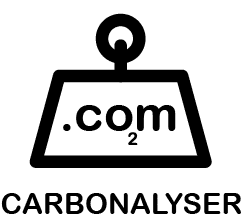
\includegraphics[width=0.3\textwidth]{imagenes/Carbonalyser_Logo.png}
\end{center}

\href{https://theshiftproject.org/en/}{https://theshiftproject.org/en/}

\href{https://addons.mozilla.org/es-ES/firefox/addon/carbonalyser/}{https://addons.mozilla.org/es-ES/firefox/addon/carbonalyser/}

\href{https://github.com/carbonalyser/Carbonalyser}{https://github.com/carbonalyser/Carbonalyser}

\textbf{Carbonalyser} es una extensión de navegador gratuita que permite visualizar el impacto ambiental del uso de Internet. Estima las emisiones de carbono derivadas de la navegación web a partir de la cantidad de datos transmitidos, utilizando el modelo \textbf{"1byte"}\footnote{Modelo de estimación del consumo energético y emisiones de CO\textsubscript{2} basado en la cantidad de datos transmitidos por Internet, propuesto por \textit{The Shift Project}.} desarrollado por \textit{The Shift Project}. A través de esta herramienta, los usuarios pueden comprender mejor el impacto de su navegación en términos de consumo energético y emisiones de CO\textsubscript{2}, ajustado a la intensidad de carbono de su región.

Está disponible para \textbf{Firefox}, y existen versiones \textit{fork} para
\textbf{Chrome} y \textbf{Edge}, lo que facilita su instalación y uso. La
extensión procesa toda la información de manera \textbf{local}, sin enviar
datos a servidores externos, lo que garantiza la privacidad del usuario. La
visualización es intuitiva, mostrando un ranking de sitios web, datos
transmitidos y comparaciones con actividades físicas cotidianas (como el uso de
un móvil o la conducción).

Carbonalyser es además código abierto bajo licencia MIT, con el código alojado
en \textbf{GitHub}\footnote{Plataforma de desarrollo colaborativo basada en Git que permite almacenar, compartir y revisar
  código fuente.}. Permite configurar la ubicación eléctrica para ajustar las
estimaciones a la \textbf{intensidad de carbono regional}\footnote{Valor medio de emisiones por kWh en una región concreta, utilizado para estimar el impacto energético del centro de datos.}, ayudando a que el análisis
sea más contextual y educativo.

\subsection*{Puntos fuertes:}

\begin{itemize}
  \item \textbf{Muy fácil de usar}: instalación rápida en Firefox (y forks disponibles para Chrome y Edge).
  \item \textbf{Procesamiento 100\% local}: no transmite datos a terceros, garantizando privacidad.
  \item \textbf{Visualización clara y educativa}: rankings, comparativas y equivalencias comprensibles.
  \item \textbf{Código abierto y gratuito}: bajo licencia MIT, con comunidad en GitHub.
  \item \textbf{Cálculo adaptado por región}: permite configurar la localización eléctrica del usuario.
  \item \textbf{Herramienta útil para educación}: ideal para concienciar sobre sostenibilidad digital.
\end{itemize}

\subsection*{Puntos débiles:}

\begin{itemize}
  \item \textbf{Limitado al tráfico web}: no mide el impacto de componentes fuera del navegador.
  \item \textbf{Basado en modelos generalistas}: utiliza estimaciones teóricas ("1byte"), no mediciones de hardware reales.
  \item \textbf{No almacena datos históricos}: se reinicia al cerrar el navegador, sin seguimiento continuo.
  \item \textbf{No integrable en otros sistemas}: no puede incorporarse a software externo o pipelines.
  \item \textbf{Desarrollo inactivo}: última versión publicada en 2020, con escasa evolución desde entonces.
  \item \textbf{Permisos elevados}: requiere acceso a pestañas y solicitudes web, lo que puede generar reticencias en entornos corporativos.
  \item \textbf{Cálculo adaptado por región limitado}: Solo permite elegir entre regiones muy amplias como Europa o Estados Unidos, lo que hace menos preciso el cálculo.
\end{itemize}

\section*{\textbf{GreenFrame}}

\begin{center}

\includegraphics[width=0.3\textwidth]{imagenes/GreenFrame_Logo.png}
\end{center}

\url{https://greenframe.io/}

\url{https://docs.greenframe.io/}

\url{https://marmelab.com/en/}

\textbf{GreenFrame} es una solución enfocada en medir el consumo energético y las emisiones de carbono generadas por aplicaciones web durante su ejecución. Permite realizar auditorías detalladas mediante una combinación de herramientas como una interfaz web, una línea de comandos (CLI) y escenarios personalizables a través de \textbf{Playwright}\footnote{Herramienta de automatización de pruebas web que permite simular acciones del usuario (clics, escritura, navegación) en navegadores reales.}, lo que permite simular interacciones reales con la aplicación.

Es especialmente útil en entornos de desarrollo, ya que permite comparar el
impacto entre versiones de una misma aplicación o entre diferentes páginas.
También se puede integrar con \textbf{GitHub} para bloquear automáticamente \textbf{pull
  requests}\footnote{Solicitud para fusionar cambios de una rama a otra en un
  repositorio Git, sujeta a revisión antes de ser aceptada.} que superen un
umbral de emisiones establecido, contribuyendo a una cultura
\textbf{DevOps}\footnote{Práctica que integra desarrollo (Dev) y operaciones
  (Ops) para agilizar la entrega y mejorar la calidad del software.} más
sostenible.

GreenFrame realiza un análisis de \textbf{pila completa}, teniendo en cuenta el
uso de CPU, red, memoria, disco y \textbf{PUE}\footnote{(Power Usage
  Effectiveness) Métrica para evaluar la eficiencia energética de un centro de
  datos.} (Power Usage Effectiveness), con distinción entre tráfico
\textbf{intranet} e \textbf{internet}. Está basado en un modelo científico
desarrollado junto al \textbf{CNRS}\footnote{Centro Nacional de Investigación
  Científica de Francia. Participa en el modelo científico detrás de GreenFrame.}
(Centro Nacional para la Investigación Científica de Francia), que ha sido
\textbf{validado académicamente}.

\textbf{Puntos fuertes:}
\begin{itemize}
  \item \textbf{Alta precisión y detalle}: mide múltiples métricas (CPU, memoria, red, disco, PUE), diferenciando tráfico local y externo.
  \item \textbf{Pensado para desarrolladores}: comparativas entre versiones y páginas específicas.
  \item \textbf{Soporta distintos niveles de análisis}: desde páginas individuales hasta aplicaciones completas (\textit{full-stack}).
  \item \textbf{Integración CI/CD}: integración con GitHub para evitar merges si se supera un umbral de emisiones.
  \item \textbf{Modelo validado científicamente}: desarrollado con el CNRS, transparente en metodología general.
\end{itemize}

\textbf{Puntos débiles:}
\begin{itemize}
  \item \textbf{Modelo parcialmente cerrado}: la conversión a energía y CO$_2$ no es completamente transparente (algunos elementos son secretos comerciales).
  \item \textbf{Limitaciones en versión gratuita}: no incluye almacenamiento histórico ni visualización temporal; requiere conocimientos técnicos para usar la CLI.
  \item \textbf{No modela interacciones largas}: se centra en visitas individuales, sin simular sesiones prolongadas.
  \item \textbf{Web UI completa solo en plan Enterprise}: requiere suscripción de pago
        (12€/usuario/mes).
  \item \textbf{Curva de aprendizaje}: uso de CLI y Playwright implica mayor complejidad técnica.
\end{itemize}

\section*{\textbf{Website Carbon Calculator}}

\begin{center}
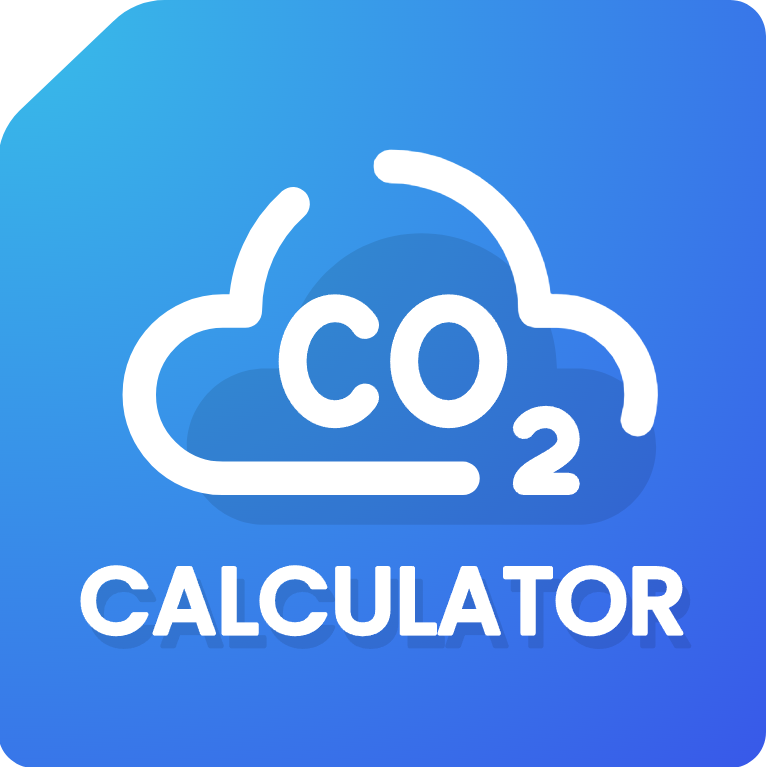
\includegraphics[width=0.3\textwidth]{imagenes/Website_Logo.png}
\end{center}

\url{https://www.websitecarbon.com/}

\url{https://www.websitecarbon.com/how-does-it-work/}

\textbf{Website Carbon Calculator} es una herramienta online gratuita que estima la huella de carbono de un sitio web analizando factores como el peso de la página, los recursos cargados, el tipo de contenido y la localización del servidor. Proporciona una puntuación energética (de la \textbf{A a la G}), una estimación de emisiones por visita y recomendaciones prácticas para mejorar la eficiencia.

Está pensada para facilitar una primera \textbf{auditoría}\footnote{Evaluación
  sistemática de una página web para determinar su eficiencia energética y huella
  digital.} accesible y sin conocimientos técnicos previos, siendo ideal para
usuarios no técnicos, diseñadores web y campañas de sensibilización. También
ofrece una \textbf{API REST}\footnote{Interfaz de programación que permite
  acceder a los servicios del sitio mediante solicitudes HTTP automatizadas.}
para integraciones automatizadas.

\textbf{Puntos fuertes:}
\begin{itemize}
  \item \textbf{Extremadamente accesible}: no requiere conocimientos técnicos.
  \item \textbf{Rápido y visual}: análisis en pocos segundos con resultados claros.
  \item \textbf{Comparación global}: útil para campañas de concienciación y benchmarking.
  \item \textbf{Gratuito y abierto}: interfaz sin coste y documentación disponible.
  \item \textbf{API disponible}: permite automatizar análisis desde scripts o plataformas externas.
\end{itemize}

\textbf{Puntos débiles:}
\begin{itemize}
  \item \textbf{Modelo simplificado}: no mide interacciones complejas ni escenarios completos.
  \item \textbf{Menor precisión técnica}: basado en estimaciones generales, no analiza procesos del lado servidor.
  \item \textbf{No incluye comportamiento dinámico}: ignora scripts posteriores a la carga inicial.
  \item \textbf{No distingue tráfico local/internacional}: aplica valores promedio que pueden no reflejar la realidad específica.
  \item \textbf{Sin personalización ni históricos}: cada análisis es aislado, sin seguimiento temporal.
\end{itemize}

\section*{\textbf{Ecograder}}

\begin{center}

\includegraphics[width=0.3\textwidth]{imagenes/Ecograder_Logo.png}
\end{center}

\url{https://ecograder.com/}

\textbf{Ecograder} es una herramienta gratuita que analiza la sostenibilidad de sitios web desde una perspectiva técnica y ambiental. Proporciona una puntuación de 1 a 100 basada en criterios como eficiencia del frontend, peso de la página, experiencia de usuario (UX) y uso de hosting sostenible. Utiliza el script \textbf{CO2.js}\footnote{Biblioteca de código abierto que estima las emisiones de carbono de una página web basándose en cuatro áreas: dispositivo, red, servidor y hardware.} para calcular las emisiones estimadas de carbono.

Es ideal para consultoras, desarrolladores web y diseñadores que buscan evaluar
y mejorar la eficiencia ambiental de sus sitios de forma rápida, sin necesidad
de configuración ni conocimientos avanzados.

\textbf{Puntos fuertes:}
\begin{itemize}
  \item \textbf{Interfaz visual e intuitiva}: muestra resultados desglosados por categoría (peso, UX, hosting), con gráficas y explicaciones claras.
  \item \textbf{Puntuación global (1–100)}: facilita la interpretación rápida del rendimiento ecológico de un sitio web.
  \item \textbf{Recomendaciones técnicas útiles}: incluye sugerencias concretas como minificar recursos, reducir llamadas HTTP, o cambiar a un proveedor de hosting verde.
  \item \textbf{Basado en CO2.js}: ofrece transparencia y confianza al usar una metodología reconocida y de código abierto para estimar emisiones.
  \item \textbf{Acceso instantáneo}: sólo requiere introducir una URL para obtener el análisis, sin necesidad de registro ni instalación.
  \item \textbf{Evaluación multidimensional}\footnote{Análisis que contempla varios factores técnicos y ambientales, como eficiencia del código, UX, tamaño de archivos y uso de energía sostenible.}: considera tanto eficiencia técnica como prácticas sostenibles (energía renovable, peso de recursos, etc.).
\end{itemize}

\textbf{Puntos débiles:}
\begin{itemize}
  \item \textbf{Limitado al frontend}: no evalúa consumo energético de servidores, APIs, bases de datos u otros elementos backend, solo hace una estimación del consumo energético basada en el tráfico de red y la intensidad de carbono regional.
  \item \textbf{Resultados poco estables}: las puntuaciones pueden variar entre análisis consecutivos debido a cambios dinámicos en el sitio o actualizaciones de la propia herramienta.
  \item \textbf{Sin simulaciones de usuario}: no permite crear escenarios personalizados ni medir la huella en flujos de interacción reales.
  \item \textbf{No guarda históricos}: no permite comparar resultados a lo largo del tiempo ni registrar progresos entre versiones.
  \item \textbf{Un solo análisis por vez}: no se pueden evaluar varias páginas simultáneamente desde la interfaz actual ya que aún no cuentan con una API.
\end{itemize}

\section*{\textbf{CodeCarbon}}

\begin{center}

\includegraphics[width=0.3\textwidth]{imagenes/CodeCarbon_Logo.jpg}
\end{center}

\url{https://codecarbon.io/}

\url{https://mlco2.github.io/codecarbon/}

\textbf{CodeCarbon} es una biblioteca ligera de Python diseñada para estimar las emisiones de CO$_2$ asociadas a la ejecución de scripts y procesos computacionales. Calcula el consumo energético de CPU, GPU y RAM, y convierte estos datos en emisiones aproximadas según la \textbf{intensidad de carbono regional} de la región geográfica donde se ejecuta el código. Se integra fácilmente mediante \textbf{decoradores}\footnote{Función en Python que modifica el comportamiento de otra función o método.} o \textbf{gestores de contexto}\footnote{Estructura que gestiona recursos con `with` en Python.}.

Es una solución ideal para proyectos de ciencia de datos, *machine learning* o
cualquier \textbf{pipeline}\footnote{Secuencia automatizada de procesos o
  tareas en datos o código.} Python que quiera monitorizar su huella de carbono.

\textbf{Puntos fuertes:}
\begin{itemize}
  \item \textbf{Integración sencilla en Python}: basta con añadir un \textbf{decorador\textsuperscript{2}} o usar un bloque \texttt{with}, sin alterar significativamente el código.
  \item \textbf{Contextualización clara de resultados}: incluye equivalencias (km en coche, horas de televisión) para entender el impacto.
  \item \textbf{Modos online y offline}: online obtiene intensidad de carbono actualizada vía APIs como \textbf{ElectricityMap}\footnote{Servicio que ofrece datos sobre intensidad de carbono del consumo eléctrico en tiempo real.}; offline permite especificar región manualmente (códigos ISO).
  \item \textbf{Ligero y eficiente}: pensado para no ralentizar significativamente los procesos.
  \item \textit{Útil en notebooks, scripts y pipelines de \textbf{CI/CD}}: encaja en \textbf{Jupyter Notebooks}\footnote{Entorno interactivo para escribir y ejecutar código en Python.}, *scripts* y cualquier pipeline mediante \textbf{CLI} o decoradores.
  \item \textbf{Comunidad activa y bien documentado}: disponible en \textbf{PyPI\textsuperscript{12}}, con ejemplos y documentación clara.
\end{itemize}

\textbf{Puntos débiles:}
\begin{itemize}
  \item \textbf{Dependencia de datos externos}: precisión limitada si la API de intensidad de carbono no está actualizada.
  \item \textbf{Sin simulaciones de usuario}: no mide flujos de interacción reales, solo bloques de código.
  \item \textbf{Requiere configuración previa}: es necesario generar y gestionar el archivo de configuración.
  \item \textbf{Almacenamiento local}: offline solo guarda en `.csv`, sin historiales automáticos.
  \item \textbf{Sin API propia para análisis masivo}: no permite evaluar múltiples proyectos simultáneamente desde la web.
\end{itemize}

\begin{section}{\textbf{Conclusiones de la comparativa de herramientas}}
 % Cambiar a orientación paisaje para la tabla
 \begin{landscape}

   % Colores
   \definecolor{header1}{RGB}{33, 150, 243}   % Azul
   \definecolor{header2}{RGB}{76, 175, 80}    % Verde
   \definecolor{header3}{RGB}{244, 67, 54}    % Rojo
   \definecolor{rowlight}{RGB}{245,245,245}

   % Iconos ✔ y ✘ dentro de círculos con TikZ (más grandes)
   \newcommand{\yes}{\tikz\draw[fill=green!70!black,draw=none] (0,0) circle (0.2) node[white,scale=1.2]{\checkmark};}
   \newcommand{\no}{\tikz\draw[fill=red!80!black,draw=none] (0,0) circle (0.2) node[white,scale=1.2]{\textsf{x}};}
   \newcommand{\casi}{\tikz\draw[fill=orange!80!black,draw=none] (0,0) circle (0.2) node[white,scale=1.2]{\text{*}};}

   % Filas alternas
   \rowcolors{2}{rowlight}{white}

   % Espaciado más compacto
   \renewcommand{\arraystretch}{1.2}

   % Primera tabla: Criterios 1, 2 y 3
   \resizebox{\linewidth}{!}{%
     \begin{tabular}{|l|c|c|c|c|c|c|c|c|c|}
       % Fila adicional con nombres destacados
                                                                      &
       \multicolumn{1}{c|}{\color{black}\textbf{\large AWS}}          &
       \multicolumn{1}{c|}{\color{black}\textbf{\large Impact}}       &
       \multicolumn{1}{c|}{\color{black}\textbf{\large Carbon}}       &
       \multicolumn{1}{c|}{\color{black}\textbf{\large Cloud}}        &
       \multicolumn{1}{c|}{\color{black}\textbf{\large Carbonalyser}} &
       \multicolumn{1}{c|}{\color{black}\textbf{\large GreenFrame}}   &
       \multicolumn{1}{c|}{\color{black}\textbf{\large Website}}      &
       \multicolumn{1}{c|}{\color{black}\textbf{\large Ecograder}}    &
       \multicolumn{1}{c|}{\color{black}\textbf{\large CodeCarbon}}                                                           \\

       \toprule
       \textbf{1. Precisión y Fiabilidad del Cálculo}                 & \multicolumn{9}{c|}{}                                 \\
       \midrule
       Adopción del estándar SCI                                      & \no                   & \yes & \no & \no & \no & \no & \no & \no & \no \\
       Modelos de estimación documentados                             & \casi                 & \yes & \casi & \yes & \yes & \casi & \yes & \yes & \yes \\
       Contextualización regional                                     & \yes                  & \yes & \yes & \yes & \yes & \no & \casi & \casi & \yes \\
       Transparencia metodológica                                     & \no                  & \yes & \casi & \yes & \yes & \casi & \yes & \yes & \yes \\
       Validación de resultados                                       & \no                  & \casi & \casi & \casi & \no & \casi & \casi & \casi & \casi \\
       \midrule
       \textbf{2. Cobertura y Alcance}                                & \multicolumn{9}{c|}{}                                 \\
       \midrule
       Entornos locales                                               & \no                   & \yes & \casi & \casi & \no & \casi & \no & \no & \yes \\
       Entornos cloud                                                 & \casi                  & \yes & \yes & \yes& \no & \casi & \no & \no & \yes \\
       Scope 1, 2 y 3                                                 & \casi                  & \casi & \no & \yes & \no & \no & \casi & \no & \casi \\
       Granularidad por componente                                    & \yes                  & \yes & \no & \yes & \casi & \yes & \casi & \casi & \yes \\
       Proyecciones futuras                                           & \yes                  & \no & \casi & \no & \no & \no & \no & \no & \no \\
       Carbono incorporado hardware                                   & \no                  & \no & \no & \yes & \no & \no & \casi & \no & \no \\
       \midrule
       \textbf{3. Facilidad de Integración y Uso}                     & \multicolumn{9}{c|}{}                                 \\
       \midrule
       Interfaz web                                                   & \yes                  & \no & \no & \yes & \yes & \yes & \yes & \yes & \casi \\
       Interfaz CLI                                                   & \no                   & \yes & \yes & \yes & \no & \yes & \no & \no & \yes \\
       API REST                                                       & \casi                  & \casi & \yes & \yes & \no & \casi & \casi & \no & \no \\
       SDK disponible                                                 & \no                   & \yes & \yes & \casi & \no & \no & \no & \no & \yes \\
       Integración CI/CD                                              & \no                  & \yes & \yes & \casi& \no & \yes & \no & \no & \casi \\
       Visualización interactiva                                      & \yes                  & \no & \no & \yes & \yes & \yes & \yes & \yes & \yes \\
       \bottomrule
     \end{tabular}
   }%

   \vspace{2cm}

   % Segunda tabla: Criterios 4 y 5
   \resizebox{\linewidth}{!}{%
     \begin{tabular}{|l|c|c|c|c|c|c|c|c|c|}
       % Fila adicional con nombres destacados
                                                                      &
       \multicolumn{1}{c|}{\color{black}\textbf{\large AWS}}          &
       \multicolumn{1}{c|}{\color{black}\textbf{\large Impact}}       &
       \multicolumn{1}{c|}{\color{black}\textbf{\large Carbon}}       &
       \multicolumn{1}{c|}{\color{black}\textbf{\large Cloud}}        &
       \multicolumn{1}{c|}{\color{black}\textbf{\large Carbonalyser}} &
       \multicolumn{1}{c|}{\color{black}\textbf{\large GreenFrame}}   &
       \multicolumn{1}{c|}{\color{black}\textbf{\large Website}}      &
       \multicolumn{1}{c|}{\color{black}\textbf{\large Ecograder}}    &
       \multicolumn{1}{c|}{\color{black}\textbf{\large CodeCarbon}}                                                           \\

       \toprule
       \textbf{4. Accesibilidad y Usabilidad}                         & \multicolumn{9}{c|}{}                                 \\
       \midrule
       Curva de aprendizaje baja                                      & \casi                  & \no & \casi & \casi & \yes & \yes & \yes & \yes & \yes \\ 
       Configuración guiada                                           & \no                  & \casi & \no & \casi & \yes & \yes & \yes & \yes & \yes \\
       Adaptación a perfiles                                          & \no                  & \no & \no & \yes & \no & \casi & \no & \no & \casi \\
       Equivalencias comprensibles                                    & \no                   & \no & \no & \no & \yes & \no & \no & \yes & \yes \\
       Sistema de puntuación                                          & \no                   & \yes & \no & \no & \no & \no & \yes & \yes & \no \\
       Recomendaciones personalizadas                                 & \casi                  & \no & \casi & \no & \casi & \no & \no & \yes & \casi \\
       \midrule
       \textbf{5. Capacidad de Exportación y Reporte}                 & \multicolumn{9}{c|}{}                                 \\
       \midrule
       Exportación CSV/JSON                                           & \yes                  & \yes & \casi & \yes & \no & \no & \no & \no & \yes \\
       Generación de informes                                         & \yes                  & \casi & \no & \casi & \no & \casi & \no & \casi & \yes \\
       Historial y seguimiento                                        & \yes                  & \casi & \casi & \yes & \no & \yes & \no & \no & \yes \\
       Comparativas y benchmarks                                      & \casi                  & \casi & \casi & \casi & \casi & \yes & \casi & \no & \casi \\
       \bottomrule
     \end{tabular}
   }%

 \end{landscape}

\end{section}

\chapter{Propuesta de implementación de EcoCode}

\section{Propuesta de valor}

\section{Diseño de la interfaz de usuario}

\chapter{Diseño Técnico}

\section{Historia de desarrollo}

\section{Diseño de pruebas}

\chapter{Documentación}

\section{Publicacion}

\chapter{Conclusiones y trabajos futuros}

% Bibliografía
\chapter*{Bibliografía}
\addcontentsline{toc}{chapter}{Bibliografía}
\begin{thebibliography}{99}
  \bibitem{ref1}\hypertarget{bib:1}{}\href{https://www.acciona.com/es/cambio-climatico}{ACCIONA - Cambio Climático.}

  \bibitem{ref2}\hypertarget{bib:2}{}\href{https://www.sostenibilidad.com/cambio-climatico/impactos-cambio-climatico/}{Sostenibilidad - Impactos del Cambio Climático. }

  \bibitem{ref3}\hypertarget{bib:3}{}\href{https://www.who.int/es/news-room/fact-sheets/detail/climate-change-and-health}{Organización Mundial de la Salud - Cambio climático y salud. }

  \bibitem{ref4}\hypertarget{bib:4}{}\href{https://unfccc.int/es/acerca-de-las-ndc/el-acuerdo-de-paris}{UNFCCC - El Acuerdo de París. }

  \bibitem{ref5}\hypertarget{bib:5}{}\href{https://sci.greensoftware.foundation/}{Green Software Foundation - Software Carbon Intensity (SCI) Specification}

  \bibitem{ref6}\hypertarget{bib:6}{}\href{https://www.v2.ai/insights/how-green-is-your-software-unravelling-the-software-carbon-intensity}{Michael Zajer - How Green is your Software? Unravelling the SCI}

  \bibitem{ref7}\hypertarget{bib:7}{}\href{https://greenlab.di.uminho.pt/wp-content/uploads/2017/10/sleFinal.pdf}{Pereira et al. - Energy efficiency across programming languages}

  \bibitem{ref8}\hypertarget{bib:8}{}\href{https://app.electricitymaps.com/map}{Electricity Maps - Live CO2 emissions of electricity consumption}

  \bibitem{ref9}\hypertarget{bib:9}{}\href{https://www.techcarbonstandard.org/technology-categories/lifecycle/example/server}{Data Centre and Server Hardware Example Emissions}
\end{thebibliography}

\appendix
\chapter{Anexos}
\section{Configuracion y uso de herramientas analizadas}
\subsection{AWS customer carbon footprint tool}
\begin{enumerate}
  \item Iniciar sesión con tu cuenta en la consola de AWS y abrir Billing and Cost
        Management.
  \item En el menú lateral, seleccionar \textbf{Customer Carbon Footprint Tool}.
  \item Elegir el \textbf{mes de inicio} y el \textbf{mes de fin}.
\end{enumerate}
Esto mostrará una vista con la \textbf{información} de nuestras emisiones, permitiéndonos revisar el periodo de tiempo que deseemos.
\begin{center}
  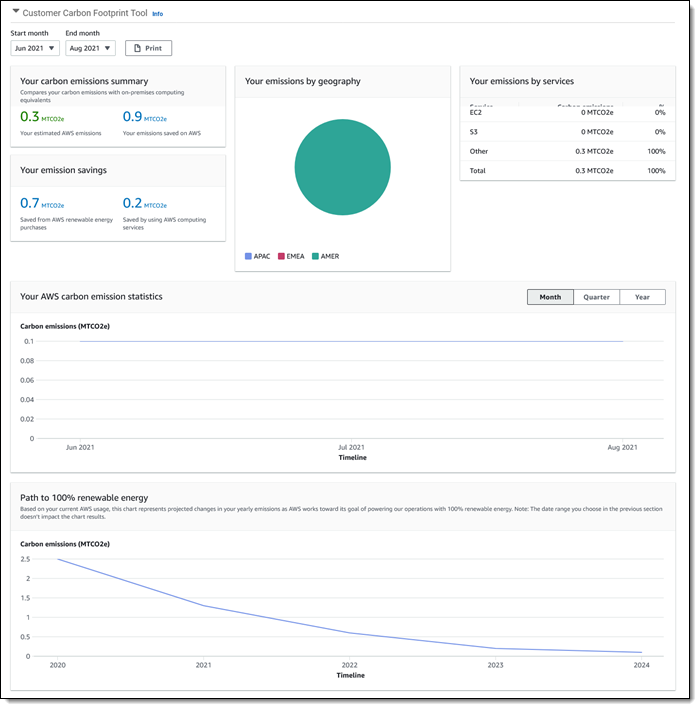
\includegraphics[width=0.8\textwidth]{imagenes/AWS_1.png}
  \captionof{figure}{Vista de la herramienta AWS Customer Carbon Footprint Tool.}
\end{center}

\subsection{Impact Framework}
Se puede probar instalándolo en nuestro equipo mediante el \textbf{gestor de
  paquetes} npm\footnote{Herramienta que instala y gestiona librerías o
  herramientas, como npm para proyectos JavaScript.}:

\begin{tcolorbox}[colback=codebackground, colframe=codeborder, boxrule=0.8pt, arc=0mm, boxsep=5pt, left=5pt, right=5pt, top=5pt, bottom=5pt]
  \begin{lstlisting}[language=bash]
  npm install -g @grnsft/if
  \end{lstlisting}
\end{tcolorbox}

Creamos un fichero \textbf{IMP}\footnote{Archivo de configuración de Impact
  Framework en formato YAML; define qué métricas y plugins usar.} con la
extensión \textbf{.yml}\footnote{Archivo de configuración de Impact Framework
  en formato YAML; define qué métricas y plugins usar.}, el cual contendrá las
configuraciones y los datos necesarios para medir el impacto energético y
ambiental de nuestra aplicación:

\begin{center}
  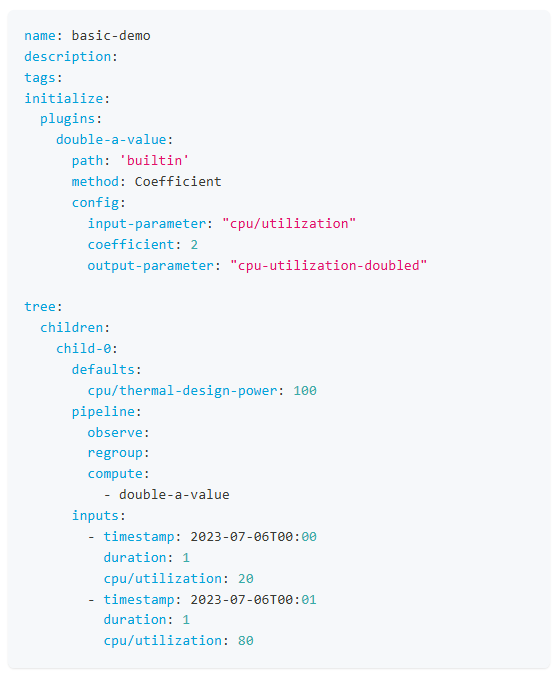
\includegraphics[width=0.8\textwidth]{imagenes/IF_1.png}
  \captionof{figure}{Archivo IMP de ejemplo}
\end{center}

Tras esto, lo podemos ejecutar con:

\begin{tcolorbox}[colback=codebackground, colframe=codeborder, boxrule=0.8pt, arc=0mm, boxsep=5pt, left=5pt, right=5pt, top=5pt, bottom=5pt]
  \begin{lstlisting}[language=bash]
  if-run --IMP <path-to-your-IMP>
  \end{lstlisting}
\end{tcolorbox}

\subsection{Carbon Aware SDK}
Para usarlo por \textbf{CLI} necesitamos
tener \textbf{.NET Core}\footnote{Plataforma de ejecución multiplataforma de
  Microsoft para construir y ejecutar aplicaciones.} (o usar
\textbf{Docker}\footnote{Motor de contenedores que empaqueta aplicaciones con
  sus dependencias para ejecución aislada.} con VSCode y Remote Containers).
Clonamos el repositorio con:

\begin{tcolorbox}[colback=codebackground, colframe=codeborder, boxrule=0.8pt, arc=0mm, boxsep=5pt, left=5pt, right=5pt, top=5pt, bottom=5pt]
  \begin{lstlisting}[language=bash]
git clone https://github.com/Green-Software-Foundation/carbon-aware-sdk.git
\end{lstlisting}
\end{tcolorbox}

y accedemos a la carpeta:

\begin{tcolorbox}[colback=codebackground, colframe=codeborder, boxrule=0.8pt, arc=0mm, boxsep=5pt, left=5pt, right=5pt, top=5pt, bottom=5pt]
  \begin{lstlisting}[language=bash]
cd carbon-aware-sdk/src/CarbonAware.CLI/src
\end{lstlisting}
\end{tcolorbox}

Podemos usar datos simulados por defecto o configurar variables de entorno si
tenemos cuenta en \textbf{WattTime} o
\textbf{Electricity Maps}. Ejecutamos
comandos con:

\begin{tcolorbox}[colback=codebackground, colframe=codeborder, boxrule=0.8pt, arc=0mm, boxsep=5pt, left=5pt, right=5pt, top=5pt, bottom=5pt]
  \begin{lstlisting}[language=bash]
dotnet run
\end{lstlisting}
\end{tcolorbox}

Por ejemplo, para obtener emisiones de dos regiones en un período de tiempo:

\begin{tcolorbox}[colback=codebackground, colframe=codeborder, boxrule=0.8pt, arc=0mm, boxsep=5pt, left=5pt, right=5pt, top=5pt, bottom=5pt]
  \begin{lstlisting}[language=bash]
dotnet run emissions -l eastus,uksouth -s 2022-08-23T11:15 -e 2022-08-23T11:20
\end{lstlisting}
\end{tcolorbox}

\begin{center}
  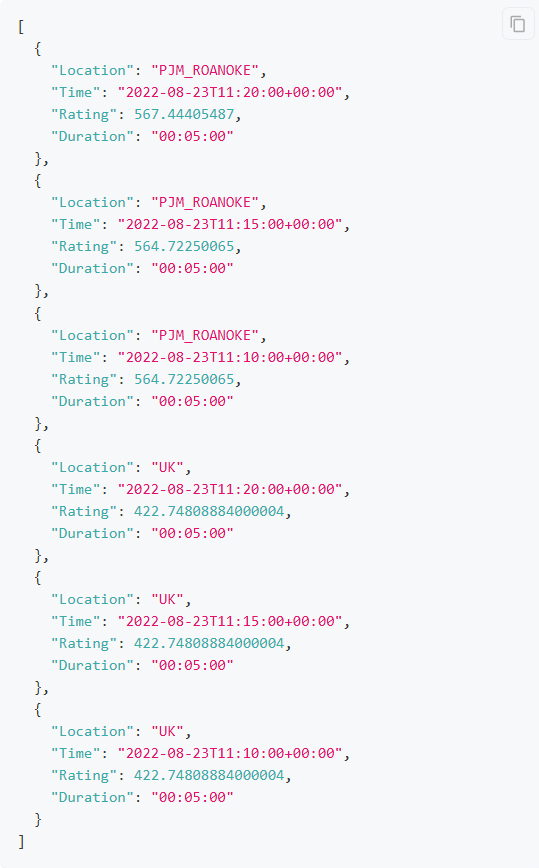
\includegraphics[width=0.8\textwidth]{imagenes/CASDK_1.png}
  \captionof{figure}{Salida del comando de emisiones para dos regiones.}
\end{center}

Y para obtener el mejor momento y la región con menos emisiones en una ventana
temporal específica:

\begin{tcolorbox}[colback=codebackground, colframe=codeborder, boxrule=0.8pt, arc=0mm, boxsep=5pt, left=5pt, right=5pt, top=5pt, bottom=5pt]
  \begin{lstlisting}[language=bash]
dotnet run emissions -l eastus,uksouth -s 2022-08-23T00:00 -e 2022-08-23T23:59 --best
\end{lstlisting}
\end{tcolorbox}

\begin{center}
  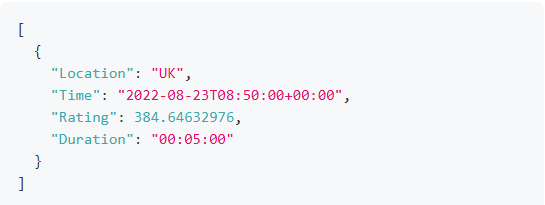
\includegraphics[width=0.8\textwidth]{imagenes/CASDK_2.png}
  \captionof{figure}{Salida del comando para encontrar el mejor momento y región para minimizar emisiones.}
\end{center}

Si preferimos la \textbf{API web} en
lugar de la \textbf{CLI}, podemos ejecutarla y
acceder a \href{http://localhost:5073}{http://localhost:5073/} y hacer llamadas
desde la consola:

\begin{tcolorbox}[colback=codebackground, colframe=codeborder, boxrule=0.8pt, arc=0mm, boxsep=5pt, left=5pt, right=5pt, top=5pt, bottom=5pt]
  \begin{lstlisting}[language=bash]
curl http://localhost:5073/locations
\end{lstlisting}
\end{tcolorbox}

Esto devolverá un \textbf{JSON}\footnote{Formato de intercambio de datos basado
  en texto, común en respuestas de APIs.} con todas las ubicaciones disponibles.
También es posible generar clientes en más de 50 lenguajes distintos usando
\textbf{OpenAPI Generator}\footnote{Herramienta que genera clientes y
  servidores en varios lenguajes a partir de especificaciones OpenAPI.}, lo que
facilita la integración en cualquier \textbf{stack}\footnote{Conjunto de
  tecnologías (lenguajes, frameworks, bases de datos) utilizadas conjuntamente en
  un proyecto.}.

\subsection{Cloud Carbon Footprint}
Para comenzar con Cloud Carbon Footprint, la forma más recomendada es crear una
aplicación independiente usando la línea de comandos. Esto se hace con el
paquete ejecutando el comando del gestor de paquetes npx:

\begin{tcolorbox}[colback=codebackground, colframe=codeborder, boxrule=0.8pt, arc=0mm, boxsep=5pt, left=5pt, right=5pt, top=5pt, bottom=5pt]
  \begin{lstlisting}[language=bash]
  npx @cloud-carbon-footprint/create-app
  \end{lstlisting}
\end{tcolorbox}

lo que te permite configurar rápidamente una instancia funcional de la
aplicación con mínima personalización.

Terminamos de configurarlo con nuestras cuentas de los distintos servicios que
queremos analizar con:

\begin{tcolorbox}[colback=codebackground, colframe=codeborder, boxrule=0.8pt, arc=0mm, boxsep=5pt, left=5pt, right=5pt, top=5pt, bottom=5pt]
  \begin{lstlisting}[language=bash]
  cd my-ccf-app
  yarn guided-install
  \end{lstlisting}
\end{tcolorbox}

Inicializamos la aplicación que hemos creado con:

\begin{tcolorbox}[colback=codebackground, colframe=codeborder, boxrule=0.8pt, arc=0mm, boxsep=5pt, left=5pt, right=5pt, top=5pt, bottom=5pt]
  \begin{lstlisting}[language=bash]
  yarn start
  \end{lstlisting}
\end{tcolorbox}

Lo cual nos sirve el frontend en
\href{http://localhost:3000}{http://localhost:3000}, en el cual se nos muestra
toda la información y podemos decidir los filtros y opciones que queramos para
una mejor visualización:

\begin{center}
  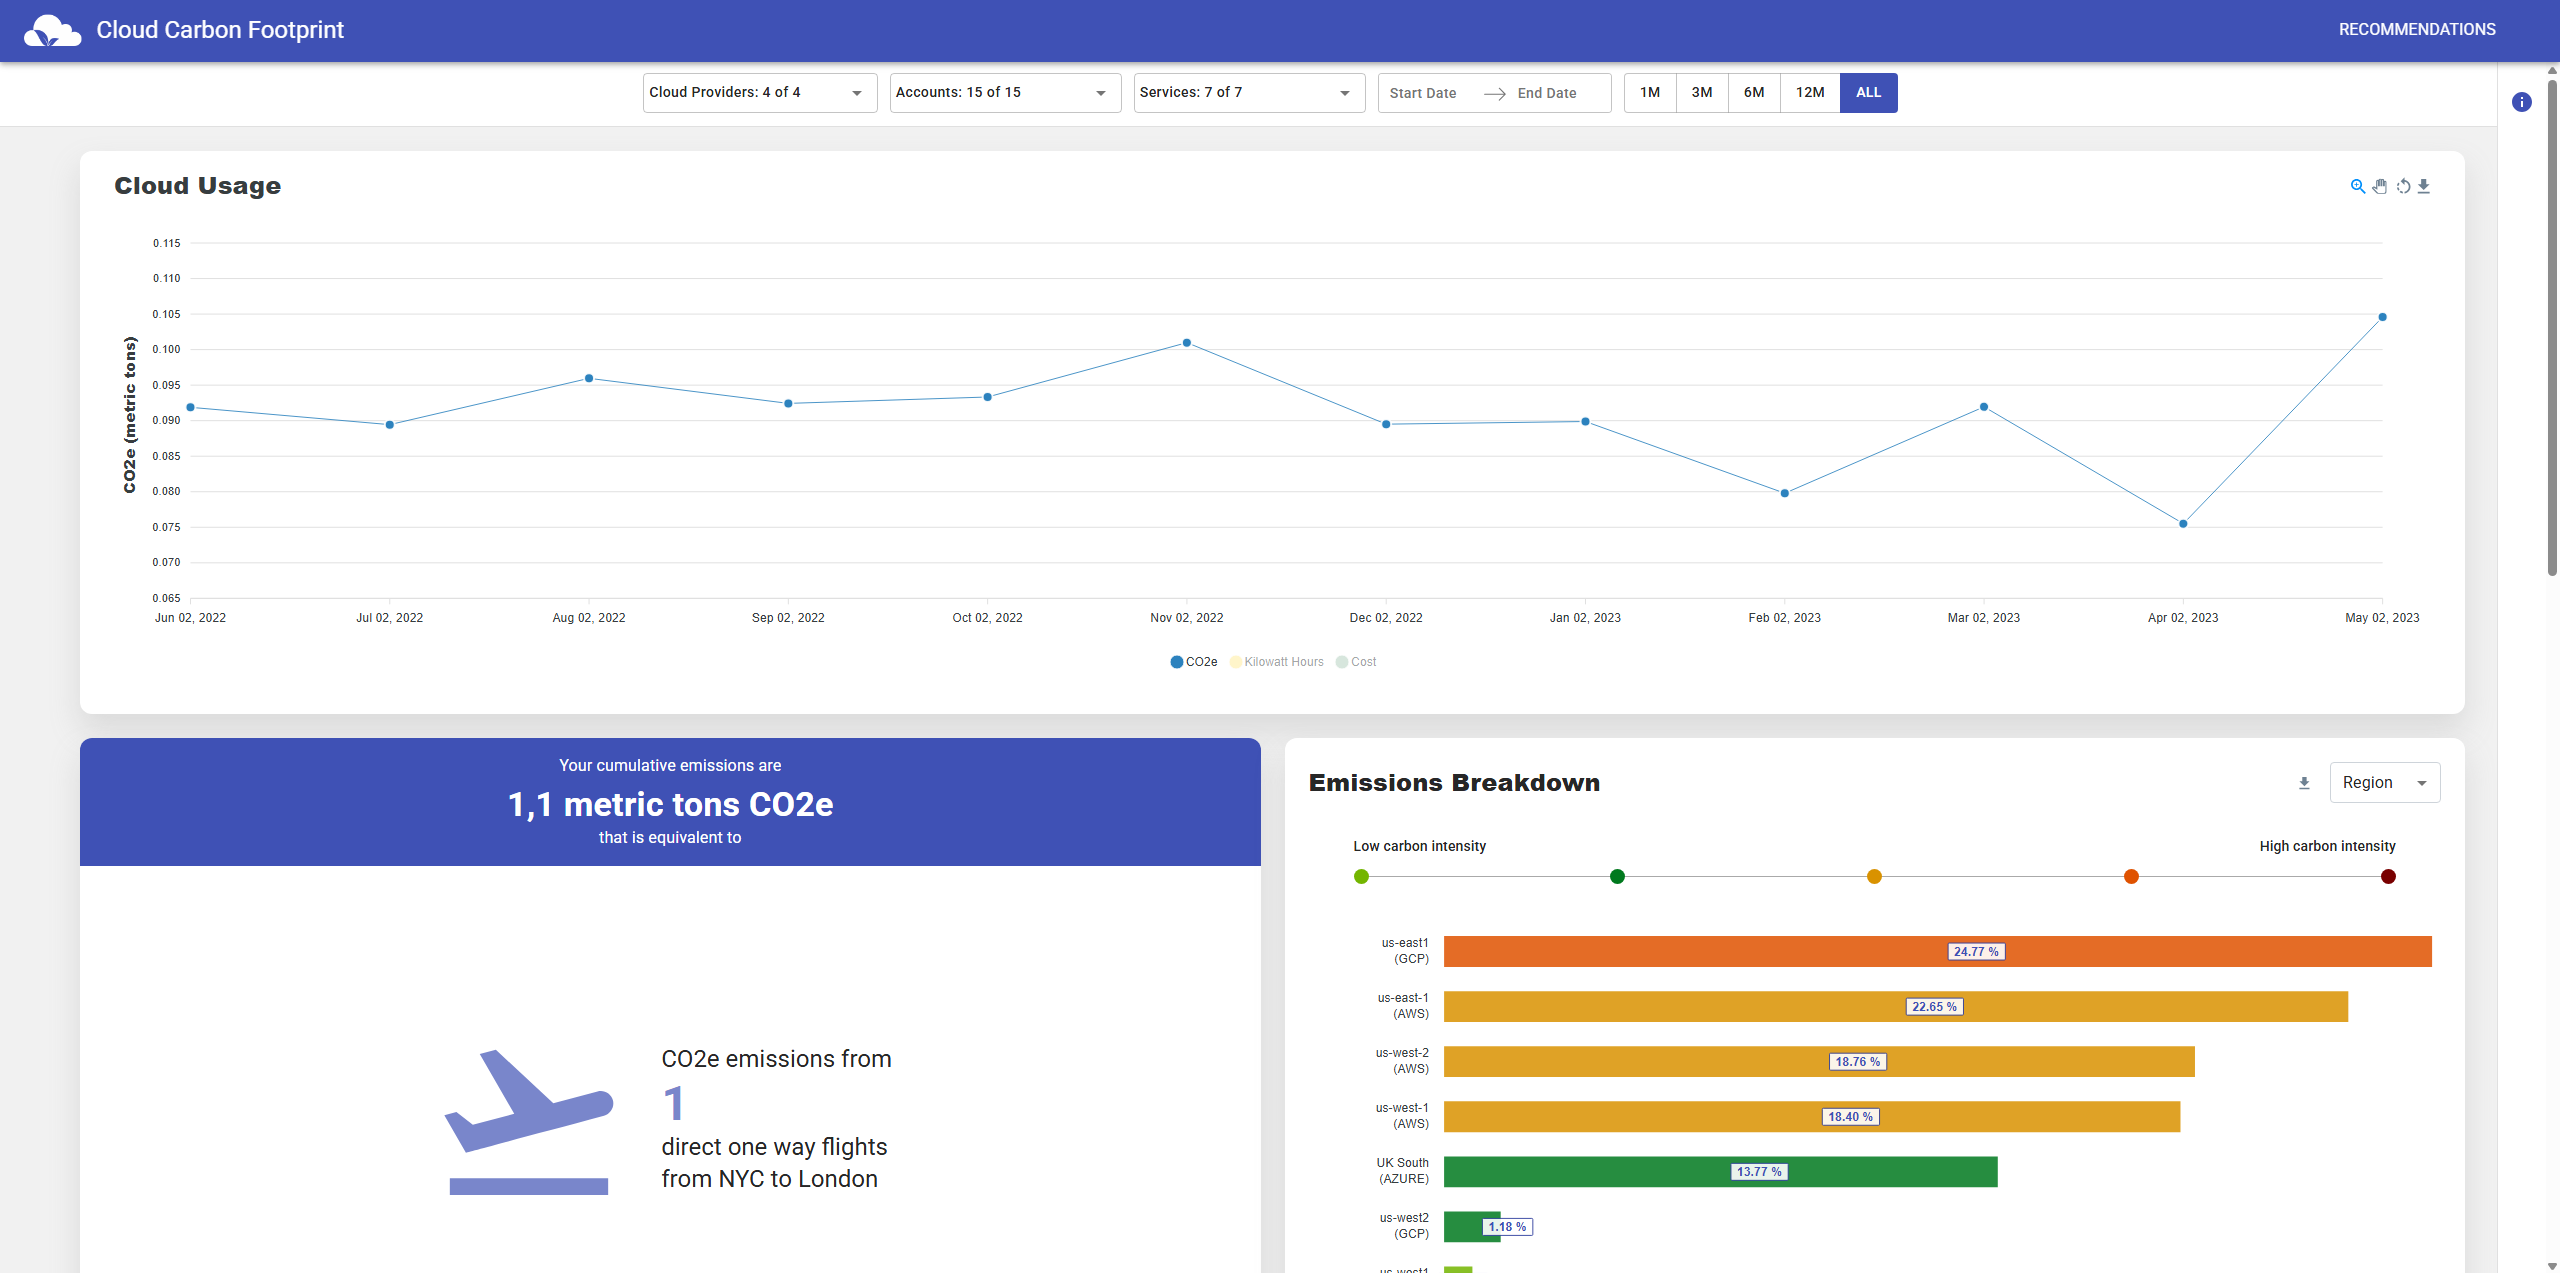
\includegraphics[width=0.8\textwidth]{imagenes/CCF_1.png}
  \captionof{figure}{Panel principal de Cloud Carbon Footprint}
\end{center}

\begin{center}
  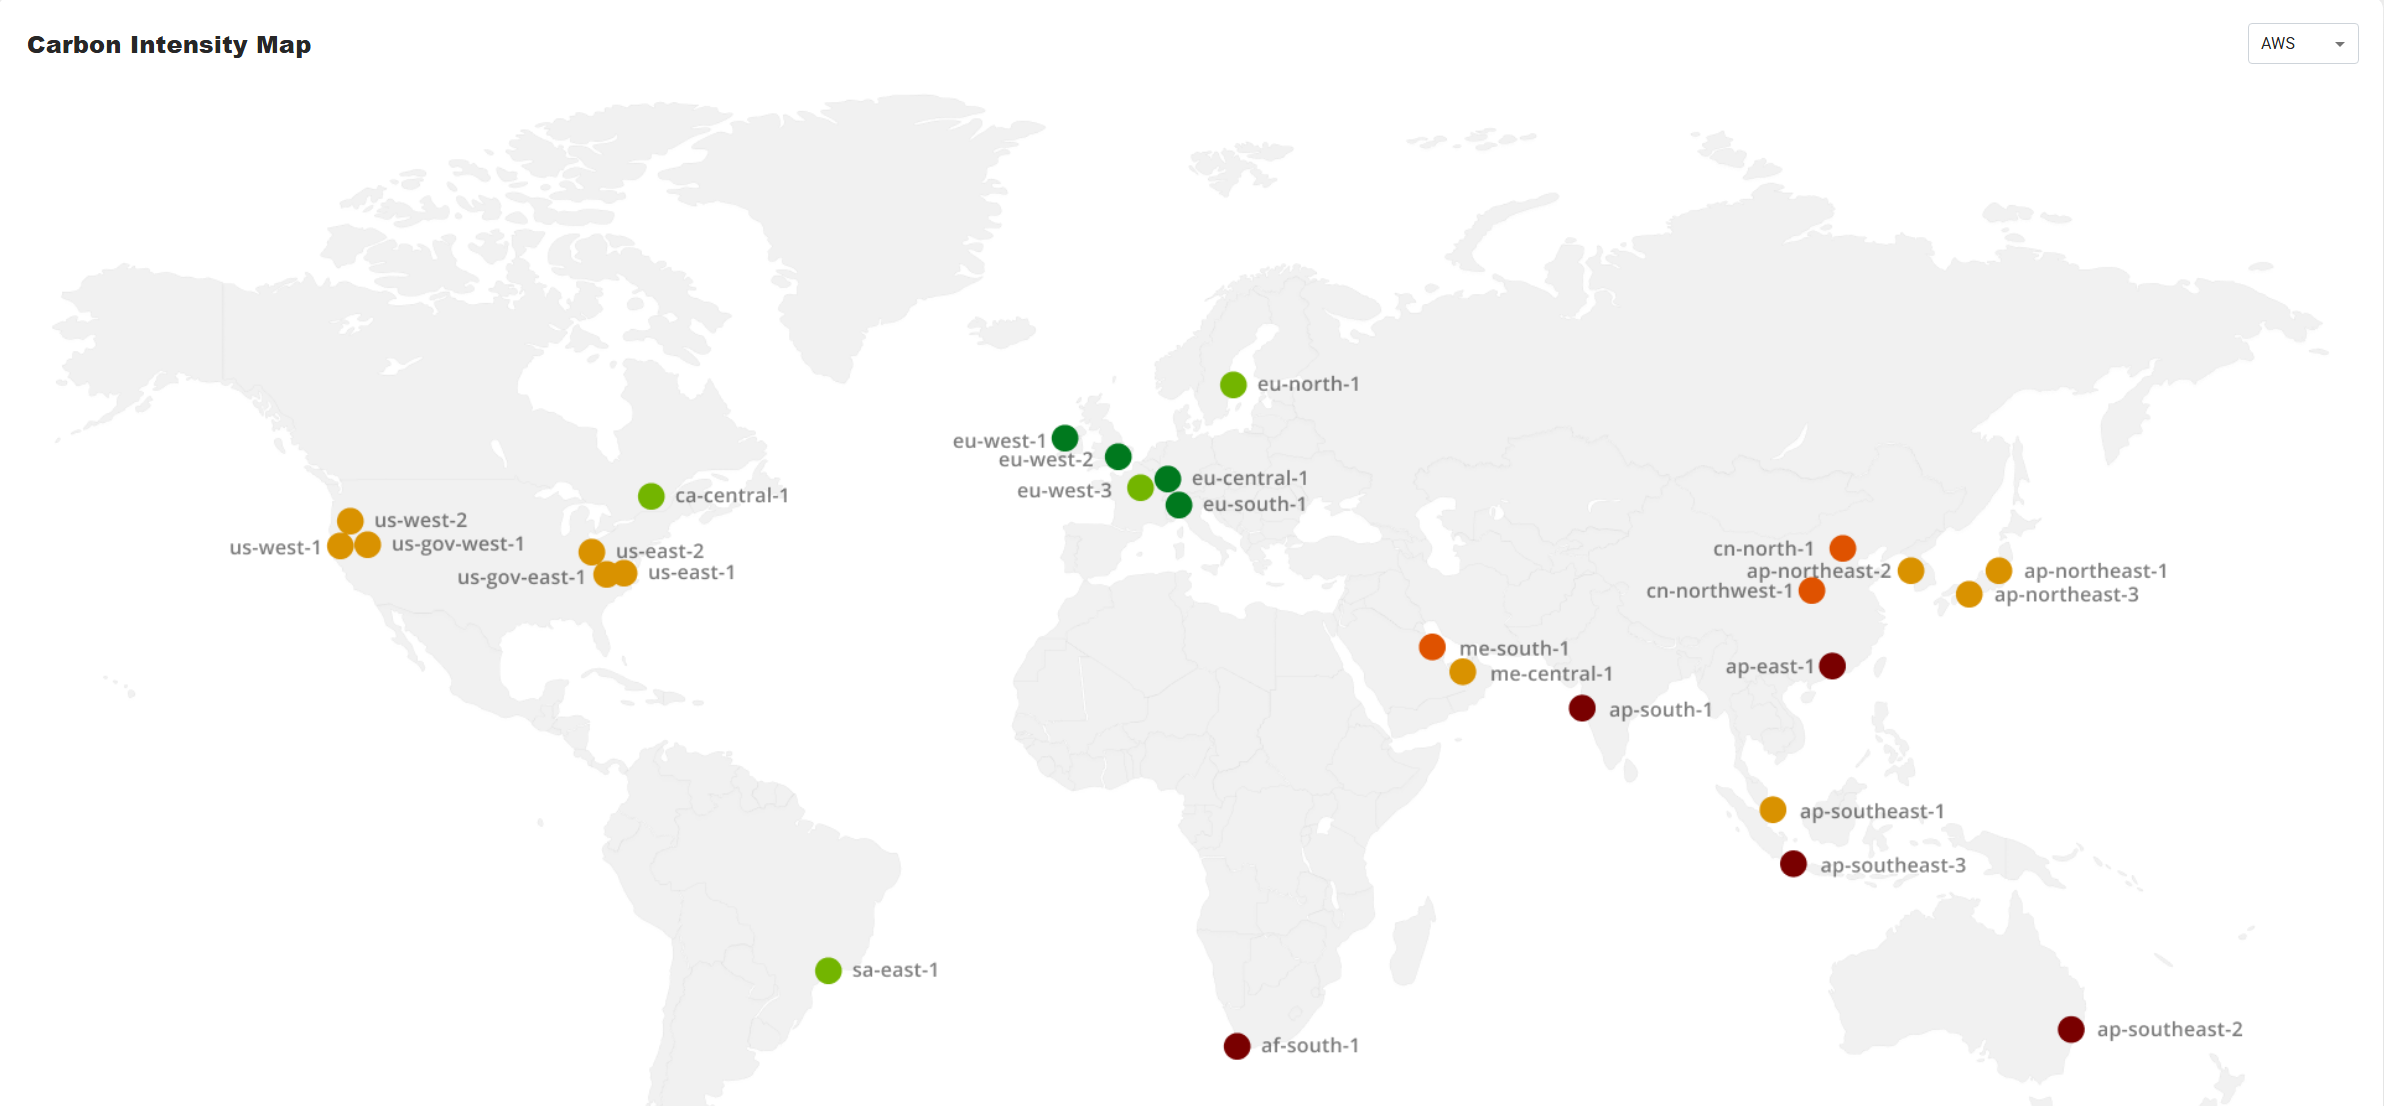
\includegraphics[width=0.8\textwidth]{imagenes/CCF_2.png}
  \captionof{figure}{Visualización de métricas en Cloud Carbon Footprint}
\end{center}

También puedes clonar el repositorio y configurar la aplicación localmente para
realizar los cambios que necesites. Otra opción es ejecutar la aplicación en un
\textbf{entorno efímero}\footnote{Entorno temporal de desarrollo o ejecución
  que se puede eliminar fácilmente tras su uso, sin dejar persistencia local.}
usando \textbf{Gitpod}\footnote{Plataforma basada en la nube que permite lanzar
  entornos de desarrollo preconfigurados directamente desde un navegador.}, lo
que te permite probar la aplicación sin configuraciones locales, aunque es
menos flexible para personalización a largo plazo.

\subsection{Carbonalyser}
Al ser una extensión del navegador, es tan fácil como obtenerla como cualquier
otra mediante el buscador de extensiones del navegador.

\begin{center}
  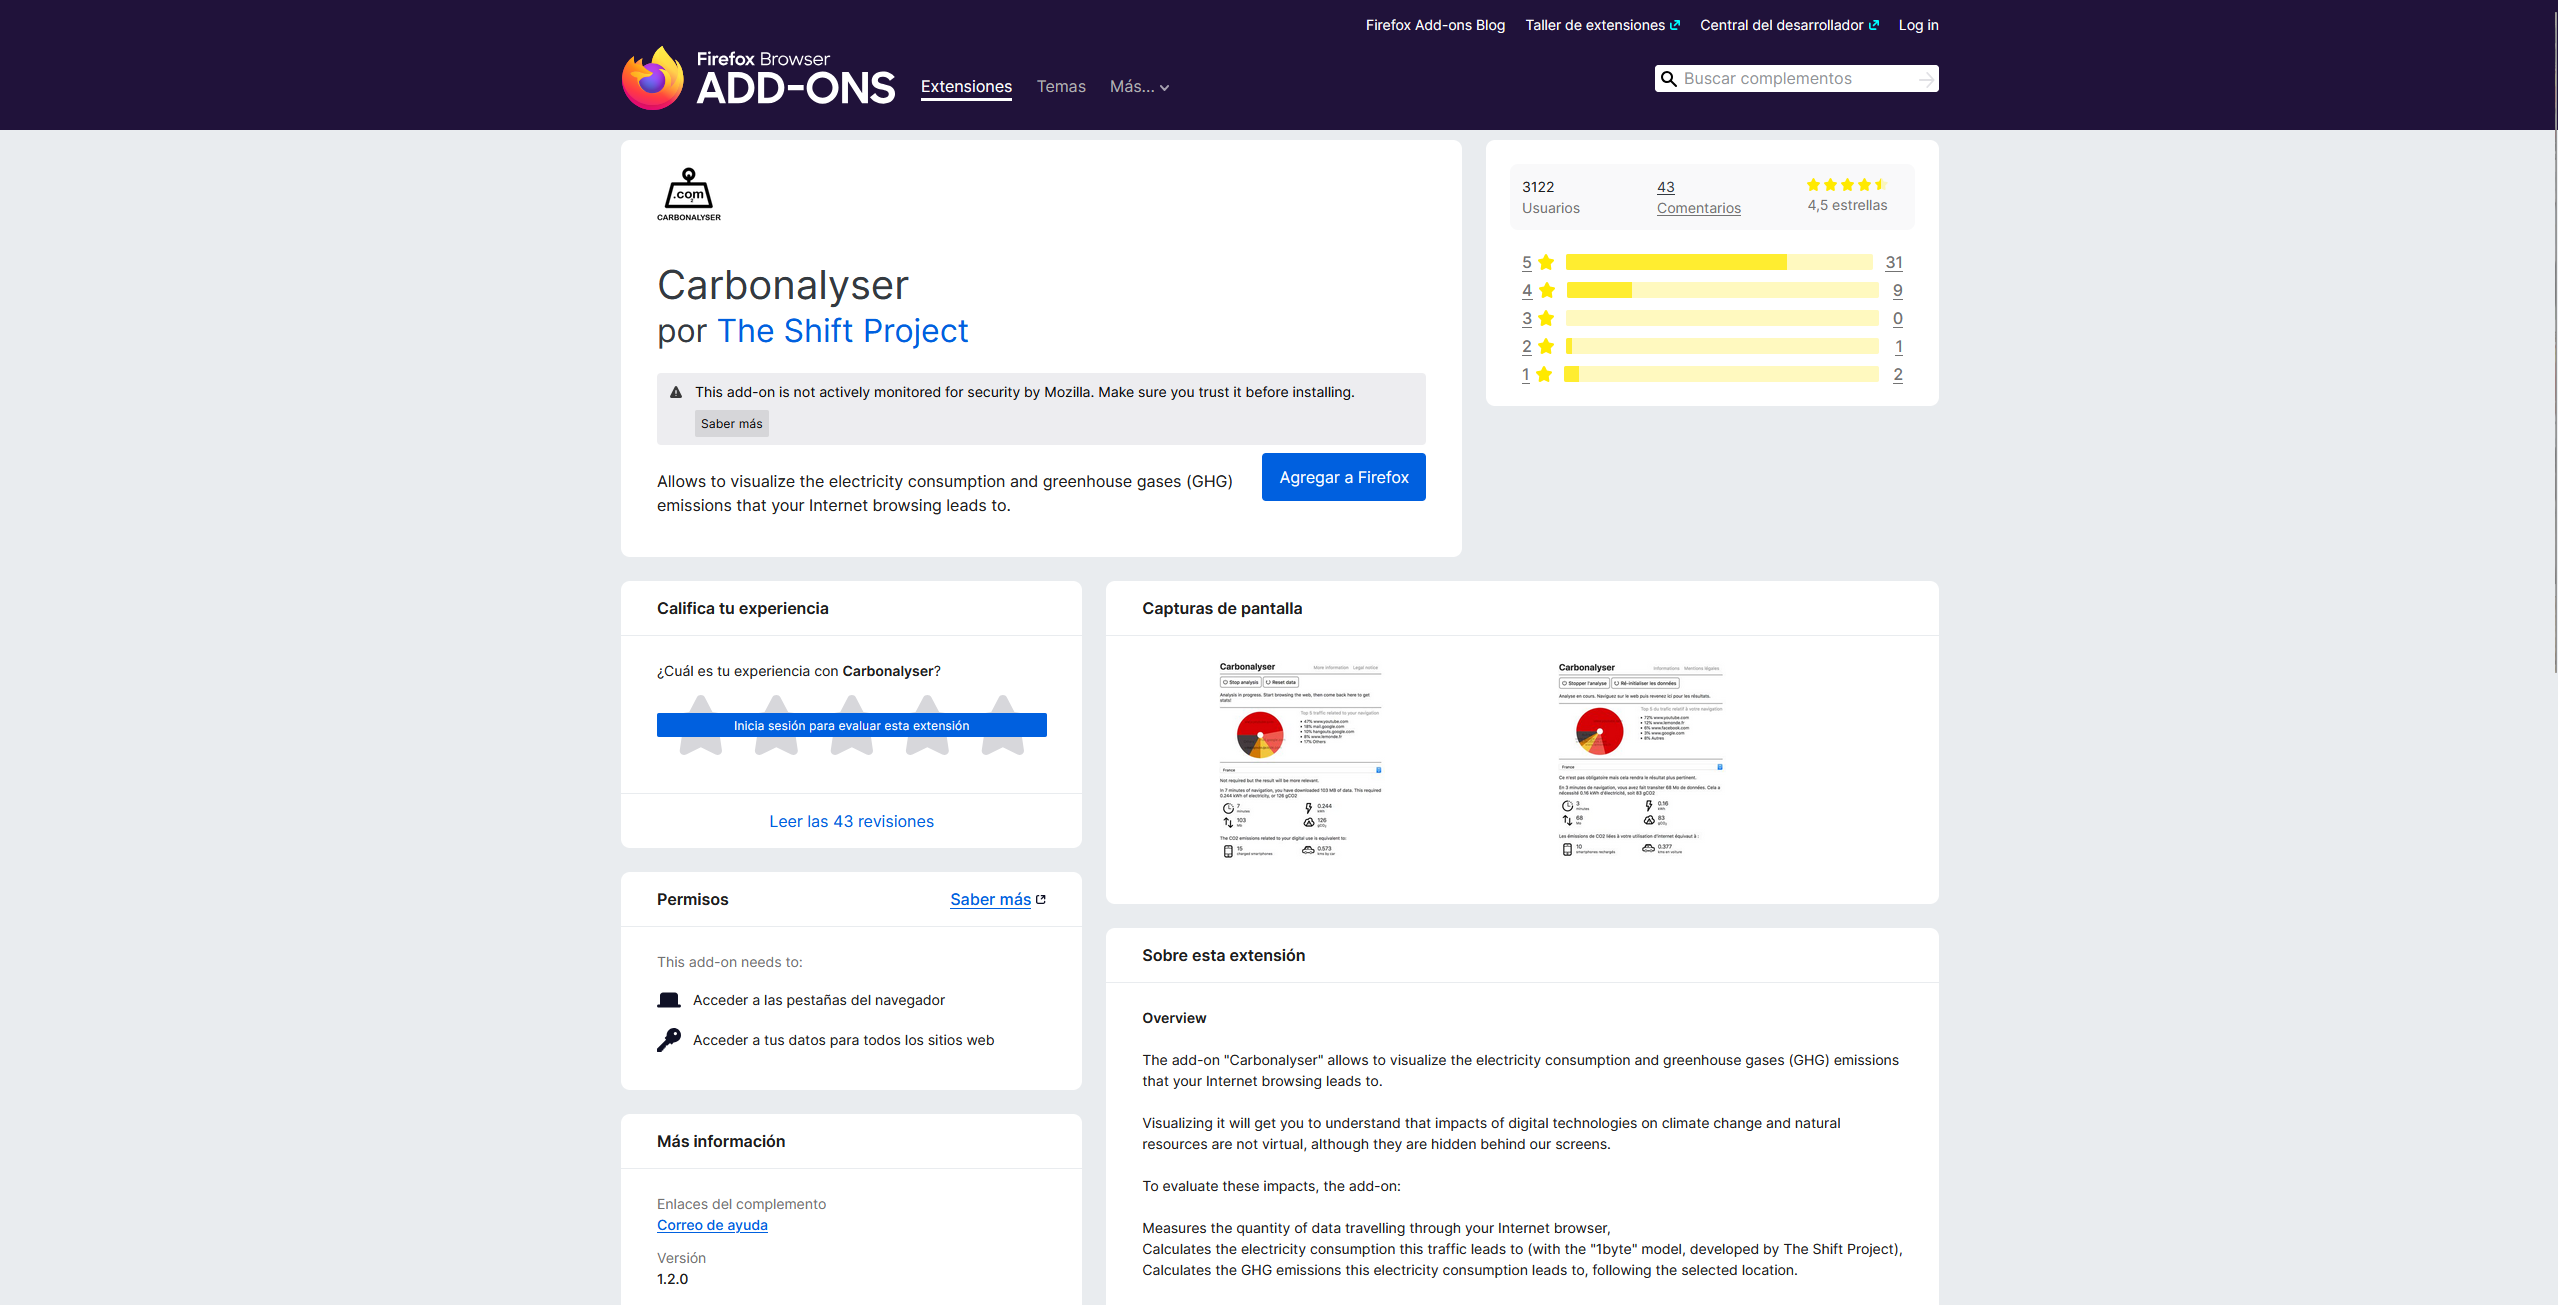
\includegraphics[width=0.8\textwidth]{imagenes/Carbonalyser_1.png}
  \captionof{figure}{Instalación de Carbonalyser en Firefox}
\end{center}

Una vez instalada podremos iniciar un análisis que analizará nuestra actividad
en el navegador a partir de ese punto.

\begin{center}
  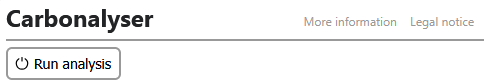
\includegraphics[width=0.8\textwidth]{imagenes/Carbonalyser_2.png}
  \captionof{figure}{Interfaz de monitorización de Carbonalyser}
\end{center}

Una vez hemos terminado, volvemos e indicamos nuestra región y con esto nos
dirá toda la información relevante en relación al análisis.

\begin{center}
  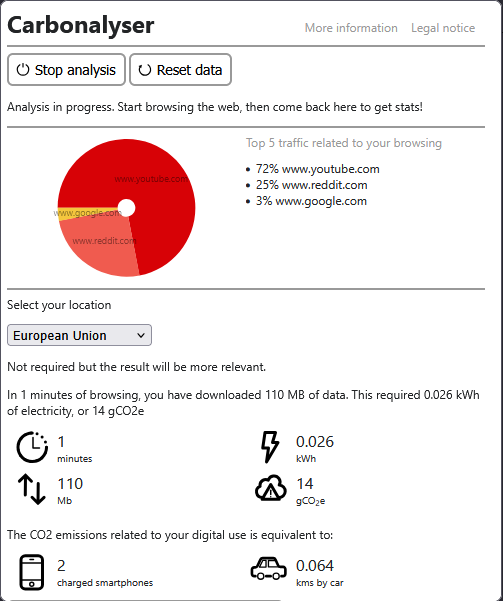
\includegraphics[width=0.8\textwidth]{imagenes/Carbonalyser_3.png}
  \captionof{figure}{Resultados del análisis de emisiones}
\end{center}

\subsection{Greenframe}
La forma más accesible y recomendada para comenzar con \textbf{GreenFrame} es a
través de su interfaz web.

\begin{center}
  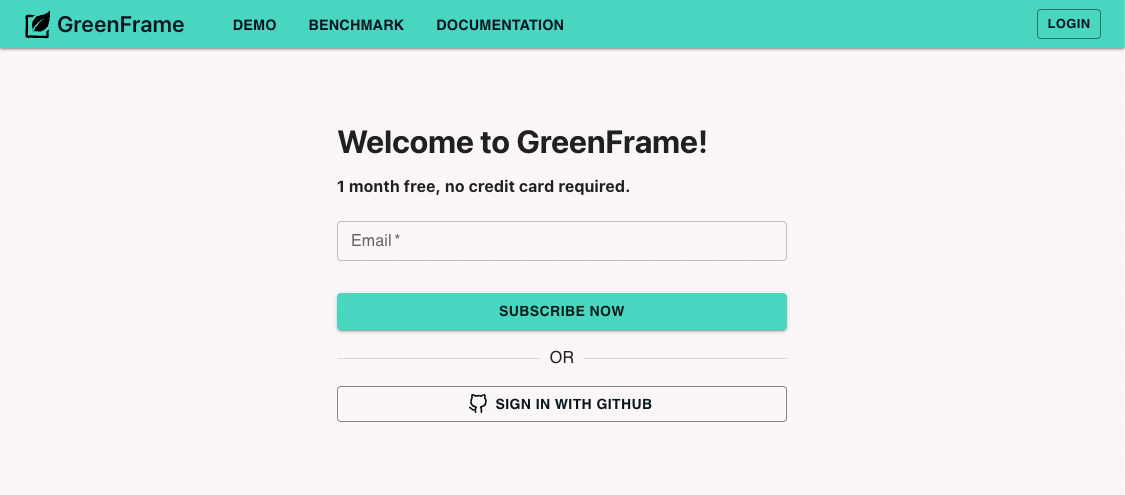
\includegraphics[width=0.9\textwidth]{imagenes/Greenframe_1.png}
\end{center}

Tras crear una cuenta gratuita (1 mes), puedes iniciar un proyecto y elegir
entre dos tipos de análisis: \textbf{"Single page"} y \textbf{"Full stack"}. El
tipo \textit{Single page} está pensado para medir el impacto ambiental de una
visita a una página web concreta, como por ejemplo una
\textbf{landing}\footnote{Página de aterrizaje web diseñada para recibir
  visitas y provocar una acción específica, como registrarse o comprar.} o una
página de inicio. Es ideal para casos sencillos y rápidos de analizar. Por otro
lado, la opción \textit{Full stack} permite definir escenarios más complejos,
simulando acciones del usuario en varias páginas e incluyendo la medición del
comportamiento del servidor (como contenedores Docker), ofreciendo una visión
más completa de la huella digital de toda la aplicación.

\begin{center}
  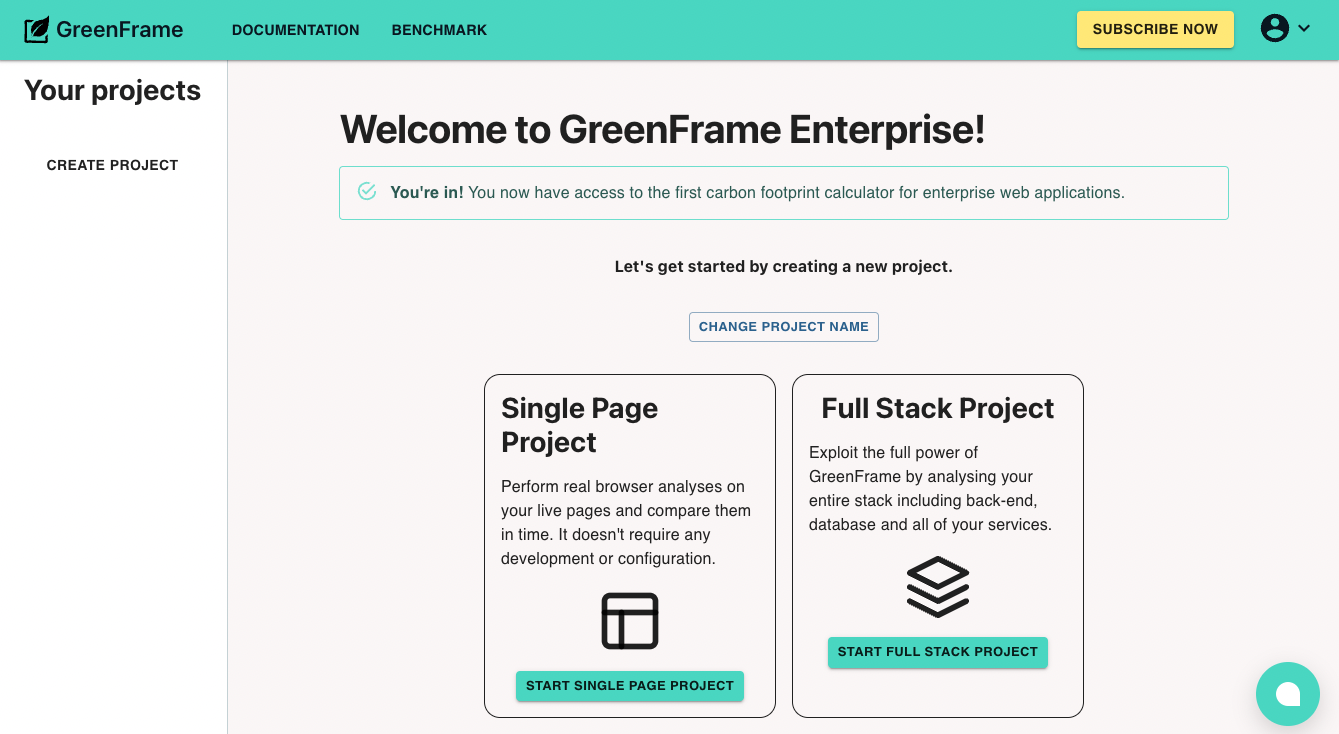
\includegraphics[width=0.9\textwidth]{imagenes/Greenframe_2.png}
\end{center}

Una vez que defines el tipo de proyecto e introduces la URL a analizar,
\textbf{GreenFrame simula tres visitas reales al sitio} usando un navegador en
la nube. Durante estas visitas registra múltiples métricas: uso de CPU, tráfico
de red, consumo de memoria y tiempo de carga. Esto le permite calcular de forma
más precisa las \textbf{emisiones estimadas de CO$_2$ equivalente (gCO$_2$e)}
que produce la interacción simulada.

\begin{center}
  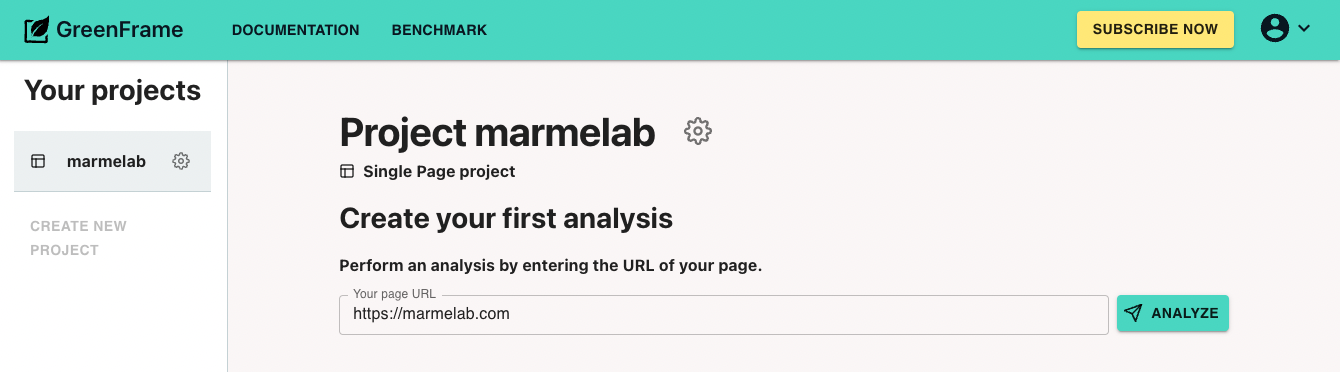
\includegraphics[width=0.9\textwidth]{imagenes/Greenframe_3.png}
\end{center}

\begin{center}
  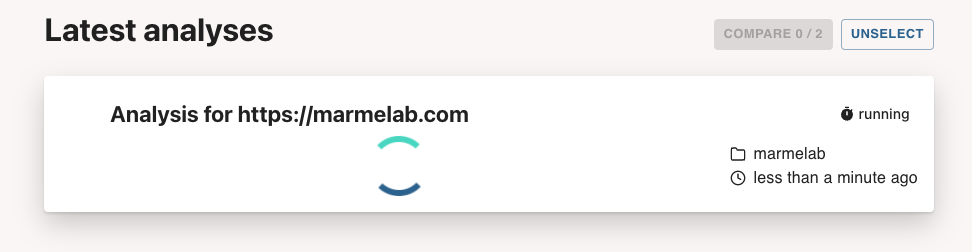
\includegraphics[width=0.9\textwidth]{imagenes/Greenframe_4.png}
\end{center}

Cuando el análisis finaliza (puede tardar unos minutos), se muestran los
resultados en una vista gráfica e interactiva. Se incluye un resumen con la
cantidad total de emisiones generadas y un \textbf{desglose por componentes y
  etapas del escenario}. Puedes examinar el comportamiento temporal de cada
componente (por ejemplo, el navegador), accediendo a una línea de tiempo que
detalla cómo y cuándo se generaron las emisiones durante la visita.

\begin{center}
  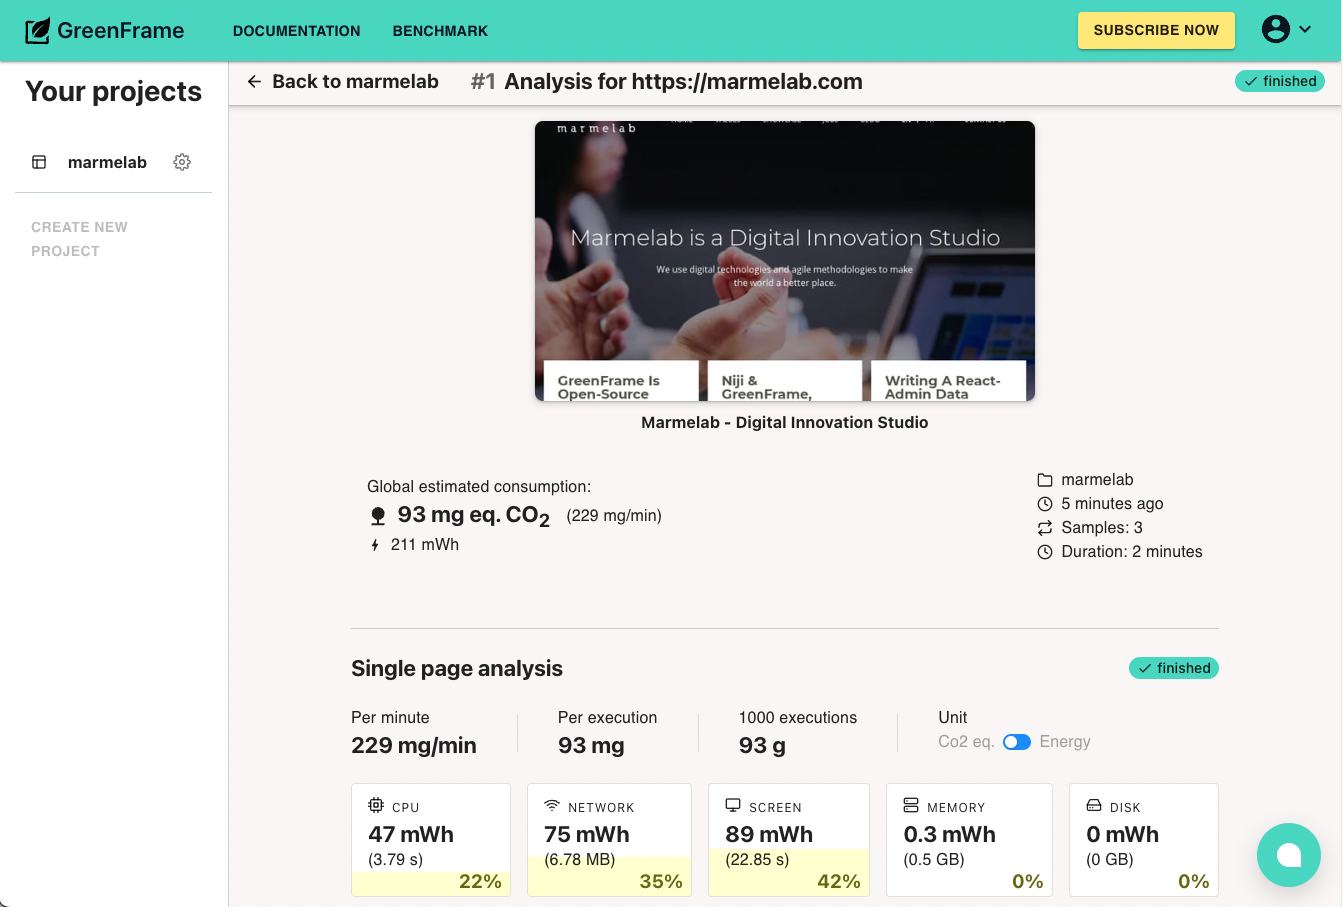
\includegraphics[width=0.9\textwidth]{imagenes/Greenframe_5.png}
\end{center}

\begin{center}
  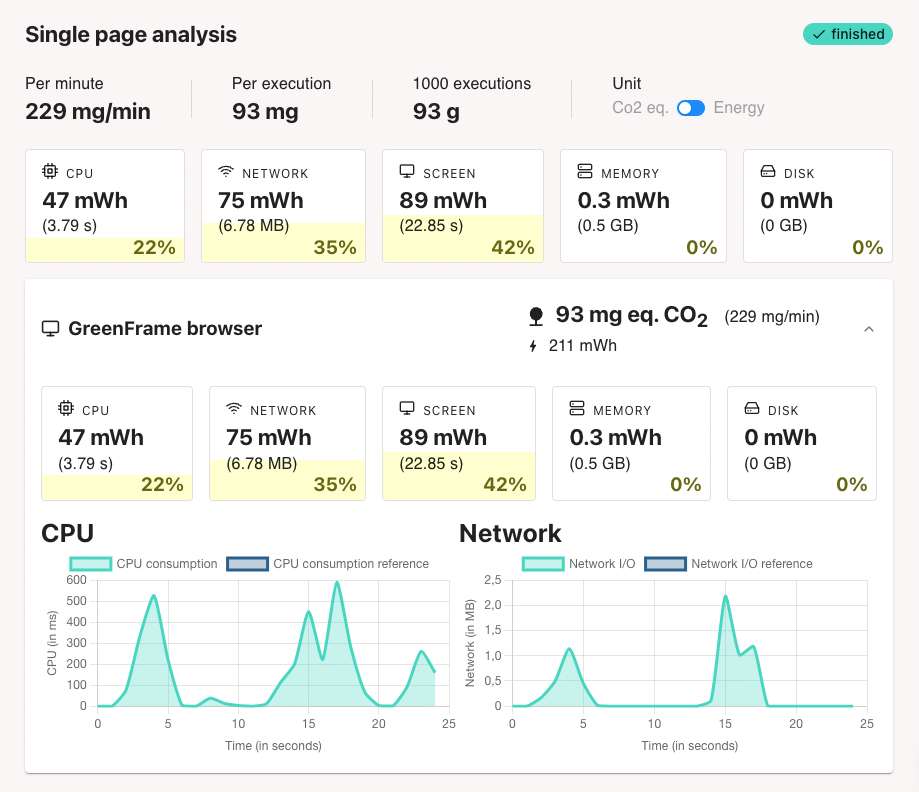
\includegraphics[width=0.9\textwidth]{imagenes/Greenframe_6.png}
\end{center}

Además, GreenFrame permite comparar diferentes análisis realizados sobre la
misma página o en distintas versiones del sitio. Esto es útil para evaluar si
los cambios en el código o contenido han reducido (o aumentado) el impacto
ambiental. El sistema te avisa si las diferencias entre análisis son mínimas y
podrían no ser significativas.

\begin{center}
  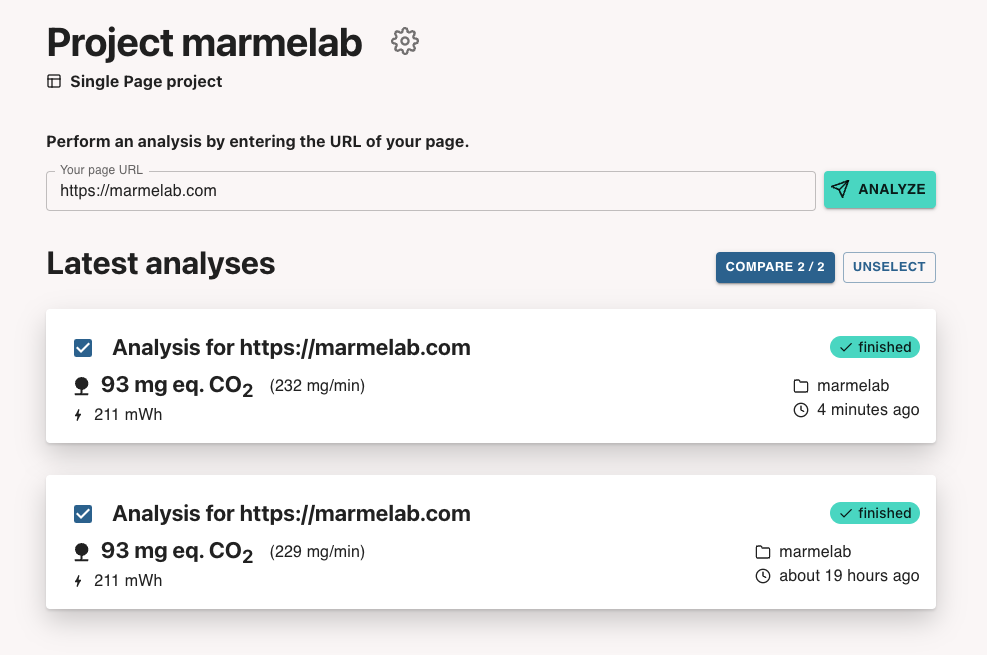
\includegraphics[width=0.9\textwidth]{imagenes/Greenframe_7.png}
\end{center}

\begin{center}
  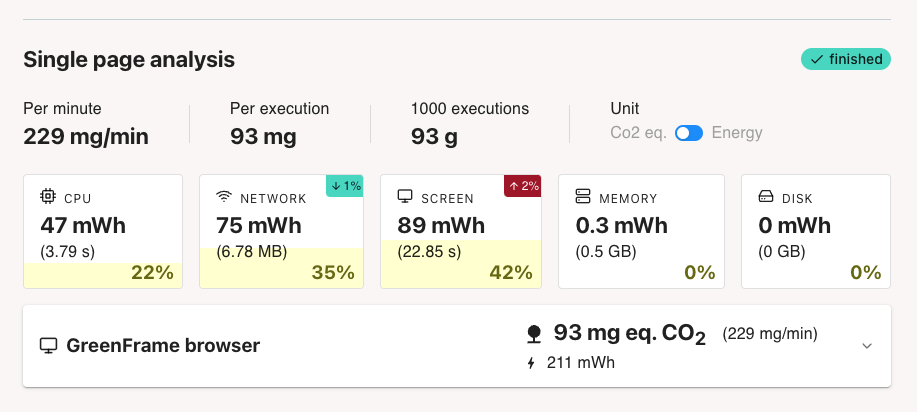
\includegraphics[width=0.9\textwidth]{imagenes/Greenframe_8.png}
\end{center}

Además, puedes usar \textbf{GreenFrame desde la terminal con su CLI}, o
integrarlo en un \textbf{pipeline de integración continua
  (CI}\footnote{(Continuous Integration) Técnica de desarrollo que automatiza la
  integración de código mediante pruebas continuas.}) para análisis
automatizados. Estas opciones son más potentes para desarrolladores que buscan
incorporar la sostenibilidad en sus flujos de trabajo.

\subsection{Website Carbon Calculator}
La forma más sencilla y recomendada de utilizar Website Carbon Calculator es a
través de su interfaz web.

\begin{center}
  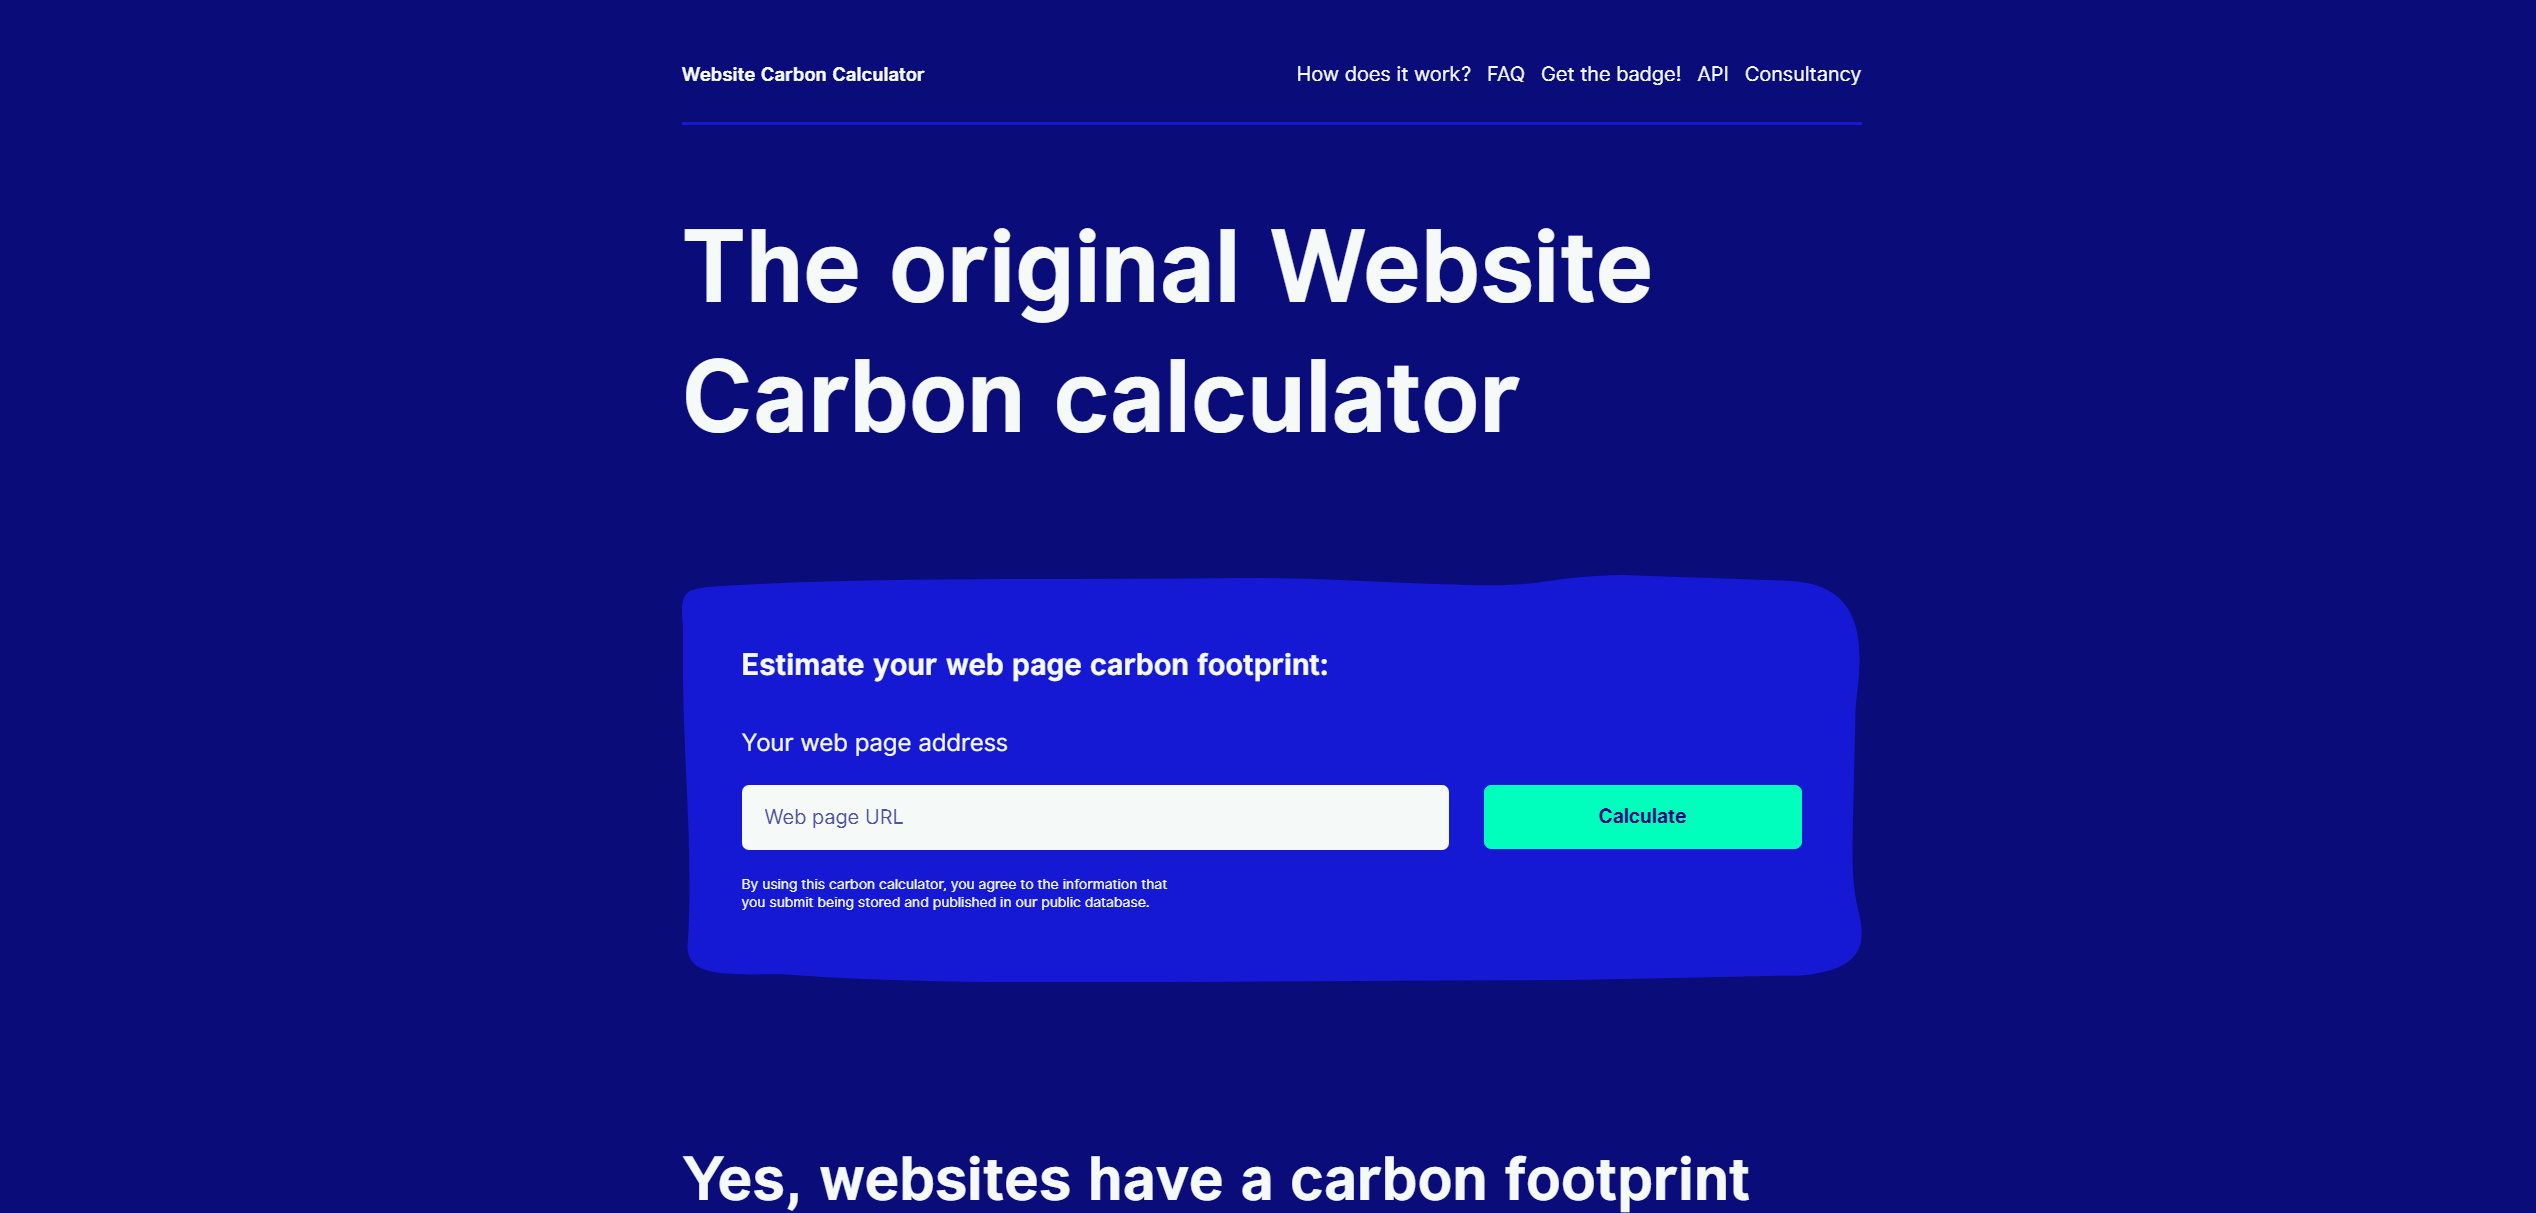
\includegraphics[width=0.7\textwidth]{imagenes/WCC_1.png}
\end{center}

Al introducir la URL del sitio web a analizar, la herramienta realiza las
siguientes acciones:

\begin{itemize}
  \item Mide el volumen de datos transferidos al cargar la página.
  \item Aplica un \textbf{factor de energía promedio por byte}\footnote{Estimación de
          energía consumida al transferir datos en internet, considerando red, servidores
          y dispositivos.}, considerando el consumo en el dispositivo del usuario, la red
        y el centro de datos.
  \item Consulta la base de datos de la \textbf{Green Web
          Foundation}\footnote{Organización que mantiene una base de datos sobre si los
          proveedores usan energía renovable.} para saber si el proveedor de alojamiento
        usa energía renovable.
  \item Convierte el consumo energético estimado (en kWh) en emisiones de CO$_2$e
        utilizando factores de conversión basados en la fuente de energía.
\end{itemize}

El resultado del análisis incluye:

\begin{itemize}
  \item \textbf{Emisiones estimadas por visita} (en gCO$_2$e).
  \item Comparación con el \textbf{promedio global} (\textasciitilde0.8
        gCO$_2$e/vista).
  \item \textbf{Porcentaje ''cleanerThan''}\footnote{Métrica que indica el porcentaje de sitios web más contaminantes que el analizado.}: indica qué proporción de sitios analizados son más contaminantes que el tuyo.
  \item Estimación anual de emisiones basada en el número de visitas.
\end{itemize}

\begin{center}
  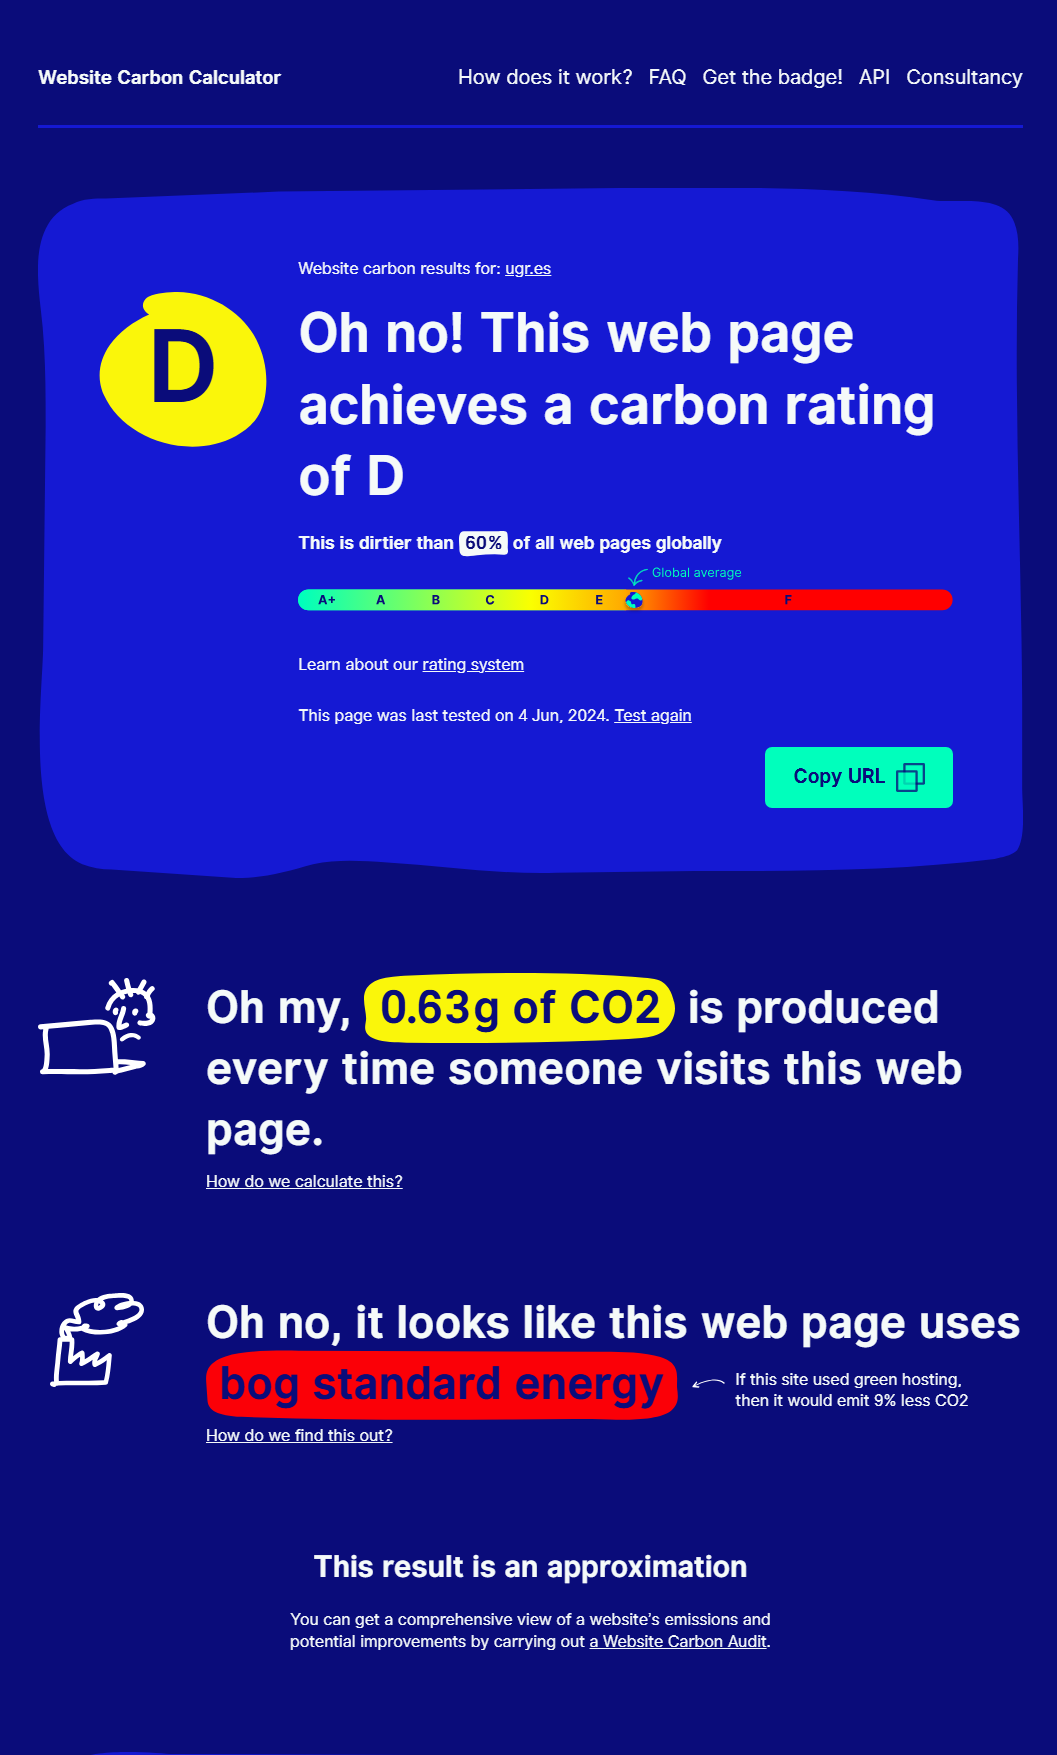
\includegraphics[width=0.7\textwidth]{imagenes/WCC_2.png}
\end{center}

\begin{center}
  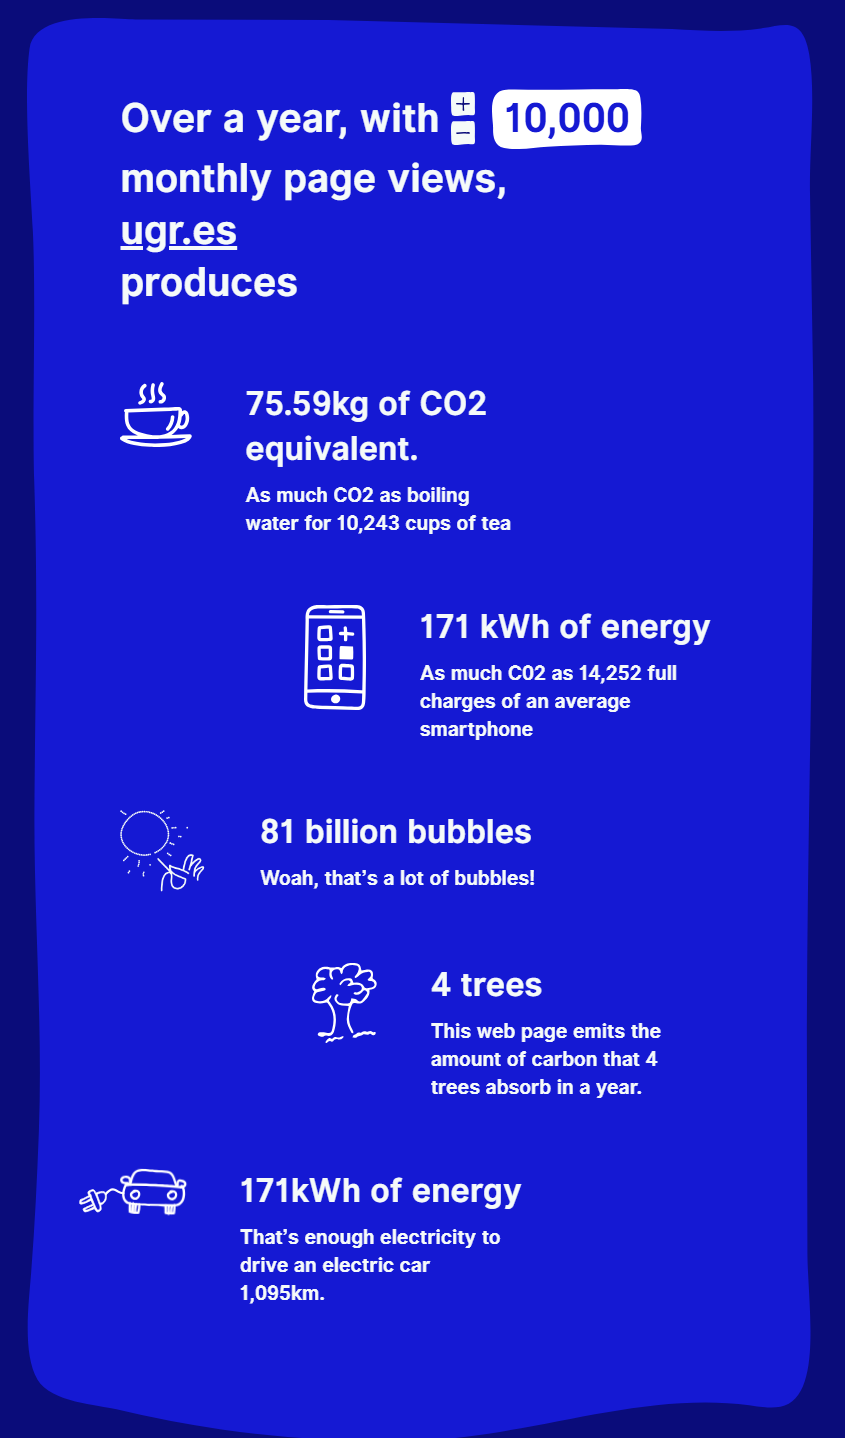
\includegraphics[width=0.7\textwidth]{imagenes/WCC_3.png}
\end{center}

\subsection{Ecograder}
Para usarlo solo necesitaremos entrar en su web \url{https://ecograder.com/} y
introducir la URL de la web que queremos analizar.

\begin{center}
  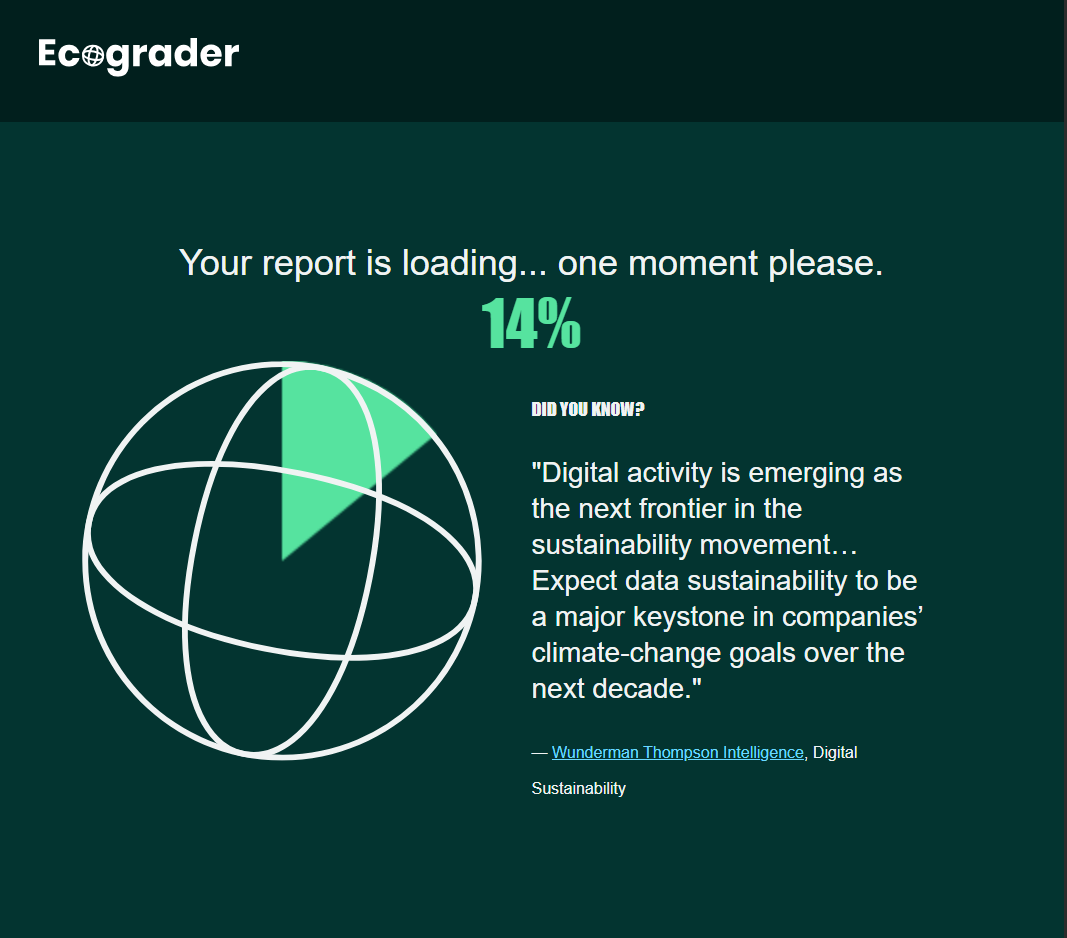
\includegraphics[width=0.9\textwidth]{imagenes/Ecograder_1.png}
\end{center}

ECOGrader lanzará un análisis que combina
\textbf{Lighthouse}\footnote{Herramienta automatizada de Google que audita el
  rendimiento, accesibilidad y buenas prácticas de páginas web.} y
\textbf{CO2.js} para estimar las emisiones de CO$_2$ equivalente (gCO$_2$e).
\textbf{CO2.js} calcula emisiones según cuatro segmentos: dispositivo de
usuario, red, centro de datos (usando datos de la red eléctrica regional, según
la \textbf{intensidad de carbono regional}) y producción de hardware. Además, integra datos de
intensidad de carbono por región y detecta si el sitio está alojado en un
proveedor "\textbf{hosting verde}"\footnote{Servicio de alojamiento web
  alimentado total o parcialmente por fuentes de energía renovables.}. Por su
parte, \textbf{Lighthouse} aporta métricas de rendimiento como "\textbf{First
  Contentful Paint (FCP)}"\footnote{Métrica de Lighthouse que mide el tiempo
  hasta que el primer contenido se renderiza en pantalla.} o "\textbf{Time to
  Interactive (TTI)}"\footnote{Métrica de Lighthouse que indica cuándo una página
  se vuelve completamente interactiva para el usuario.}, que ECOGrader adapta
para generar recomendaciones de optimización.

\begin{center}
  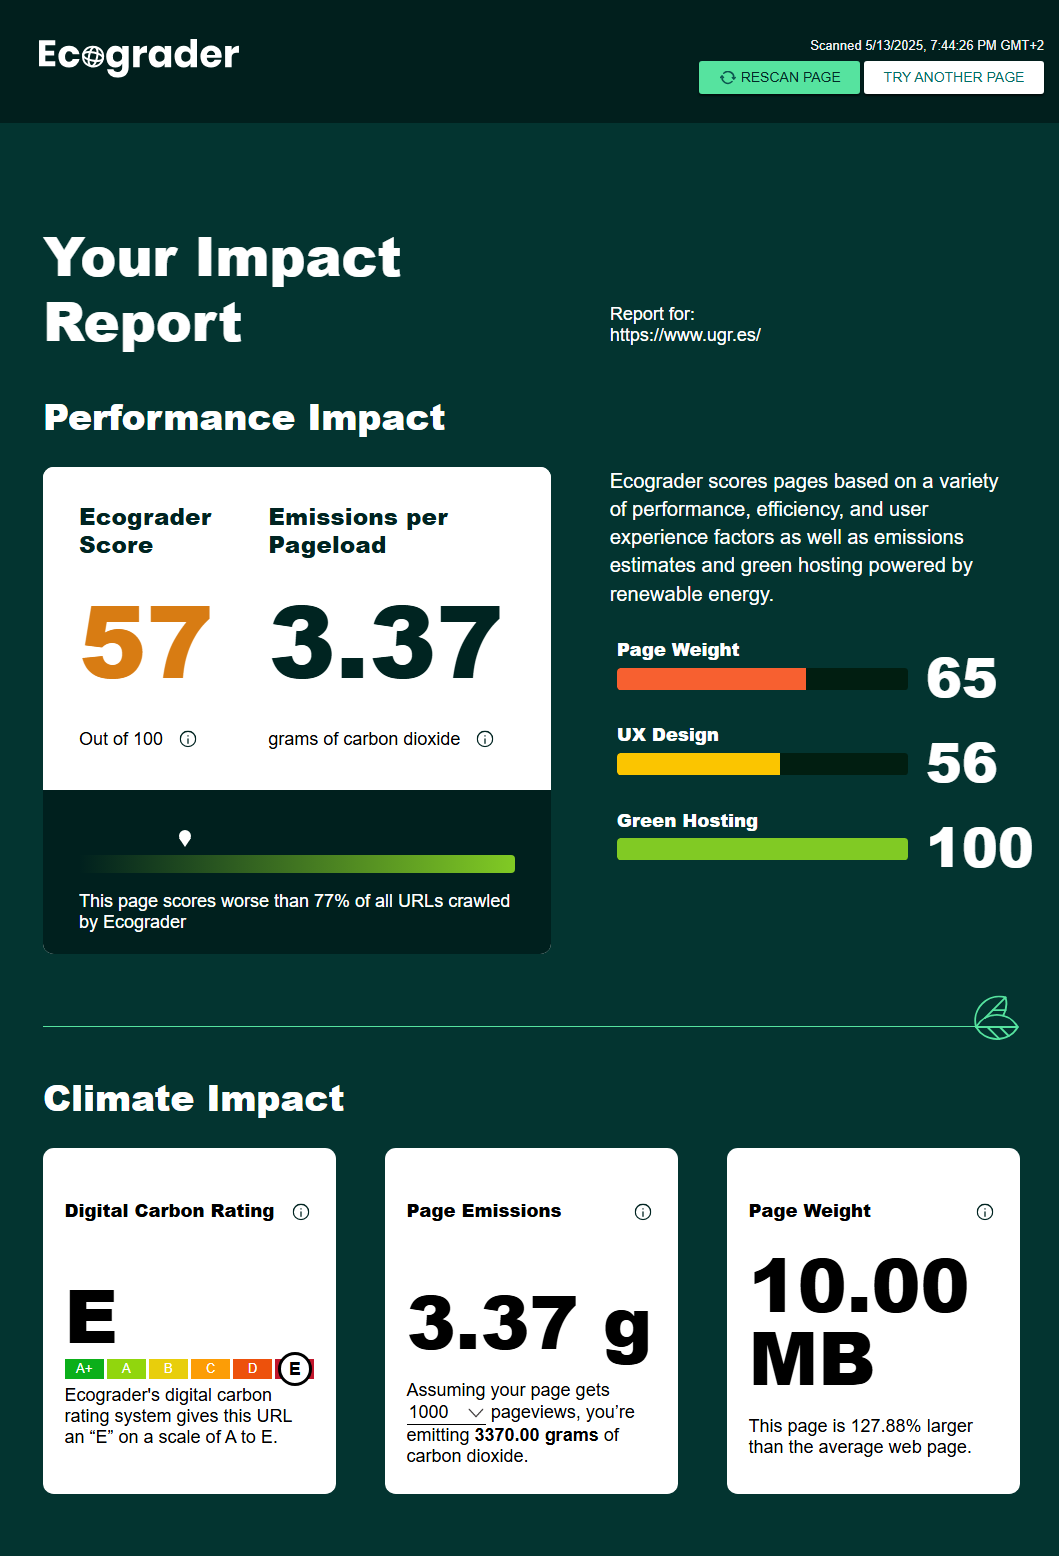
\includegraphics[width=0.9\textwidth]{imagenes/Ecograder_2.png}
\end{center}

\begin{center}
  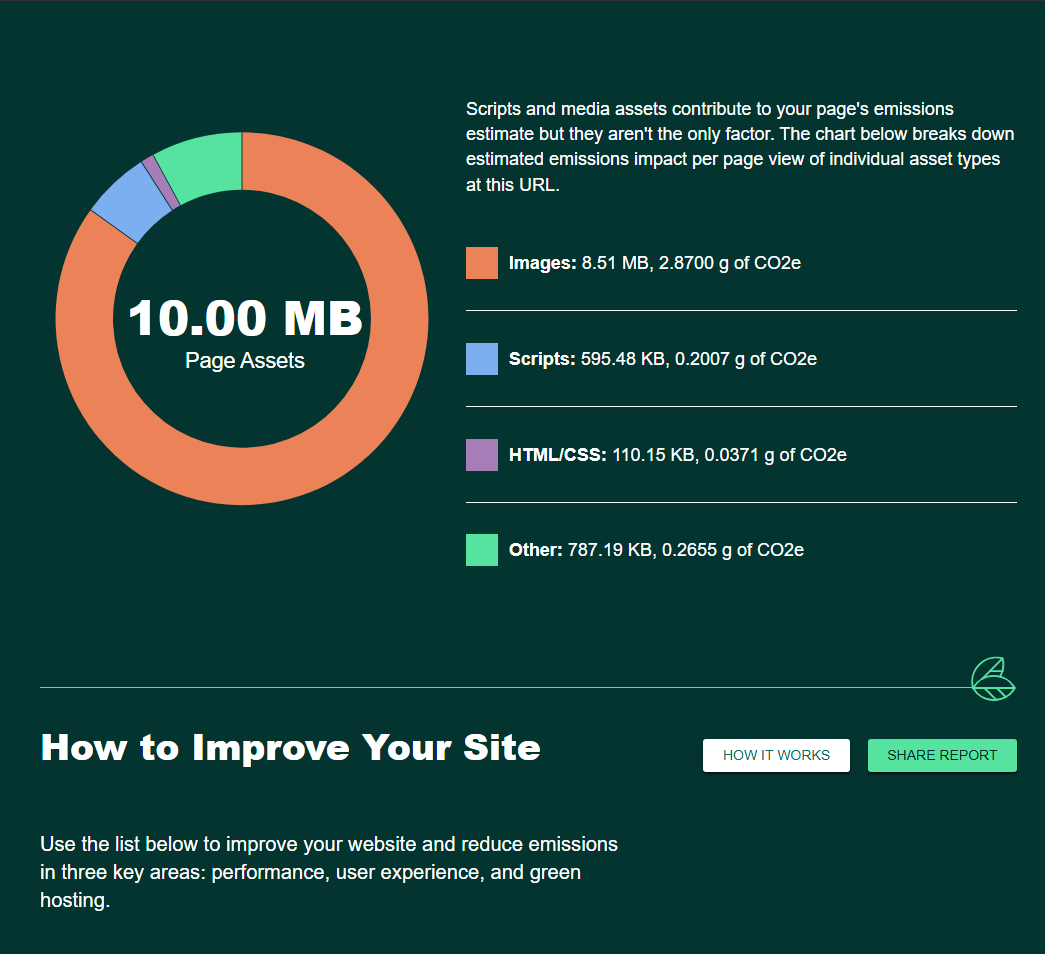
\includegraphics[width=0.9\textwidth]{imagenes/Ecograder_3.png}
\end{center}

\begin{center}
  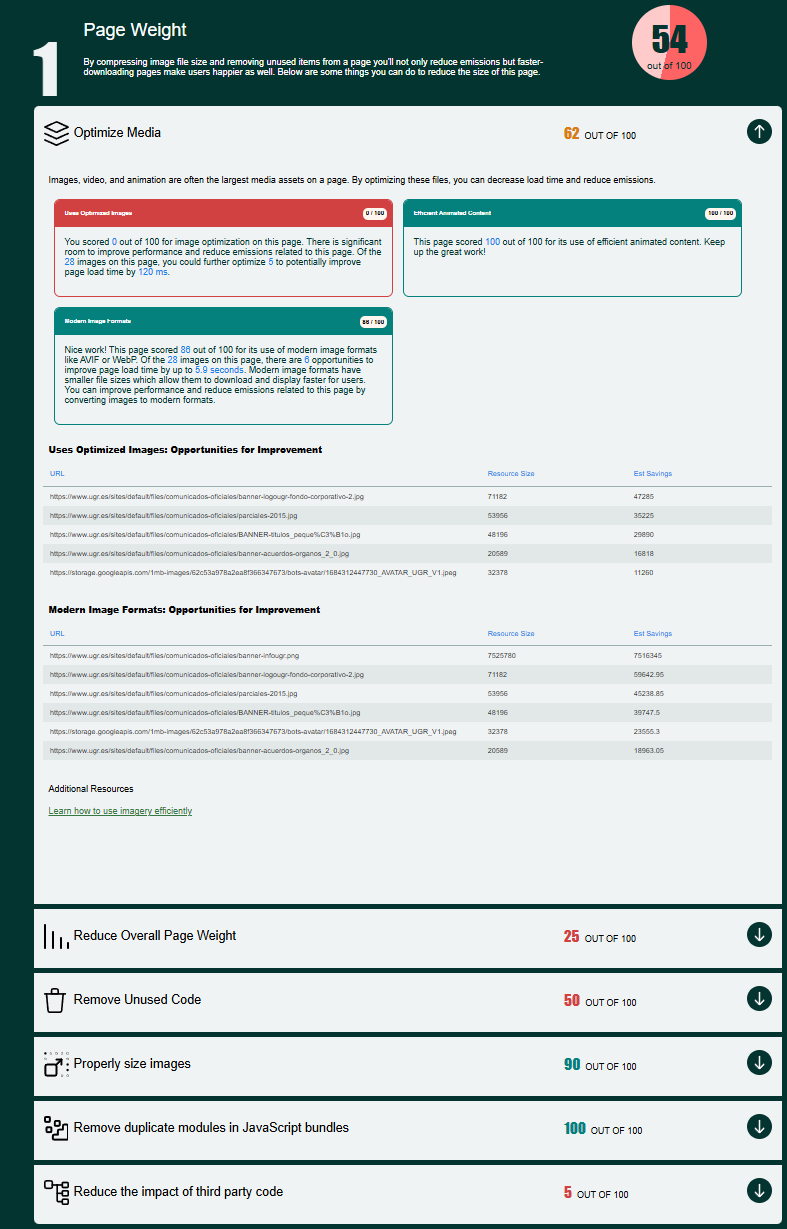
\includegraphics[width=0.9\textwidth]{imagenes/Ecograder_4.png}
\end{center}

\begin{center}
  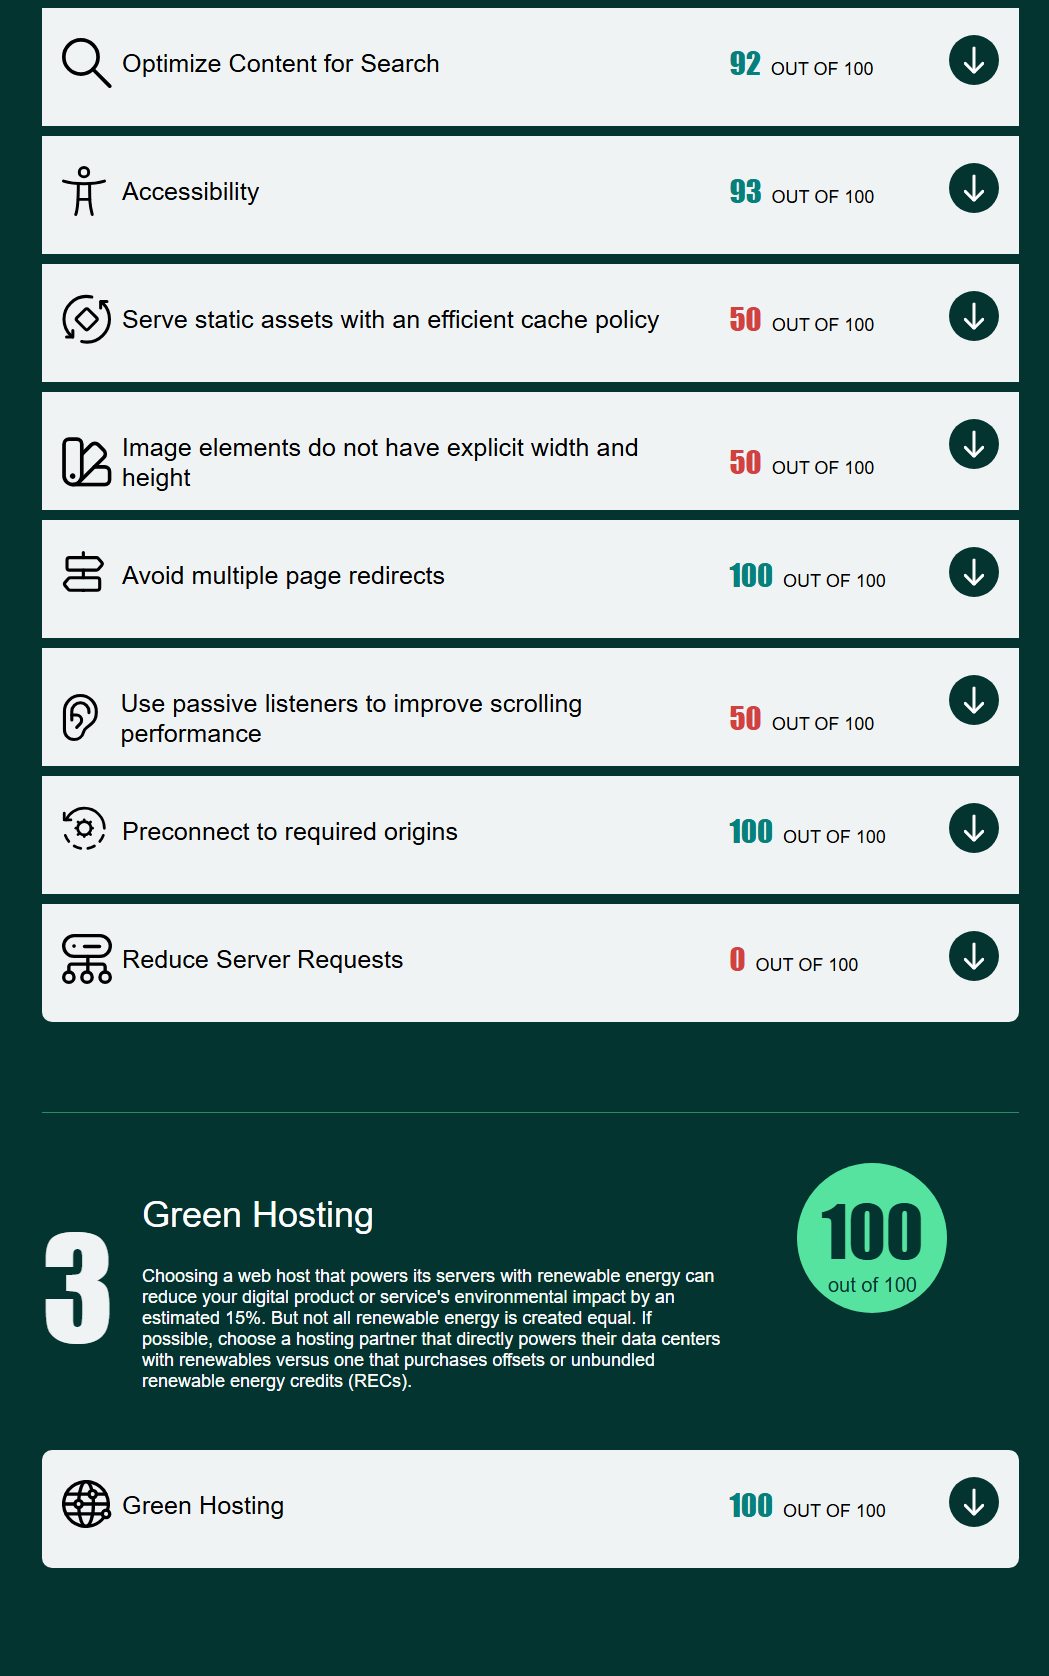
\includegraphics[width=0.9\textwidth]{imagenes/Ecograder_5.png}
\end{center}

\subsection{CodeCarbon}
Para poder usarlo en nuestros proyectos instalaremos el paquete de Python
usando los gestores de paquete \textbf{pip}\footnote{Herramienta para instalar
  y gestionar paquetes de Python.} o \textbf{conda}\footnote{Gestor de entornos y
  paquetes, popular en ciencia de datos.}:

\begin{tcolorbox}[colback=codebackground, colframe=codeborder, boxrule=0.8pt, arc=0mm, boxsep=5pt, left=5pt, right=5pt, top=5pt, bottom=5pt]
  \begin{lstlisting}[language=bash]
    pip install codecarbon
  \end{lstlisting}
\end{tcolorbox}

Tras esto, usando el comando

\begin{tcolorbox}[colback=codebackground, colframe=codeborder, boxrule=0.8pt, arc=0mm, boxsep=5pt, left=5pt, right=5pt, top=5pt, bottom=5pt]
  \begin{lstlisting}[language=bash]
    codecarbon config
  \end{lstlisting}
\end{tcolorbox}

se nos guiará a la hora de crear el archivo de configuración de nuestro
proyecto, en el que indicaremos datos como la región o si este se está
ejecutando en la nube.

A continuación ya podemos monitorear las emisiones de nuestro equipo sin
cambiar el código con:

\begin{tcolorbox}[colback=codebackground, colframe=codeborder, boxrule=0.8pt, arc=0mm, boxsep=5pt, left=5pt, right=5pt, top=5pt, bottom=5pt]
  \begin{lstlisting}[language=bash]
    codecarbon monitor
  \end{lstlisting}
\end{tcolorbox}

El cual enviará la información a una \textbf{API} alojada en
"localhost:8008".

\textbf{CodeCarbon} también permite medir emisiones usando un objeto \texttt{EmissionsTracker} con \texttt{start()} y \texttt{stop()}, ideal para bloques amplios de código:

\begin{tcolorbox}[colback=codebackground, colframe=codeborder, boxrule=0.8pt, arc=0mm, boxsep=5pt, left=5pt, right=5pt, top=5pt, bottom=5pt]
  \begin{lstlisting}[language=bash]
    from codecarbon import EmissionsTracker
    tracker = EmissionsTracker()
    tracker.start()
    try:
      #Codigo intensivo en computo aqui
      _ = 1 + 1
    finally:
      tracker.stop()
  \end{lstlisting}
\end{tcolorbox}

Y para secciones específicas puedes usar tareas con \texttt{start\_task()} /
\texttt{stop\_task()}:

\begin{tcolorbox}[colback=codebackground, colframe=codeborder, boxrule=0.8pt, arc=0mm, boxsep=5pt, left=5pt, right=5pt, top=5pt, bottom=5pt]
  \begin{lstlisting}[language=bash]
    try:
      tracker = EmissionsTracker(project_name="bert_inference", measure_power_secs=10)
      tracker.start_task("load dataset")
      dataset = load_dataset("imdb", split="test")
      imdb_emissions = tracker.stop_task()
      tracker.start_task("build model")
      model = build_model()
      model_emissions = tracker.stop_task()
    finally:
      _ = tracker.stop()
  \end{lstlisting}
\end{tcolorbox}

Otra opción es el uso como \textbf{gestor de contexto\textsuperscript{3}}:

\begin{tcolorbox}[colback=codebackground, colframe=codeborder, boxrule=0.8pt, arc=0mm, boxsep=5pt, left=5pt, right=5pt, top=5pt, bottom=5pt]
  \begin{lstlisting}[language=bash]
  from codecarbon import EmissionsTracker

  with EmissionsTracker() as tracker:
    # Codigo intensivo aqui
  \end{lstlisting}
\end{tcolorbox}

Y finalmente, si tu código está en una función, puedes decorarla con
\texttt{@track\_emissions}:

\begin{tcolorbox}[colback=codebackground, colframe=codeborder, boxrule=0.8pt, arc=0mm, boxsep=5pt, left=5pt, right=5pt, top=5pt, bottom=5pt]
  \begin{lstlisting}[language=bash]
  from codecarbon import track_emissions

  @track_emissions
  def training_loop():
    # Codigo de entrenamiento intensivo aqui
  \end{lstlisting}
\end{tcolorbox}

Además, dispones de dos formas de visualizar los datos recopilados:

\textbf{Offline}, con la herramienta \texttt{carbonboard}:

\begin{tcolorbox}[colback=codebackground, colframe=codeborder, boxrule=0.8pt, arc=0mm, boxsep=5pt, left=5pt, right=5pt, top=5pt, bottom=5pt]
  \begin{lstlisting}[language=bash]
  carbonboard --filepath="examples/emissions.csv" --port=3333
  \end{lstlisting}
\end{tcolorbox}

\begin{center}
  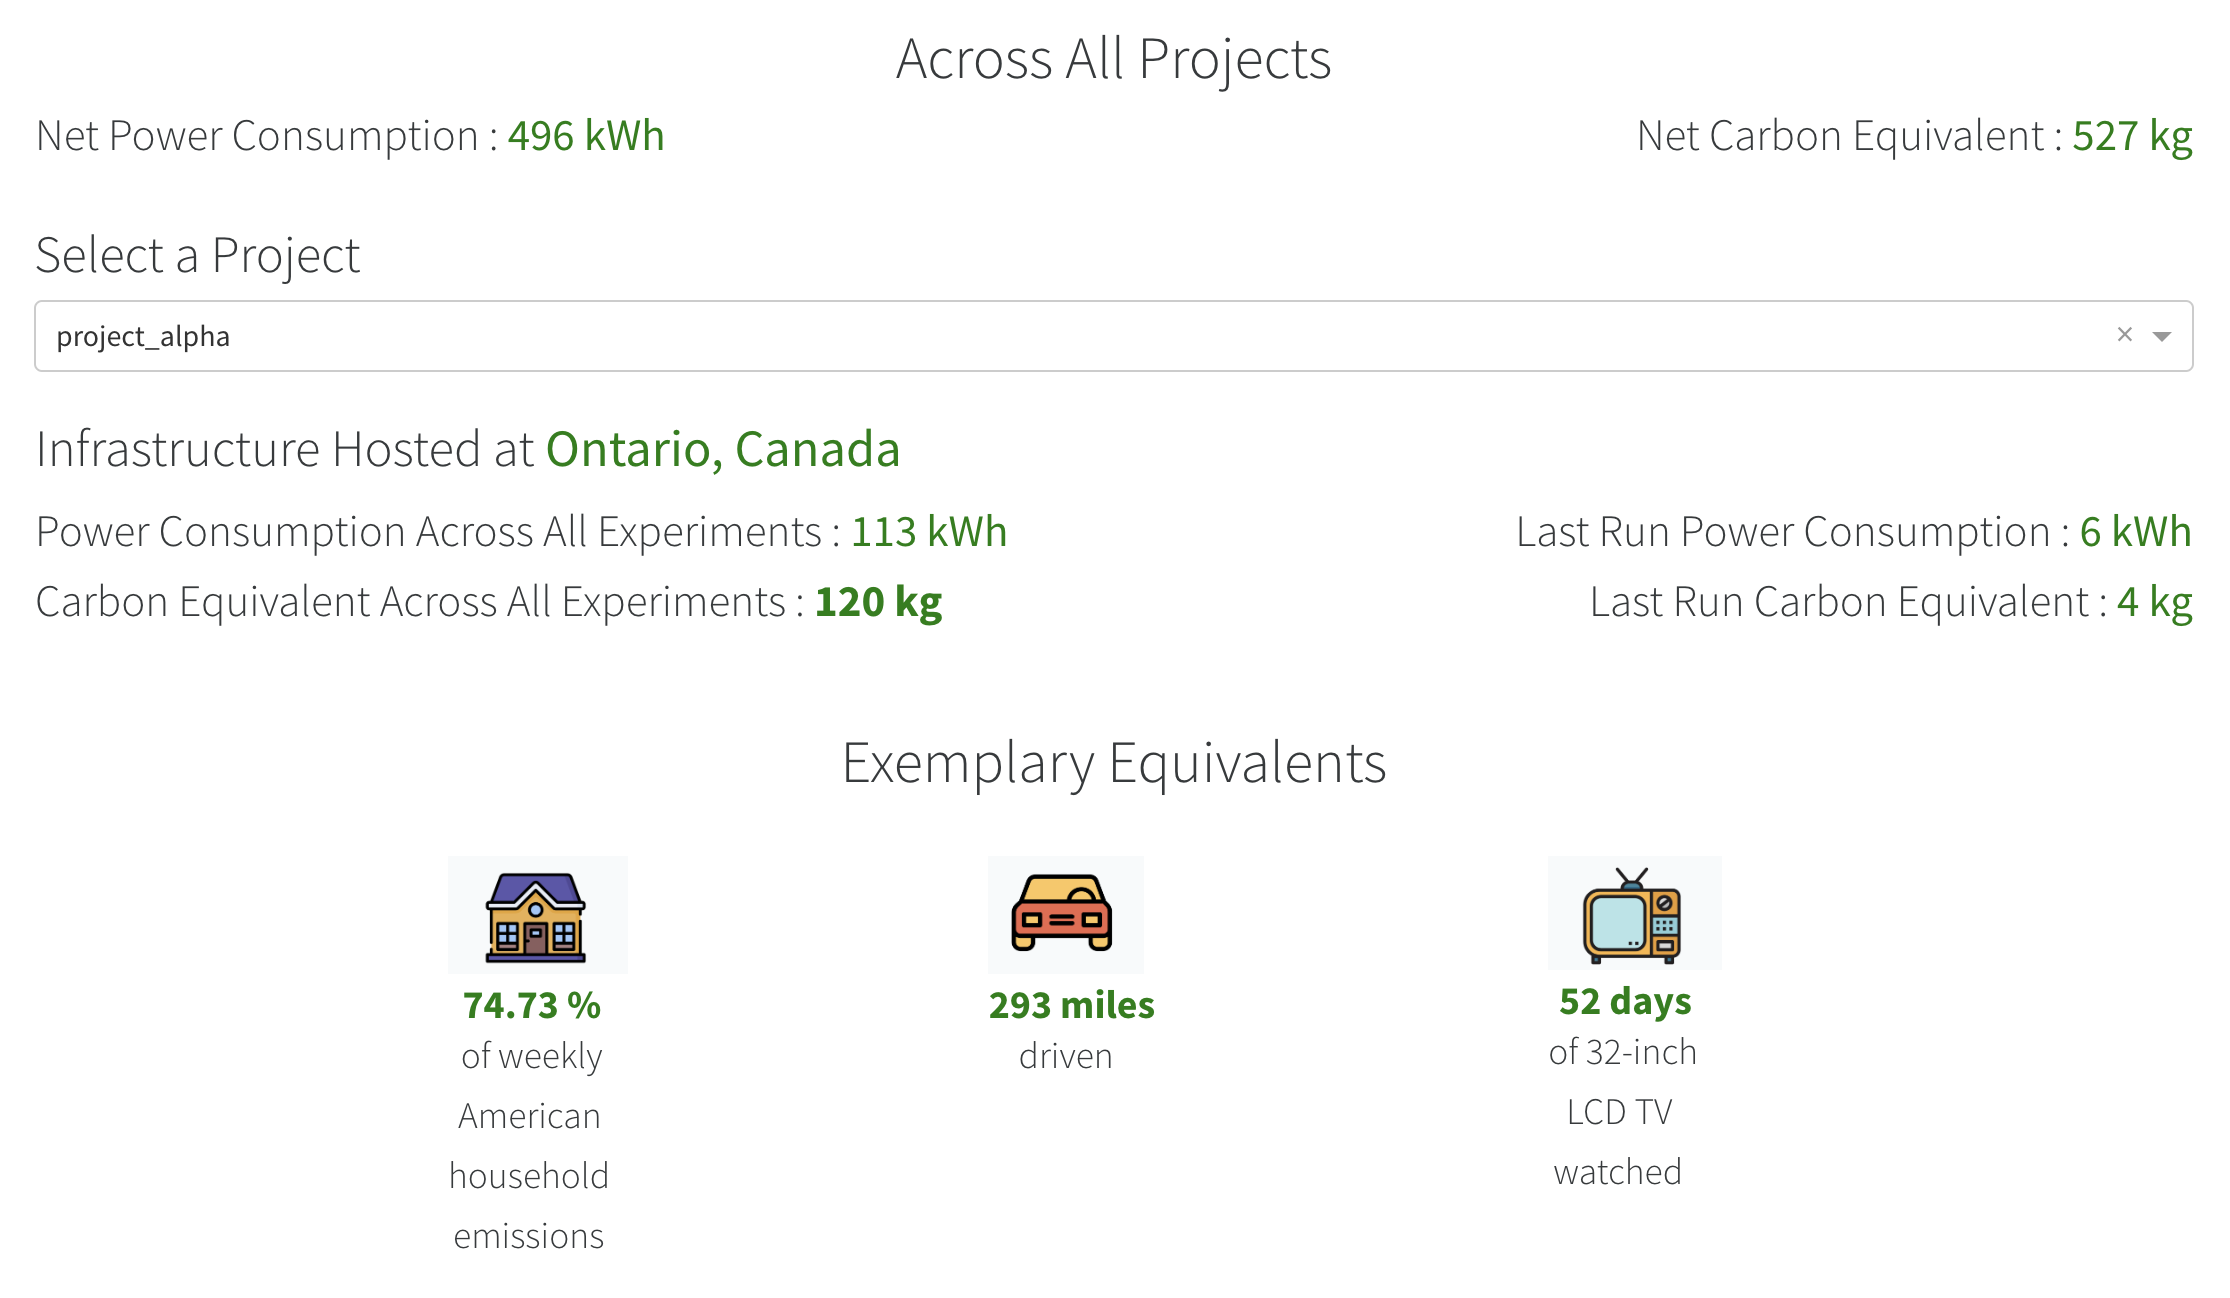
\includegraphics[width=0.9\textwidth]{imagenes/CC_1.png}
\end{center}

\begin{center}
  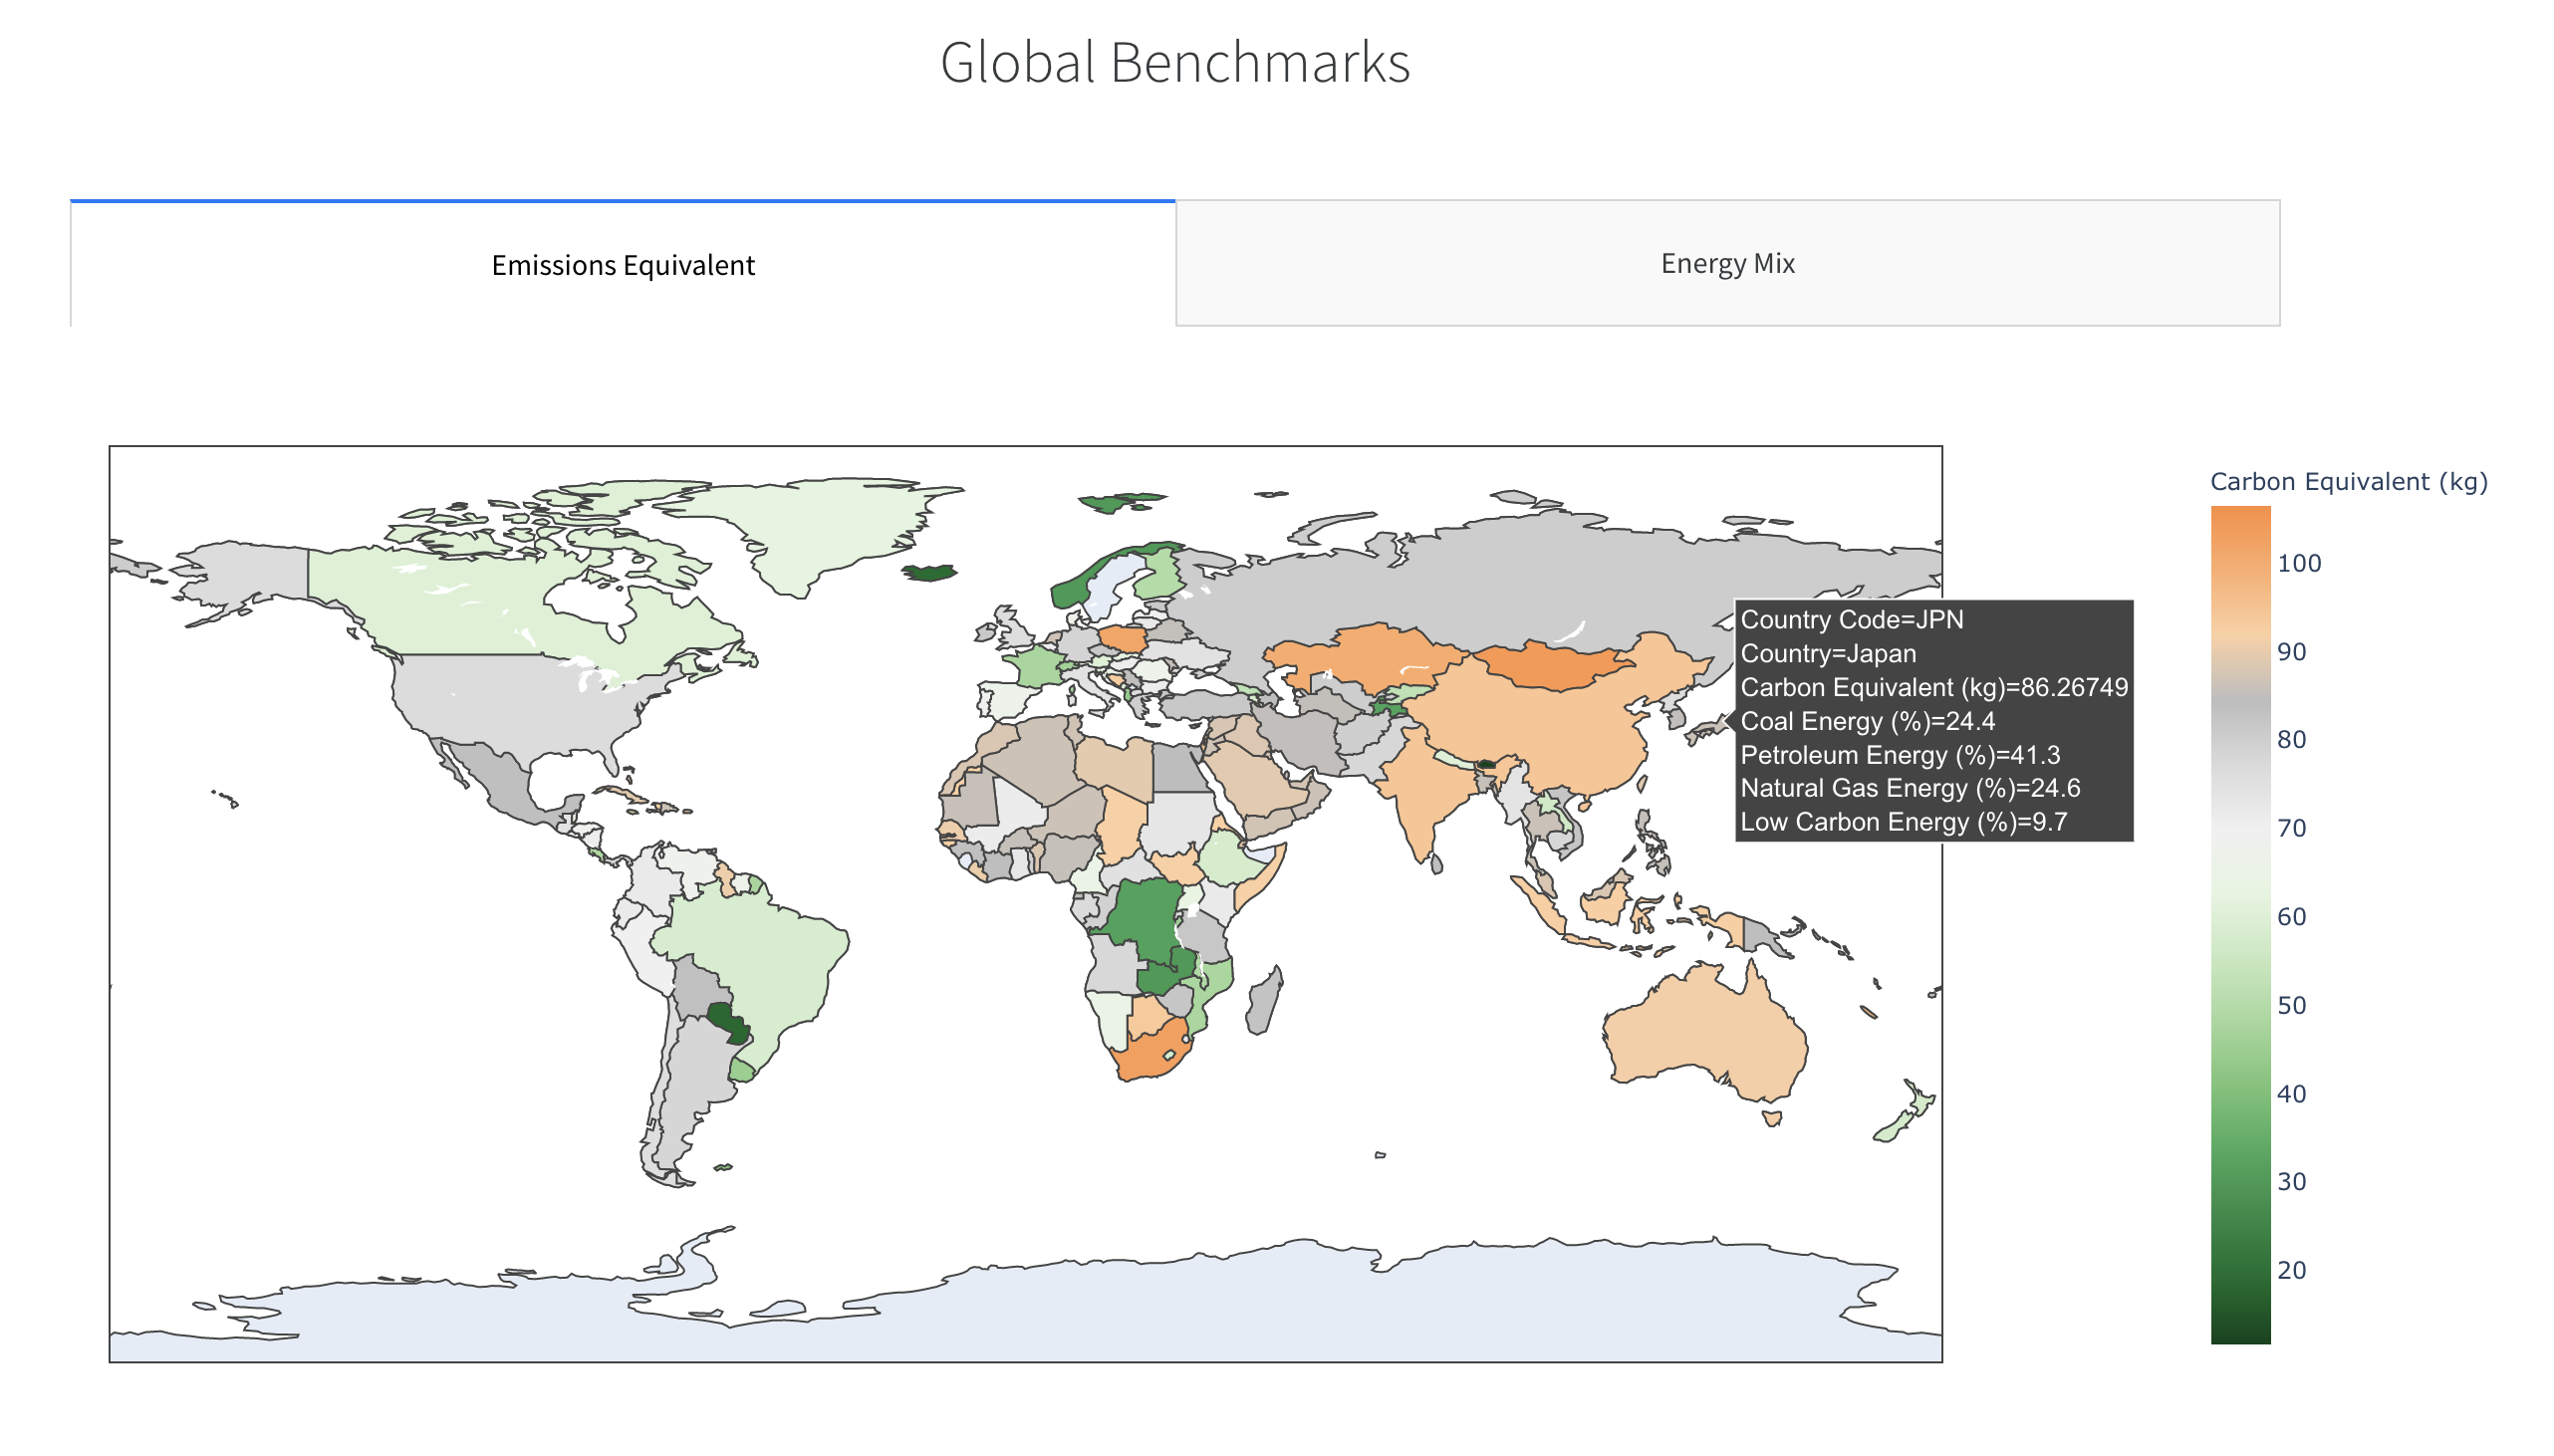
\includegraphics[width=0.9\textwidth]{imagenes/CC_2.png}
\end{center}

\textbf{Online}, si permites subir datos a la API pública de CodeCarbon, accediendo a un dashboard web:

\begin{center}
  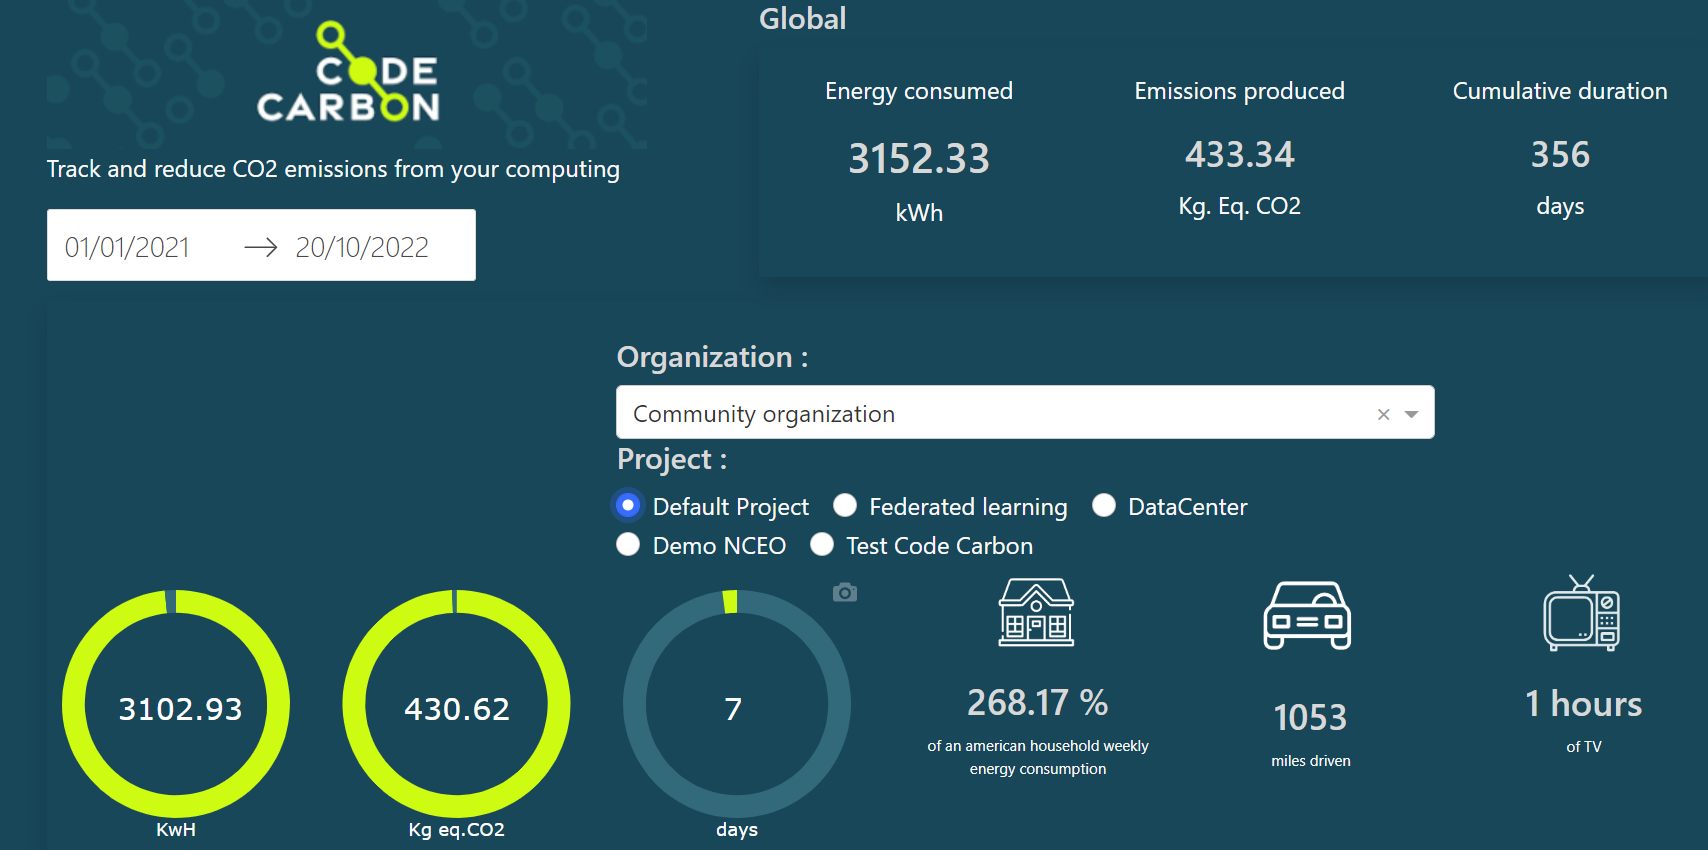
\includegraphics[width=0.9\textwidth]{imagenes/CC_3.png}
\end{center}

\begin{center}
  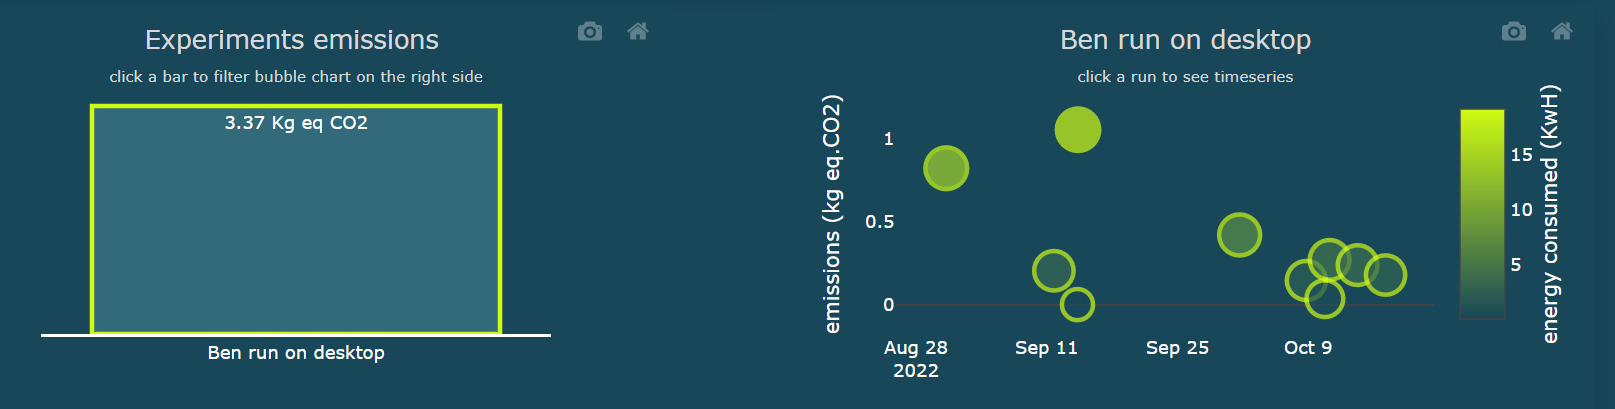
\includegraphics[width=0.9\textwidth]{imagenes/CC_4.png}
\end{center}

\begin{center}
  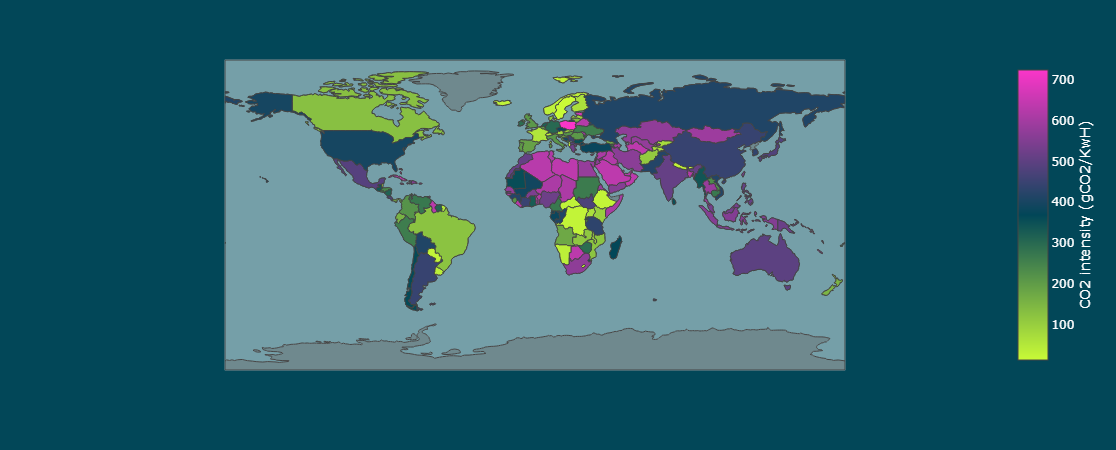
\includegraphics[width=0.9\textwidth]{imagenes/CC_5.png}
\end{center}

\end{document}
